\documentclass[12pt]{article}

\usepackage[letterpaper,margin=1in]{geometry}
\usepackage[T1]{fontenc}
\usepackage{lmodern}
\usepackage{microtype}
\usepackage{amsmath,amssymb}
\usepackage{booktabs}
\usepackage{graphicx}
\usepackage{natbib}
\usepackage{setspace}
\usepackage{xcolor}
\usepackage{tikz}
\usepackage[hidelinks]{hyperref}

\hypersetup{
  pdftitle={Bounded Evolution in a Reflexive Digital Population: A Local SAEE Characterization},
  pdfauthor={Bin Zhang; Xiaojuan Sun},
  pdfsubject={Letter submitted to Artificial Life},
  pdfkeywords={artificial life, digital evolution, lineage, bounded dynamics, reflexive systems}
}

\setlength{\parindent}{1.5em}
\setlength{\parskip}{0pt}

\title{Bounded Evolution in a Reflexive Digital Population:\\
A Local SAEE Characterization}
\author{Bin Zhang$^{1,*}$ \quad Xiaojuan Sun$^{2}$\\[0.5em]
\small $^1$Shanxi Youqibing E-Commerce Co., Ltd., Yuncheng, Shanxi, China\\
\small $^2$Department of Physical Education, Yuncheng University,
Yuncheng, Shanxi 044000, China\\
\small $^*$Corresponding author: \texttt{joy7759@gmail.com}\\
\small ORCID: Bin Zhang 0009-0002-8861-1481; Xiaojuan Sun 0009-0003-4705-1809}
\date{}

\begin{document}
\maketitle

\begin{abstract}
Open-ended evolution is often discussed through continued novelty, diversity,
or major transitions. Equally important is identifying when a digital
evolution system is bounded. We report an artifact-backed local
characterization of SAEE, a digital population system whose formal state
includes population, transformation, selection, lineage, observer, and
identity terms. Two existing evidence surfaces are kept separate. In a
100-generation fixed-kernel run, population size remains eight, mean fitness
increases from 0.5993 to 0.6360, the final-to-initial ten-generation fitness
variance ratio is 0.383, and no collapse event is recorded. The associated
lineage record contains 808 nodes and 1,590 parent--child edges with valid
endpoints. In a separate six-generation reflexive-analysis record, one
categorical state signature recurs at all observations, semantic drift remains
0.2 under a configured bound of 0.32, and all points receive the local
\texttt{stable\_regime} label. These measurements support a bounded,
convergent interpretation for the recorded artifacts, not mathematical
attractor existence or open-ended evolution. The result demonstrates a
claim-scoped method for reporting negative evidence about open-endedness while
preserving provenance and measurement boundaries.
\end{abstract}

\noindent\textbf{Keywords:} artificial life; digital evolution; lineage;
bounded dynamics; reflexive systems; empirical characterization

\newpage
\setstretch{1.85}

\section{Introduction}

Artificial life studies constructed systems that realize or simulate
life-like processes in software, hardware, and wetware \citep{dorin2024}.
Open-ended evolution remains a central challenge, but long execution alone is
not evidence of continuing evolutionary innovation \citep{taylor2016,hintze2019}.
Measurement proposals therefore examine novelty, diversity, complexity, and
ecological or phylogenetic structure \citep{dolson2019,moreno2025}.

This Letter asks a narrower question: what can be stated when a digital
population remains viable but its recorded behavior is strongly bounded? We
analyze existing SAEE artifacts without rerunning the system or changing its
kernel. The contribution is not a new open-ended mechanism. It is a
provenance-bounded characterization that distinguishes observed convergence,
recurring discrete state, and lineage endpoint integrity from stronger claims
such as formal attractor existence, cross-seed robustness, or universal law.

\section{System and measurements}

The paper-facing formal state is
\(
  (\Omega,G,T,S,L,R,\mu)
\), with population update
\begin{equation}
  P_{t+1}=S_{\theta_t}\!\left(T_{\phi_t}(P_t)\right).
\end{equation}
Here \(L\) records lineage and \(R\) represents observer state. This notation
describes the system boundary; the 100-generation runtime analyzed below uses
a fixed deterministic kernel and does not empirically establish operator
co-evolution.

We preserve two distinct evidence surfaces. The first is a 100-generation
v1.0 run configured with population size eight and deterministic identifier and
weight updates. A collapse is logged if population size falls below two or the
survivor count becomes zero. The reported convergence label compares mean
fitness variance over the first and final ten generations; the run is labeled
converging when the latter is less than 75\% of the former. Population turnover
is Jaccard distance between consecutive genome-identifier sets.

The second surface is a six-generation Phase II analysis of a different v0.8
record. Its semantic-drift measure is one minus the fraction of identity-anchor
terms retained among dominant feedback terms. A categorical signature combines
identity stability, drift boundedness, population density, and mutation
activity. A signature observed at least twice is called an empirical attractor
candidate by the local implementation. This is recurrence under a discrete
rule, not a continuous-state attractor test.

\section{Observed dynamics}

Figure~\ref{fig:long-horizon} summarizes the long-horizon trace. Mean fitness
rises from 0.599284 to 0.636003. Mean variance over generations 91--100 is
0.383 times the mean over generations 1--10, satisfying the implemented
convergence rule. Population remains eight throughout, no collapse is logged,
and mean genome-set turnover is 0.545531. Turnover therefore continues even
while fitness variance contracts.

\begin{figure}[t]
  \centering
  \resizebox{\textwidth}{!}{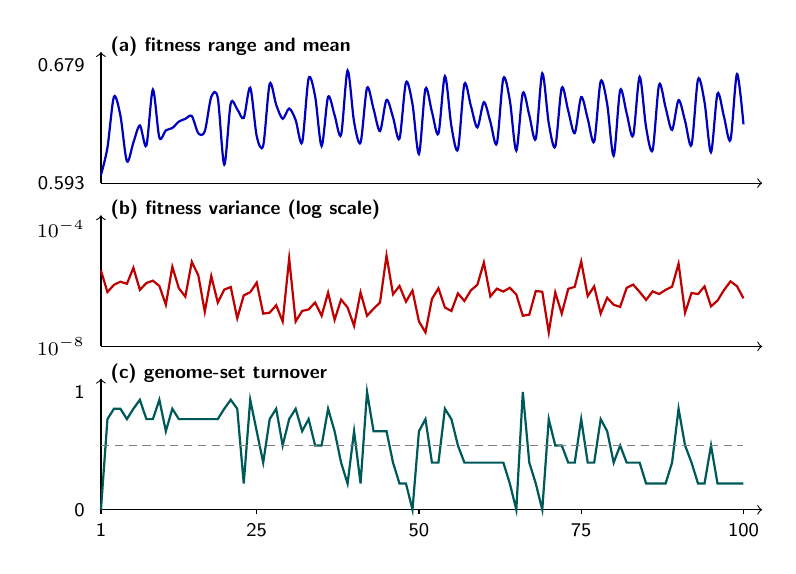
\begin{tikzpicture}[x=0.68cm,y=0.68cm,font=\sffamily\scriptsize]
% Panel A
\begin{scope}[shift={(0,6.1)}]
\draw[->] (0,0) -- (12.35,0);
\draw[->] (0,0) -- (0,2.45);
\fill[blue!12] (0.0000,0.2448) (0.1212,0.7045) (0.2424,1.6724) (0.3636,1.3293) (0.4848,0.4650) (0.6061,0.8637) (0.7273,1.1290) (0.8485,0.7570) (0.9697,1.8093) (1.0909,0.8932) (1.2121,1.0022) (1.3333,1.1373) (1.4545,1.1966) (1.5758,1.2299) (1.6970,1.3833) (1.8182,1.0064) (1.9394,0.9881) (2.0606,1.6754) (2.1818,1.6133) (2.3030,0.3934) (2.4242,1.5508) (2.5455,1.3950) (2.6667,1.2589) (2.7879,1.8183) (2.9091,0.9305) (3.0303,0.7107) (3.1515,1.8732) (3.2727,1.4899) (3.3939,1.2152) (3.5152,1.4814) (3.6364,1.1947) (3.7576,0.7771) (3.8788,1.9755) (4.0000,1.6379) (4.1212,0.7073) (4.2424,1.6491) (4.3636,1.2798) (4.4848,0.9266) (4.6061,2.1185) (4.7273,1.1519) (4.8485,0.7812) (4.9697,1.7895) (5.0909,1.4002) (5.2121,0.9918) (5.3333,1.6483) (5.4545,1.2557) (5.5758,0.8665) (5.6970,1.8909) (5.8182,1.5017) (5.9394,0.5573) (6.0606,1.7694) (6.1818,1.3571) (6.3030,0.9679) (6.4242,2.0196) (6.5455,1.0778) (6.6667,0.6587) (6.7879,1.8670) (6.9091,1.4778) (7.0303,1.0886) (7.1515,1.5673) (7.2727,1.1686) (7.3939,0.7794) (7.5152,1.9876) (7.6364,1.5792) (7.7576,0.6348) (7.8788,1.6925) (8.0000,1.2852) (8.1212,0.8592) (8.2424,2.0754) (8.3636,1.1286) (8.4848,0.7177) (8.6061,1.7957) (8.7273,1.3845) (8.8485,0.9772) (8.9697,1.6624) (9.0909,1.2242) (9.2121,0.8169) (9.3333,1.9199) (9.4545,1.5025) (9.5758,0.5332) (9.6970,1.7495) (9.8182,1.3422) (9.9394,0.9349) (10.0606,2.0090) (10.1818,1.0585) (10.3030,0.6513) (10.4242,1.8675) (10.5455,1.4415) (10.6667,1.0342) (10.7879,1.6002) (10.9091,1.1766) (11.0303,0.7505) (11.1515,1.9668) (11.2727,1.5595) (11.3939,0.6090) (11.5152,1.6859) (11.6364,1.2758) (11.7576,0.8686) (11.8788,2.0848) (12.0000,1.1155) (12.0000,1.0752) (11.8788,1.9812) (11.7576,0.7521) (11.6364,1.2019) (11.5152,1.6510) (11.3939,0.5588) (11.2727,1.4539) (11.1515,1.9020) (11.0303,0.6711) (10.9091,1.1498) (10.7879,1.4312) (10.6667,0.9610) (10.5455,1.3827) (10.4242,1.8128) (10.3030,0.5885) (10.1818,1.0092) (10.0606,1.9537) (9.9394,0.8490) (9.8182,1.2564) (9.6970,1.7038) (9.5758,0.4828) (9.4545,1.4533) (9.3333,1.8886) (9.2121,0.7192) (9.0909,1.1705) (8.9697,1.4690) (8.8485,0.9017) (8.7273,1.2960) (8.6061,1.7611) (8.4848,0.6503) (8.3636,1.1107) (8.2424,2.0187) (8.1212,0.7948) (8.0000,1.2575) (7.8788,1.6709) (7.7576,0.5811) (7.6364,1.5138) (7.5152,1.9235) (7.3939,0.7085) (7.2727,1.1183) (7.1515,1.3833) (7.0303,1.0062) (6.9091,1.4080) (6.7879,1.8173) (6.6667,0.5775) (6.5455,1.0442) (6.4242,1.9795) (6.3030,0.8927) (6.1818,1.2996) (6.0606,1.7533) (5.9394,0.5363) (5.8182,1.4400) (5.6970,1.8492) (5.5758,0.7888) (5.4545,1.1940) (5.3333,1.4458) (5.2121,0.9512) (5.0909,1.3690) (4.9697,1.7660) (4.8485,0.7221) (4.7273,1.1313) (4.6061,2.0852) (4.4848,0.8804) (4.3636,1.2552) (4.2424,1.5823) (4.1212,0.6809) (4.0000,1.5891) (3.8788,1.9375) (3.7576,0.7430) (3.6364,1.1675) (3.5152,1.2762) (3.3939,1.1883) (3.2727,1.4432) (3.1515,1.8407) (3.0303,0.6822) (2.9091,0.8397) (2.7879,1.7399) (2.6667,1.1807) (2.5455,1.3671) (2.4242,1.4522) (2.3030,0.3066) (2.1818,1.5732) (2.0606,1.5424) (1.9394,0.9552) (1.8182,0.8609) (1.6970,1.1448) (1.5758,1.1756) (1.4545,1.1142) (1.3333,0.9144) (1.2121,0.9679) (1.0909,0.8038) (0.9697,1.6912) (0.8485,0.6535) (0.7273,1.0449) (0.6061,0.6595) (0.4848,0.3564) (0.3636,1.2168) (0.2424,1.5719) (0.1212,0.6198) (0.0000,0.0815) -- cycle;
\draw[blue!75!black,thick] plot[smooth] coordinates {(0.0000,0.1524) (0.1212,0.6614) (0.2424,1.6118) (0.3636,1.2593) (0.4848,0.4081) (0.6061,0.7587) (0.7273,1.0771) (0.8485,0.7010) (0.9697,1.7470) (1.0909,0.8504) (1.2121,0.9857) (1.3333,1.0292) (1.4545,1.1483) (1.5758,1.1997) (1.6970,1.2524) (1.8182,0.9318) (1.9394,0.9680) (2.0606,1.6123) (2.1818,1.5940) (2.3030,0.3452) (2.4242,1.4870) (2.5455,1.3783) (2.6667,1.2178) (2.7879,1.7832) (2.9091,0.8785) (3.0303,0.7010) (3.1515,1.8535) (3.2727,1.4639) (3.3939,1.2013) (3.5152,1.3939) (3.6364,1.1779) (3.7576,0.7592) (3.8788,1.9552) (4.0000,1.6196) (4.1212,0.6942) (4.2424,1.6102) (4.3636,1.2702) (4.4848,0.9013) (4.6061,2.1021) (4.7273,1.1458) (4.8485,0.7572) (4.9697,1.7772) (5.0909,1.3851) (5.2121,0.9727) (5.3333,1.5541) (5.4545,1.2317) (5.5758,0.8306) (5.6970,1.8788) (5.8182,1.4762) (5.9394,0.5447) (6.0606,1.7615) (6.1818,1.3302) (6.3030,0.9243) (6.4242,1.9987) (6.5455,1.0607) (6.6667,0.6298) (6.7879,1.8491) (6.9091,1.4417) (7.0303,1.0399) (7.1515,1.5123) (7.2727,1.1451) (7.3939,0.7408) (7.5152,1.9550) (7.6364,1.5470) (7.7576,0.6071) (7.8788,1.6820) (8.0000,1.2681) (8.1212,0.8277) (8.2424,2.0493) (8.3636,1.1174) (8.4848,0.6815) (8.6061,1.7796) (8.7273,1.3492) (8.8485,0.9330) (8.9697,1.6073) (9.0909,1.2026) (9.2121,0.7762) (9.3333,1.9015) (9.4545,1.4771) (9.5758,0.5112) (9.6970,1.7359) (9.8182,1.3045) (9.9394,0.8850) (10.0606,1.9845) (10.1818,1.0383) (10.3030,0.6160) (10.4242,1.8374) (10.5455,1.4118) (10.6667,0.9932) (10.7879,1.5509) (10.9091,1.1609) (11.0303,0.7137) (11.1515,1.9395) (11.2727,1.5119) (11.3939,0.5774) (11.5152,1.6717) (11.6364,1.2383) (11.7576,0.8097) (11.8788,2.0375) (12.0000,1.0971)};
\node[anchor=west,font=\sffamily\bfseries\scriptsize] at (0,2.55) {(a) fitness range and mean};
\node[anchor=east] at (-0.12,0) {0.593};
\node[anchor=east] at (-0.12,2.2) {0.679};
\end{scope}
% Panel B
\begin{scope}[shift={(0,3.05)}]
\draw[->] (0,0) -- (12.35,0);
\draw[->] (0,0) -- (0,2.45);
\draw[red!75!black,thick] plot coordinates {(0.0000,1.4183) (0.1212,1.0148) (0.2424,1.1494) (0.3636,1.2093) (0.4848,1.1699) (0.6061,1.4676) (0.7273,1.0555) (0.8485,1.1838) (0.9697,1.2281) (1.0909,1.1292) (1.2121,0.7782) (1.3333,1.4873) (1.4545,1.0877) (1.5758,0.9296) (1.6970,1.5800) (1.8182,1.3273) (1.9394,0.6469) (2.0606,1.3131) (2.1818,0.8202) (2.3030,1.0612) (2.4242,1.1094) (2.5455,0.5248) (2.6667,0.9528) (2.7879,1.0114) (2.9091,1.1920) (3.0303,0.6127) (3.1515,0.6304) (3.2727,0.7689) (3.3939,0.4648) (3.5152,1.6402) (3.6364,0.4648) (3.7576,0.6623) (3.8788,0.6904) (4.0000,0.8202) (4.1212,0.5728) (4.2424,1.0043) (4.3636,0.4967) (4.4848,0.8751) (4.6061,0.7272) (4.7273,0.3844) (4.8485,1.0079) (4.9697,0.5728) (5.0909,0.7033) (5.2121,0.8202) (5.3333,1.6965) (5.4545,0.9740) (5.5758,1.1292) (5.6970,0.8352) (5.8182,1.0437) (5.9394,0.4648) (6.0606,0.2624) (6.1818,0.8870) (6.3030,1.0852) (6.4242,0.7272) (6.5455,0.6623) (6.6667,0.9896) (6.7879,0.8492) (6.9091,1.0467) (7.0303,1.1514) (7.1515,1.5665) (7.2727,0.9344) (7.3939,1.0775) (7.5152,1.0248) (7.6364,1.0952) (7.7576,0.9699) (7.8788,0.5728) (8.0000,0.5935) (8.1212,1.0344) (8.2424,1.0215) (8.3636,0.2624) (8.4848,1.0079) (8.6061,0.6127) (8.7273,1.0748) (8.8485,1.1139) (8.9697,1.5851) (9.0909,0.9392) (9.2121,1.1206) (9.3333,0.6127) (9.4545,0.9093) (9.5758,0.7782) (9.6970,0.7383) (9.8182,1.0927) (9.9394,1.1552) (10.0606,1.0182) (10.1818,0.8689) (10.3030,1.0281) (10.4242,0.9780) (10.5455,1.0555) (10.6667,1.1162) (10.7879,1.5441) (10.9091,0.6304) (11.0303,0.9971) (11.1515,0.9780) (11.2727,1.1206) (11.3939,0.7490) (11.5152,0.8560) (11.6364,1.0526) (11.7576,1.2152) (11.8788,1.1249) (12.0000,0.8984)};
\node[anchor=west,font=\sffamily\bfseries\scriptsize] at (0,2.55) {(b) fitness variance (log scale)};
\node[anchor=east] at (-0.12,0) {$10^{-8}$};
\node[anchor=east] at (-0.12,2.2) {$10^{-4}$};
\end{scope}
% Panel C
\begin{scope}[shift={(0,0)}]
\draw[->] (0,0) -- (12.35,0);
\draw[->] (0,0) -- (0,2.45);
\draw[teal!70!black,thick] plot coordinates {(0.0000,0.0000) (0.1212,1.6923) (0.2424,1.8857) (0.3636,1.8857) (0.4848,1.6923) (0.6061,1.8857) (0.7273,2.0533) (0.8485,1.6923) (0.9697,1.6923) (1.0909,2.0533) (1.2121,1.4667) (1.3333,1.8857) (1.4545,1.6923) (1.5758,1.6923) (1.6970,1.6923) (1.8182,1.6923) (1.9394,1.6923) (2.0606,1.6923) (2.1818,1.6923) (2.3030,1.8857) (2.4242,2.0533) (2.5455,1.8857) (2.6667,0.4889) (2.7879,2.0533) (2.9091,1.4667) (3.0303,0.8800) (3.1515,1.6923) (3.2727,1.8857) (3.3939,1.2000) (3.5152,1.6923) (3.6364,1.8857) (3.7576,1.4667) (3.8788,1.6923) (4.0000,1.2000) (4.1212,1.2000) (4.2424,1.8857) (4.3636,1.4667) (4.4848,0.8800) (4.6061,0.4889) (4.7273,1.4667) (4.8485,0.4889) (4.9697,2.2000) (5.0909,1.4667) (5.2121,1.4667) (5.3333,1.4667) (5.4545,0.8800) (5.5758,0.4889) (5.6970,0.4889) (5.8182,0.0000) (5.9394,1.4667) (6.0606,1.6923) (6.1818,0.8800) (6.3030,0.8800) (6.4242,1.8857) (6.5455,1.6923) (6.6667,1.2000) (6.7879,0.8800) (6.9091,0.8800) (7.0303,0.8800) (7.1515,0.8800) (7.2727,0.8800) (7.3939,0.8800) (7.5152,0.8800) (7.6364,0.4889) (7.7576,0.0000) (7.8788,2.2000) (8.0000,0.8800) (8.1212,0.4889) (8.2424,0.0000) (8.3636,1.6923) (8.4848,1.2000) (8.6061,1.2000) (8.7273,0.8800) (8.8485,0.8800) (8.9697,1.6923) (9.0909,0.8800) (9.2121,0.8800) (9.3333,1.6923) (9.4545,1.4667) (9.5758,0.8800) (9.6970,1.2000) (9.8182,0.8800) (9.9394,0.8800) (10.0606,0.8800) (10.1818,0.4889) (10.3030,0.4889) (10.4242,0.4889) (10.5455,0.4889) (10.6667,0.8800) (10.7879,1.8857) (10.9091,1.2000) (11.0303,0.8800) (11.1515,0.4889) (11.2727,0.4889) (11.3939,1.2000) (11.5152,0.4889) (11.6364,0.4889) (11.7576,0.4889) (11.8788,0.4889) (12.0000,0.4889)};
\draw[densely dashed,gray] (0,1.2) -- (12,1.2);
\node[anchor=west,font=\sffamily\bfseries\scriptsize] at (0,2.55) {(c) genome-set turnover};
\node[anchor=east] at (-0.12,0) {0};
\node[anchor=east] at (-0.12,2.2) {1};
\foreach \g in {1,25,50,75,100} {\pgfmathsetmacro{\gx}{(\g-1)/99*12} \draw (\gx,0) -- (\gx,-0.08) node[below]{\g};}
\end{scope}
\end{tikzpicture}
}
  \caption{Existing 100-generation v1.0 trace. The shaded band is the observed
  fitness range; variance uses a logarithmic axis. Turnover is Jaccard distance
  between consecutive population identifier sets.}
  \label{fig:long-horizon}
\end{figure}

The lineage record contains 808 nodes and 1,590 directed parent--child edges.
Every recorded edge endpoint resolves to a node identifier, yielding a
branching-density summary of 1.967822 edges per node. The implementation does
not independently perform cycle detection, so this result is endpoint
integrity under a declared lineage-DAG type, not a graph-theoretic proof.

In the separate Phase II record, population is six at each observation,
semantic drift is 0.2 against a 0.32 bound, and one categorical signature
recurs six times. All points are labeled \texttt{stable\_regime}; no
cross-regime transition is recorded. Figure~\ref{fig:lineage-phase2} displays
the lineage surface and the constant drift series. The repository's later
\texttt{stable\_lineage\_basin} label compresses these observations but is not
a measured basin volume or calibrated probability.

\begin{figure}[t]
  \centering
  \resizebox{\textwidth}{!}{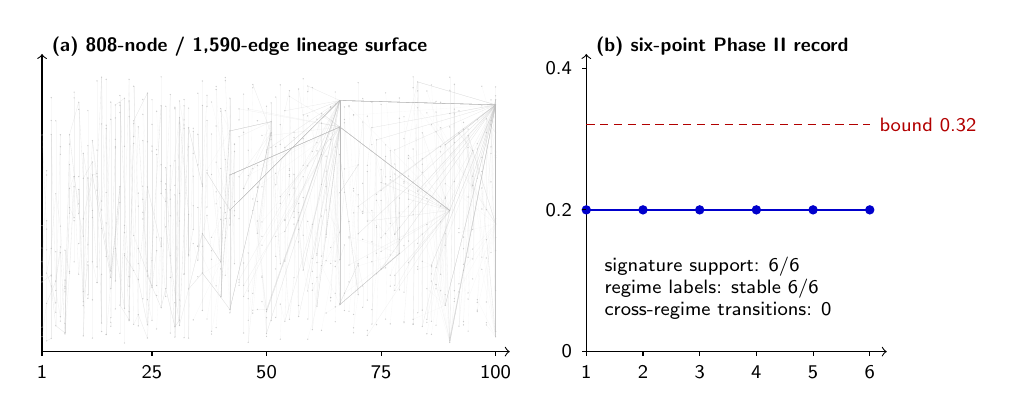
\begin{tikzpicture}[x=0.72cm,y=0.72cm,font=\sffamily\scriptsize]
\begin{scope}
\draw[->] (0,0) -- (8.25,0);
\draw[->] (0,0) -- (0,5.25);
\node[anchor=west,font=\sffamily\bfseries\scriptsize] at (0,5.38) {(a) 808-node / 1,590-edge lineage surface};
\draw[gray!55,opacity=0.10,line width=0.12pt] (0.0000,1.2291) -- (0.1616,1.3493);
\draw[gray!55,opacity=0.10,line width=0.12pt] (0.0000,1.5838) -- (0.0000,2.2231);
\draw[gray!55,opacity=0.10,line width=0.12pt] (0.0808,0.1886) -- (0.1616,0.2319);
\draw[gray!55,opacity=0.10,line width=0.12pt] (0.0000,1.3219) -- (0.0808,3.1151);
\draw[gray!55,opacity=0.10,line width=0.12pt] (0.0000,3.8208) -- (0.0808,2.1601);
\draw[gray!55,opacity=0.10,line width=0.12pt] (0.0000,1.8273) -- (0.0000,0.4307);
\draw[gray!55,opacity=0.10,line width=0.12pt] (0.0808,1.3845) -- (0.1616,1.1571);
\draw[gray!55,opacity=0.10,line width=0.12pt] (0.0000,0.2623) -- (0.0808,0.8506);
\draw[gray!55,opacity=0.10,line width=0.12pt] (0.0000,1.2291) -- (0.1616,1.3493);
\draw[gray!55,opacity=0.10,line width=0.12pt] (0.1616,1.3493) -- (0.1616,1.3341);
\draw[gray!55,opacity=0.10,line width=0.12pt] (0.0808,0.1886) -- (0.1616,0.2319);
\draw[gray!55,opacity=0.10,line width=0.12pt] (0.0808,0.1886) -- (0.0808,2.3086);
\draw[gray!55,opacity=0.10,line width=0.12pt] (0.1616,0.2319) -- (0.1616,3.8299);
\draw[gray!55,opacity=0.10,line width=0.12pt] (0.0000,1.3219) -- (0.0808,3.1151);
\draw[gray!55,opacity=0.10,line width=0.12pt] (0.0808,3.1151) -- (0.0808,3.1894);
\draw[gray!55,opacity=0.10,line width=0.12pt] (0.0000,3.8208) -- (0.0808,2.1601);
\draw[gray!55,opacity=0.10,line width=0.12pt] (0.0808,2.1601) -- (0.0808,1.7951);
\draw[gray!55,opacity=0.10,line width=0.12pt] (0.0808,1.3845) -- (0.1616,1.1571);
\draw[gray!55,opacity=0.10,line width=0.12pt] (0.0808,1.3845) -- (0.1616,1.8208);
\draw[gray!55,opacity=0.10,line width=0.12pt] (0.1616,1.1571) -- (0.2424,0.4559);
\draw[gray!55,opacity=0.10,line width=0.12pt] (0.0000,0.2623) -- (0.0808,0.8506);
\draw[gray!55,opacity=0.10,line width=0.12pt] (0.0808,0.8506) -- (0.2424,1.2426);
\draw[gray!55,opacity=0.10,line width=0.12pt] (0.0000,1.2291) -- (0.1616,1.3493);
\draw[gray!55,opacity=0.10,line width=0.12pt] (0.1616,1.3493) -- (0.1616,1.3341);
\draw[gray!55,opacity=0.10,line width=0.12pt] (0.1616,1.3493) -- (0.1616,4.4798);
\draw[gray!55,opacity=0.10,line width=0.12pt] (0.1616,1.3341) -- (0.2424,0.6935);
\draw[gray!55,opacity=0.10,line width=0.12pt] (0.0808,0.1886) -- (0.1616,0.2319);
\draw[gray!55,opacity=0.10,line width=0.12pt] (0.1616,0.2319) -- (0.1616,3.8299);
\draw[gray!55,opacity=0.10,line width=0.12pt] (0.1616,0.2319) -- (0.1616,4.0769);
\draw[gray!55,opacity=0.10,line width=0.12pt] (0.1616,3.8299) -- (0.2424,1.0784);
\draw[gray!55,opacity=0.10,line width=0.12pt] (0.0808,1.3845) -- (0.1616,1.1571);
\draw[gray!55,opacity=0.10,line width=0.12pt] (0.0808,1.3845) -- (0.1616,1.8208);
\draw[gray!55,opacity=0.10,line width=0.12pt] (0.1616,1.1571) -- (0.2424,0.4559);
\draw[gray!55,opacity=0.10,line width=0.12pt] (0.1616,1.1571) -- (0.2424,0.8593);
\draw[gray!55,opacity=0.10,line width=0.12pt] (0.2424,0.4559) -- (0.4040,0.3304);
\draw[gray!55,opacity=0.10,line width=0.12pt] (0.1616,1.8208) -- (0.2424,2.7842);
\draw[gray!55,opacity=0.10,line width=0.12pt] (0.0808,0.8506) -- (0.2424,1.2426);
\draw[gray!55,opacity=0.10,line width=0.12pt] (0.2424,1.2426) -- (0.3232,1.8472);
\draw[gray!55,opacity=0.10,line width=0.12pt] (0.1616,1.3341) -- (0.2424,0.6935);
\draw[gray!55,opacity=0.10,line width=0.12pt] (0.2424,0.6935) -- (0.3232,3.8246);
\draw[gray!55,opacity=0.10,line width=0.12pt] (0.1616,3.8299) -- (0.2424,1.0784);
\draw[gray!55,opacity=0.10,line width=0.12pt] (0.2424,1.0784) -- (0.3232,0.6152);
\draw[gray!55,opacity=0.10,line width=0.12pt] (0.1616,1.1571) -- (0.2424,0.4559);
\draw[gray!55,opacity=0.10,line width=0.12pt] (0.1616,1.1571) -- (0.2424,0.8593);
\draw[gray!55,opacity=0.10,line width=0.12pt] (0.2424,0.4559) -- (0.4040,0.3304);
\draw[gray!55,opacity=0.10,line width=0.12pt] (0.2424,0.4559) -- (0.2424,4.0706);
\draw[gray!55,opacity=0.10,line width=0.12pt] (0.4040,0.3304) -- (0.4040,0.4950);
\draw[gray!55,opacity=0.10,line width=0.12pt] (0.2424,0.8593) -- (0.2424,1.7616);
\draw[gray!55,opacity=0.10,line width=0.12pt] (0.1616,1.8208) -- (0.2424,2.7842);
\draw[gray!55,opacity=0.10,line width=0.12pt] (0.2424,2.7842) -- (0.3232,2.2128);
\draw[gray!55,opacity=0.10,line width=0.12pt] (0.0808,0.8506) -- (0.2424,1.2426);
\draw[gray!55,opacity=0.10,line width=0.12pt] (0.2424,1.2426) -- (0.3232,1.8472);
\draw[gray!55,opacity=0.10,line width=0.12pt] (0.2424,1.2426) -- (0.3232,1.7444);
\draw[gray!55,opacity=0.10,line width=0.12pt] (0.3232,1.8472) -- (0.4040,0.3120);
\draw[gray!55,opacity=0.10,line width=0.12pt] (0.2424,0.6935) -- (0.3232,3.8246);
\draw[gray!55,opacity=0.10,line width=0.12pt] (0.3232,3.8246) -- (0.3232,3.4791);
\draw[gray!55,opacity=0.10,line width=0.12pt] (0.2424,1.0784) -- (0.3232,0.6152);
\draw[gray!55,opacity=0.10,line width=0.12pt] (0.3232,0.6152) -- (0.4040,1.2608);
\draw[gray!55,opacity=0.10,line width=0.12pt] (0.2424,0.4559) -- (0.4040,0.3304);
\draw[gray!55,opacity=0.10,line width=0.12pt] (0.4040,0.3304) -- (0.4040,0.4950);
\draw[gray!55,opacity=0.10,line width=0.12pt] (0.4040,0.3304) -- (0.4040,1.7881);
\draw[gray!55,opacity=0.10,line width=0.12pt] (0.4040,0.4950) -- (0.4848,2.4403);
\draw[gray!55,opacity=0.10,line width=0.12pt] (0.2424,2.7842) -- (0.3232,2.2128);
\draw[gray!55,opacity=0.10,line width=0.12pt] (0.3232,2.2128) -- (0.4040,1.0547);
\draw[gray!55,opacity=0.10,line width=0.12pt] (0.2424,1.2426) -- (0.3232,1.8472);
\draw[gray!55,opacity=0.10,line width=0.12pt] (0.2424,1.2426) -- (0.3232,1.7444);
\draw[gray!55,opacity=0.10,line width=0.12pt] (0.3232,1.8472) -- (0.4040,0.3120);
\draw[gray!55,opacity=0.10,line width=0.12pt] (0.3232,1.8472) -- (0.3232,3.6136);
\draw[gray!55,opacity=0.10,line width=0.12pt] (0.4040,0.3120) -- (0.4848,3.8259);
\draw[gray!55,opacity=0.10,line width=0.12pt] (0.3232,1.7444) -- (0.3232,0.5378);
\draw[gray!55,opacity=0.10,line width=0.12pt] (0.3232,0.6152) -- (0.4040,1.2608);
\draw[gray!55,opacity=0.10,line width=0.12pt] (0.4040,1.2608) -- (0.4040,1.1163);
\draw[gray!55,opacity=0.10,line width=0.12pt] (0.2424,0.4559) -- (0.4040,0.3304);
\draw[gray!55,opacity=0.10,line width=0.12pt] (0.4040,0.3304) -- (0.4040,0.4950);
\draw[gray!55,opacity=0.10,line width=0.12pt] (0.4040,0.3304) -- (0.4040,1.7881);
\draw[gray!55,opacity=0.10,line width=0.12pt] (0.4040,0.3304) -- (0.4040,1.1511);
\draw[gray!55,opacity=0.10,line width=0.12pt] (0.4040,0.4950) -- (0.4848,2.4403);
\draw[gray!55,opacity=0.10,line width=0.12pt] (0.4040,0.4950) -- (0.4848,2.5410);
\draw[gray!55,opacity=0.10,line width=0.12pt] (0.4848,2.4403) -- (0.4848,2.8785);
\draw[gray!55,opacity=0.10,line width=0.12pt] (0.4040,1.7881) -- (0.4848,1.4109);
\draw[gray!55,opacity=0.10,line width=0.12pt] (0.3232,2.2128) -- (0.4040,1.0547);
\draw[gray!55,opacity=0.10,line width=0.12pt] (0.4040,1.0547) -- (0.4848,3.3002);
\draw[gray!55,opacity=0.10,line width=0.12pt] (0.3232,1.8472) -- (0.4040,0.3120);
\draw[gray!55,opacity=0.10,line width=0.12pt] (0.4040,0.3120) -- (0.4848,3.8259);
\draw[gray!55,opacity=0.10,line width=0.12pt] (0.4040,0.3120) -- (0.4848,1.3839);
\draw[gray!55,opacity=0.10,line width=0.12pt] (0.4848,3.8259) -- (0.6465,2.4359);
\draw[gray!55,opacity=0.10,line width=0.12pt] (0.4040,0.4950) -- (0.4848,2.4403);
\draw[gray!55,opacity=0.10,line width=0.12pt] (0.4040,0.4950) -- (0.4848,2.5410);
\draw[gray!55,opacity=0.10,line width=0.12pt] (0.4848,2.4403) -- (0.4848,2.8785);
\draw[gray!55,opacity=0.10,line width=0.12pt] (0.4848,2.4403) -- (0.4848,3.6592);
\draw[gray!55,opacity=0.10,line width=0.12pt] (0.4848,2.8785) -- (0.5657,3.0853);
\draw[gray!55,opacity=0.10,line width=0.12pt] (0.4848,2.5410) -- (0.5657,2.3617);
\draw[gray!55,opacity=0.10,line width=0.12pt] (0.4040,1.7881) -- (0.4848,1.4109);
\draw[gray!55,opacity=0.10,line width=0.12pt] (0.4848,1.4109) -- (0.5657,3.0838);
\draw[gray!55,opacity=0.10,line width=0.12pt] (0.4040,1.0547) -- (0.4848,3.3002);
\draw[gray!55,opacity=0.10,line width=0.12pt] (0.4848,3.3002) -- (0.5657,2.3085);
\draw[gray!55,opacity=0.10,line width=0.12pt] (0.4040,0.3120) -- (0.4848,3.8259);
\draw[gray!55,opacity=0.10,line width=0.12pt] (0.4040,0.3120) -- (0.4848,1.3839);
\draw[gray!55,opacity=0.10,line width=0.12pt] (0.4848,3.8259) -- (0.6465,2.4359);
\draw[gray!55,opacity=0.10,line width=0.12pt] (0.4848,3.8259) -- (0.6465,4.3981);
\draw[gray!55,opacity=0.10,line width=0.12pt] (0.6465,2.4359) -- (0.6465,2.8599);
\draw[gray!55,opacity=0.10,line width=0.12pt] (0.4848,1.3839) -- (0.5657,2.9105);
\draw[gray!55,opacity=0.10,line width=0.12pt] (0.4848,2.8785) -- (0.5657,3.0853);
\draw[gray!55,opacity=0.10,line width=0.12pt] (0.5657,3.0853) -- (0.6465,2.6044);
\draw[gray!55,opacity=0.10,line width=0.12pt] (0.4848,2.5410) -- (0.5657,2.3617);
\draw[gray!55,opacity=0.10,line width=0.12pt] (0.5657,2.3617) -- (0.5657,4.5763);
\draw[gray!55,opacity=0.10,line width=0.12pt] (0.4848,1.4109) -- (0.5657,3.0838);
\draw[gray!55,opacity=0.10,line width=0.12pt] (0.5657,3.0838) -- (0.5657,4.4753);
\draw[gray!55,opacity=0.10,line width=0.12pt] (0.4848,3.3002) -- (0.5657,2.3085);
\draw[gray!55,opacity=0.10,line width=0.12pt] (0.5657,2.3085) -- (0.5657,1.5832);
\draw[gray!55,opacity=0.10,line width=0.12pt] (0.4848,3.8259) -- (0.6465,2.4359);
\draw[gray!55,opacity=0.10,line width=0.12pt] (0.4848,3.8259) -- (0.6465,4.3981);
\draw[gray!55,opacity=0.10,line width=0.12pt] (0.6465,2.4359) -- (0.6465,2.8599);
\draw[gray!55,opacity=0.10,line width=0.12pt] (0.6465,2.4359) -- (0.7273,2.0354);
\draw[gray!55,opacity=0.10,line width=0.12pt] (0.6465,2.8599) -- (0.7273,0.8790);
\draw[gray!55,opacity=0.10,line width=0.12pt] (0.6465,4.3981) -- (0.7273,3.0572);
\draw[gray!55,opacity=0.10,line width=0.12pt] (0.4848,1.3839) -- (0.5657,2.9105);
\draw[gray!55,opacity=0.10,line width=0.12pt] (0.5657,2.9105) -- (0.6465,1.3655);
\draw[gray!55,opacity=0.10,line width=0.12pt] (0.5657,3.0853) -- (0.6465,2.6044);
\draw[gray!55,opacity=0.10,line width=0.12pt] (0.6465,2.6044) -- (0.6465,4.2715);
\draw[gray!55,opacity=0.10,line width=0.12pt] (0.4848,3.8259) -- (0.6465,2.4359);
\draw[gray!55,opacity=0.10,line width=0.12pt] (0.4848,3.8259) -- (0.6465,4.3981);
\draw[gray!55,opacity=0.10,line width=0.12pt] (0.6465,2.4359) -- (0.6465,2.8599);
\draw[gray!55,opacity=0.10,line width=0.12pt] (0.6465,2.4359) -- (0.7273,2.0354);
\draw[gray!55,opacity=0.10,line width=0.12pt] (0.6465,2.4359) -- (0.6465,1.9055);
\draw[gray!55,opacity=0.10,line width=0.12pt] (0.6465,2.8599) -- (0.7273,0.8790);
\draw[gray!55,opacity=0.10,line width=0.12pt] (0.6465,2.8599) -- (0.7273,0.8102);
\draw[gray!55,opacity=0.10,line width=0.12pt] (0.7273,0.8790) -- (0.8081,1.5276);
\draw[gray!55,opacity=0.10,line width=0.12pt] (0.7273,2.0354) -- (0.7273,3.4958);
\draw[gray!55,opacity=0.10,line width=0.12pt] (0.6465,4.3981) -- (0.7273,3.0572);
\draw[gray!55,opacity=0.10,line width=0.12pt] (0.6465,4.3981) -- (0.6465,3.0872);
\draw[gray!55,opacity=0.10,line width=0.12pt] (0.7273,3.0572) -- (0.7273,0.2770);
\draw[gray!55,opacity=0.10,line width=0.12pt] (0.5657,2.9105) -- (0.6465,1.3655);
\draw[gray!55,opacity=0.10,line width=0.12pt] (0.6465,1.3655) -- (0.7273,2.3403);
\draw[gray!55,opacity=0.10,line width=0.12pt] (0.6465,2.4359) -- (0.7273,2.0354);
\draw[gray!55,opacity=0.10,line width=0.12pt] (0.6465,2.8599) -- (0.7273,0.8790);
\draw[gray!55,opacity=0.10,line width=0.12pt] (0.6465,2.8599) -- (0.7273,0.8102);
\draw[gray!55,opacity=0.10,line width=0.12pt] (0.7273,0.8790) -- (0.8081,3.6333);
\draw[gray!55,opacity=0.10,line width=0.12pt] (0.7273,0.8790) -- (0.8081,1.5276);
\draw[gray!55,opacity=0.10,line width=0.12pt] (0.8081,1.5276) -- (0.8081,1.0002);
\draw[gray!55,opacity=0.10,line width=0.12pt] (0.7273,0.8102) -- (0.8081,3.0618);
\draw[gray!55,opacity=0.10,line width=0.12pt] (0.7273,2.0354) -- (0.7273,1.0592);
\draw[gray!55,opacity=0.10,line width=0.12pt] (0.7273,2.0354) -- (0.7273,3.4958);
\draw[gray!55,opacity=0.10,line width=0.12pt] (0.7273,3.4958) -- (0.8889,2.4895);
\draw[gray!55,opacity=0.10,line width=0.12pt] (0.6465,4.3981) -- (0.7273,3.0572);
\draw[gray!55,opacity=0.10,line width=0.12pt] (0.7273,3.0572) -- (0.8889,3.3448);
\draw[gray!55,opacity=0.10,line width=0.12pt] (0.7273,3.0572) -- (0.7273,0.2770);
\draw[gray!55,opacity=0.10,line width=0.12pt] (0.7273,0.2770) -- (0.8889,3.7208);
\draw[gray!55,opacity=0.10,line width=0.12pt] (0.6465,1.3655) -- (0.7273,2.3403);
\draw[gray!55,opacity=0.10,line width=0.12pt] (0.7273,2.3403) -- (0.8889,3.1154);
\draw[gray!55,opacity=0.10,line width=0.12pt] (0.7273,0.8790) -- (0.8081,3.6333);
\draw[gray!55,opacity=0.10,line width=0.12pt] (0.7273,0.8790) -- (0.8081,1.5276);
\draw[gray!55,opacity=0.10,line width=0.12pt] (0.8081,3.6333) -- (0.8081,1.5817);
\draw[gray!55,opacity=0.10,line width=0.12pt] (0.8081,1.5276) -- (0.8081,1.0002);
\draw[gray!55,opacity=0.10,line width=0.12pt] (0.8081,1.5276) -- (0.8081,0.9411);
\draw[gray!55,opacity=0.10,line width=0.12pt] (0.8081,1.0002) -- (0.8081,4.2503);
\draw[gray!55,opacity=0.10,line width=0.12pt] (0.7273,0.8102) -- (0.8081,3.0618);
\draw[gray!55,opacity=0.10,line width=0.12pt] (0.8081,3.0618) -- (0.8081,1.8829);
\draw[gray!55,opacity=0.10,line width=0.12pt] (0.7273,3.4958) -- (0.8889,2.4895);
\draw[gray!55,opacity=0.10,line width=0.12pt] (0.8889,2.4895) -- (0.8889,1.5829);
\draw[gray!55,opacity=0.10,line width=0.12pt] (0.7273,3.0572) -- (0.8889,3.3448);
\draw[gray!55,opacity=0.10,line width=0.12pt] (0.8889,3.3448) -- (0.8889,0.9122);
\draw[gray!55,opacity=0.10,line width=0.12pt] (0.7273,0.2770) -- (0.8889,3.7208);
\draw[gray!55,opacity=0.10,line width=0.12pt] (0.8889,3.7208) -- (0.9697,3.0826);
\draw[gray!55,opacity=0.10,line width=0.12pt] (0.7273,2.3403) -- (0.8889,3.1154);
\draw[gray!55,opacity=0.10,line width=0.12pt] (0.8889,3.1154) -- (0.9697,3.1408);
\draw[gray!55,opacity=0.10,line width=0.12pt] (0.7273,3.4958) -- (0.8889,2.4895);
\draw[gray!55,opacity=0.10,line width=0.12pt] (0.8889,2.4895) -- (0.8889,1.5829);
\draw[gray!55,opacity=0.10,line width=0.12pt] (0.8889,2.4895) -- (0.9697,1.4935);
\draw[gray!55,opacity=0.10,line width=0.12pt] (0.8889,1.5829) -- (0.9697,1.2181);
\draw[gray!55,opacity=0.10,line width=0.12pt] (0.7273,3.0572) -- (0.8889,3.3448);
\draw[gray!55,opacity=0.10,line width=0.12pt] (0.8889,3.3448) -- (0.8889,0.9122);
\draw[gray!55,opacity=0.10,line width=0.12pt] (0.8889,3.3448) -- (0.8889,2.3637);
\draw[gray!55,opacity=0.10,line width=0.12pt] (0.8889,0.9122) -- (0.8889,0.2380);
\draw[gray!55,opacity=0.10,line width=0.12pt] (0.7273,0.2770) -- (0.8889,3.7208);
\draw[gray!55,opacity=0.10,line width=0.12pt] (0.8889,3.7208) -- (0.9697,3.0826);
\draw[gray!55,opacity=0.10,line width=0.12pt] (0.8889,3.7208) -- (0.9697,2.8484);
\draw[gray!55,opacity=0.10,line width=0.12pt] (0.9697,3.0826) -- (1.0505,0.5032);
\draw[gray!55,opacity=0.10,line width=0.12pt] (0.7273,2.3403) -- (0.8889,3.1154);
\draw[gray!55,opacity=0.10,line width=0.12pt] (0.8889,3.1154) -- (0.9697,3.1408);
\draw[gray!55,opacity=0.10,line width=0.12pt] (0.8889,3.1154) -- (1.2121,1.3097);
\draw[gray!55,opacity=0.10,line width=0.12pt] (0.9697,3.1408) -- (1.0505,4.8412);
\draw[gray!55,opacity=0.10,line width=0.12pt] (0.8889,2.4895) -- (0.9697,1.4935);
\draw[gray!55,opacity=0.10,line width=0.12pt] (0.8889,1.5829) -- (0.9697,1.2181);
\draw[gray!55,opacity=0.10,line width=0.12pt] (0.9697,1.2181) -- (0.9697,3.5540);
\draw[gray!55,opacity=0.10,line width=0.12pt] (0.9697,1.4935) -- (0.9697,4.7757);
\draw[gray!55,opacity=0.10,line width=0.12pt] (0.8889,3.7208) -- (0.9697,3.0826);
\draw[gray!55,opacity=0.10,line width=0.12pt] (0.8889,3.7208) -- (0.9697,2.8484);
\draw[gray!55,opacity=0.10,line width=0.12pt] (0.9697,3.0826) -- (1.0505,0.5032);
\draw[gray!55,opacity=0.10,line width=0.12pt] (0.9697,3.0826) -- (0.9697,1.2175);
\draw[gray!55,opacity=0.10,line width=0.12pt] (1.0505,0.5032) -- (1.0505,2.1733);
\draw[gray!55,opacity=0.10,line width=0.12pt] (0.9697,2.8484) -- (1.2121,1.4207);
\draw[gray!55,opacity=0.10,line width=0.12pt] (0.8889,3.1154) -- (0.9697,3.1408);
\draw[gray!55,opacity=0.10,line width=0.12pt] (0.8889,3.1154) -- (1.2121,1.3097);
\draw[gray!55,opacity=0.10,line width=0.12pt] (0.9697,3.1408) -- (1.0505,4.8412);
\draw[gray!55,opacity=0.10,line width=0.12pt] (0.9697,3.1408) -- (1.0505,2.4977);
\draw[gray!55,opacity=0.10,line width=0.12pt] (1.0505,4.8412) -- (1.0505,2.6552);
\draw[gray!55,opacity=0.10,line width=0.12pt] (1.2121,1.3097) -- (1.3737,2.9104);
\draw[gray!55,opacity=0.10,line width=0.12pt] (0.9697,3.0826) -- (1.0505,0.5032);
\draw[gray!55,opacity=0.10,line width=0.12pt] (1.0505,0.5032) -- (1.0505,2.1733);
\draw[gray!55,opacity=0.10,line width=0.12pt] (1.0505,0.5032) -- (1.0505,1.3629);
\draw[gray!55,opacity=0.10,line width=0.12pt] (1.0505,2.1733) -- (1.0505,4.0157);
\draw[gray!55,opacity=0.10,line width=0.12pt] (0.9697,2.8484) -- (1.2121,1.4207);
\draw[gray!55,opacity=0.10,line width=0.12pt] (1.2121,1.4207) -- (1.1313,3.9945);
\draw[gray!55,opacity=0.10,line width=0.12pt] (0.8889,3.1154) -- (1.2121,1.3097);
\draw[gray!55,opacity=0.10,line width=0.12pt] (0.9697,3.1408) -- (1.0505,4.8412);
\draw[gray!55,opacity=0.10,line width=0.12pt] (0.9697,3.1408) -- (1.0505,2.4977);
\draw[gray!55,opacity=0.10,line width=0.12pt] (1.0505,4.8412) -- (1.0505,2.6552);
\draw[gray!55,opacity=0.10,line width=0.12pt] (1.0505,4.8412) -- (1.1313,1.6780);
\draw[gray!55,opacity=0.10,line width=0.12pt] (1.0505,2.6552) -- (1.0505,0.3541);
\draw[gray!55,opacity=0.10,line width=0.12pt] (1.0505,2.4977) -- (1.1313,3.9341);
\draw[gray!55,opacity=0.10,line width=0.12pt] (1.2121,1.3097) -- (1.3737,2.9104);
\draw[gray!55,opacity=0.10,line width=0.12pt] (1.2121,1.3097) -- (1.1313,2.8059);
\draw[gray!55,opacity=0.10,line width=0.12pt] (1.3737,2.9104) -- (1.1313,0.3003);
\draw[gray!55,opacity=0.10,line width=0.12pt] (0.9697,2.8484) -- (1.2121,1.4207);
\draw[gray!55,opacity=0.10,line width=0.12pt] (1.2121,1.4207) -- (1.1313,3.9945);
\draw[gray!55,opacity=0.10,line width=0.12pt] (1.2121,1.4207) -- (1.2929,3.5919);
\draw[gray!55,opacity=0.10,line width=0.12pt] (1.1313,3.9945) -- (1.1313,0.3051);
\draw[gray!55,opacity=0.10,line width=0.12pt] (0.8889,3.1154) -- (1.2121,1.3097);
\draw[gray!55,opacity=0.10,line width=0.12pt] (1.0505,4.8412) -- (1.1313,1.6780);
\draw[gray!55,opacity=0.10,line width=0.12pt] (1.1313,1.6780) -- (1.2121,4.4000);
\draw[gray!55,opacity=0.10,line width=0.12pt] (1.0505,2.4977) -- (1.1313,3.9341);
\draw[gray!55,opacity=0.10,line width=0.12pt] (1.1313,3.9341) -- (1.2121,0.4459);
\draw[gray!55,opacity=0.10,line width=0.12pt] (1.2121,1.3097) -- (1.3737,2.9104);
\draw[gray!55,opacity=0.10,line width=0.12pt] (1.2121,1.3097) -- (1.1313,2.8059);
\draw[gray!55,opacity=0.10,line width=0.12pt] (1.2121,1.3097) -- (1.2121,1.1122);
\draw[gray!55,opacity=0.10,line width=0.12pt] (1.3737,2.9104) -- (1.1313,0.3003);
\draw[gray!55,opacity=0.10,line width=0.12pt] (1.3737,2.9104) -- (1.2929,1.2449);
\draw[gray!55,opacity=0.10,line width=0.12pt] (1.1313,0.3003) -- (1.1313,2.2684);
\draw[gray!55,opacity=0.10,line width=0.12pt] (1.1313,2.8059) -- (1.1313,4.8025);
\draw[gray!55,opacity=0.10,line width=0.12pt] (0.9697,2.8484) -- (1.2121,1.4207);
\draw[gray!55,opacity=0.10,line width=0.12pt] (1.2121,1.4207) -- (1.2929,3.5919);
\draw[gray!55,opacity=0.10,line width=0.12pt] (1.2121,1.4207) -- (1.3737,2.6298);
\draw[gray!55,opacity=0.10,line width=0.12pt] (1.2929,3.5919) -- (1.2929,3.6152);
\draw[gray!55,opacity=0.10,line width=0.12pt] (0.8889,3.1154) -- (1.2121,1.3097);
\draw[gray!55,opacity=0.10,line width=0.12pt] (1.1313,1.6780) -- (1.2121,4.4000);
\draw[gray!55,opacity=0.10,line width=0.12pt] (1.2121,4.4000) -- (1.2121,0.5979);
\draw[gray!55,opacity=0.10,line width=0.12pt] (1.1313,3.9341) -- (1.2121,0.4459);
\draw[gray!55,opacity=0.10,line width=0.12pt] (1.2121,0.4459) -- (1.2121,0.5182);
\draw[gray!55,opacity=0.10,line width=0.12pt] (1.2121,1.3097) -- (1.3737,2.9104);
\draw[gray!55,opacity=0.10,line width=0.12pt] (1.2121,1.3097) -- (1.2121,1.1122);
\draw[gray!55,opacity=0.10,line width=0.12pt] (1.2121,1.3097) -- (1.2121,4.0957);
\draw[gray!55,opacity=0.10,line width=0.12pt] (1.3737,2.9104) -- (1.2929,1.2449);
\draw[gray!55,opacity=0.10,line width=0.12pt] (1.3737,2.9104) -- (1.3737,0.8196);
\draw[gray!55,opacity=0.10,line width=0.12pt] (1.2929,1.2449) -- (1.2929,4.3505);
\draw[gray!55,opacity=0.10,line width=0.12pt] (1.2121,1.1122) -- (1.2929,1.8223);
\draw[gray!55,opacity=0.10,line width=0.12pt] (1.2121,1.4207) -- (1.2929,3.5919);
\draw[gray!55,opacity=0.10,line width=0.12pt] (1.2121,1.4207) -- (1.3737,2.6298);
\draw[gray!55,opacity=0.10,line width=0.12pt] (1.2929,3.5919) -- (1.2929,3.6152);
\draw[gray!55,opacity=0.10,line width=0.12pt] (1.2929,3.5919) -- (1.2929,4.1215);
\draw[gray!55,opacity=0.10,line width=0.12pt] (1.2929,3.6152) -- (1.2929,0.7527);
\draw[gray!55,opacity=0.10,line width=0.12pt] (1.3737,2.6298) -- (1.3737,4.2165);
\draw[gray!55,opacity=0.10,line width=0.12pt] (1.2121,1.3097) -- (1.3737,2.9104);
\draw[gray!55,opacity=0.10,line width=0.12pt] (1.3737,2.9104) -- (1.2929,1.2449);
\draw[gray!55,opacity=0.10,line width=0.12pt] (1.3737,2.9104) -- (1.3737,0.8196);
\draw[gray!55,opacity=0.10,line width=0.12pt] (1.3737,2.9104) -- (1.3737,4.3928);
\draw[gray!55,opacity=0.10,line width=0.12pt] (1.2929,1.2449) -- (1.2929,4.3505);
\draw[gray!55,opacity=0.10,line width=0.12pt] (1.2929,1.2449) -- (1.2929,3.7447);
\draw[gray!55,opacity=0.10,line width=0.12pt] (1.2929,4.3505) -- (1.4545,4.4689);
\draw[gray!55,opacity=0.10,line width=0.12pt] (1.3737,0.8196) -- (1.4545,2.2257);
\draw[gray!55,opacity=0.10,line width=0.12pt] (1.2121,1.1122) -- (1.2929,1.8223);
\draw[gray!55,opacity=0.10,line width=0.12pt] (1.2929,1.8223) -- (1.4545,0.7625);
\draw[gray!55,opacity=0.10,line width=0.12pt] (1.2121,1.4207) -- (1.3737,2.6298);
\draw[gray!55,opacity=0.10,line width=0.12pt] (1.3737,2.6298) -- (1.3737,4.2165);
\draw[gray!55,opacity=0.10,line width=0.12pt] (1.3737,2.6298) -- (1.3737,0.3228);
\draw[gray!55,opacity=0.10,line width=0.12pt] (1.3737,4.2165) -- (1.3737,4.5170);
\draw[gray!55,opacity=0.10,line width=0.12pt] (1.2121,1.3097) -- (1.3737,2.9104);
\draw[gray!55,opacity=0.10,line width=0.12pt] (1.3737,2.9104) -- (1.3737,0.8196);
\draw[gray!55,opacity=0.10,line width=0.12pt] (1.3737,2.9104) -- (1.3737,4.3928);
\draw[gray!55,opacity=0.10,line width=0.12pt] (1.3737,2.9104) -- (1.3737,4.3455);
\draw[gray!55,opacity=0.10,line width=0.12pt] (1.2929,4.3505) -- (1.4545,4.4689);
\draw[gray!55,opacity=0.10,line width=0.12pt] (1.4545,4.4689) -- (1.4545,3.6207);
\draw[gray!55,opacity=0.10,line width=0.12pt] (1.3737,0.8196) -- (1.4545,2.2257);
\draw[gray!55,opacity=0.10,line width=0.12pt] (1.3737,0.8196) -- (1.5354,0.5601);
\draw[gray!55,opacity=0.10,line width=0.12pt] (1.4545,2.2257) -- (1.5354,0.5456);
\draw[gray!55,opacity=0.10,line width=0.12pt] (1.3737,4.3928) -- (1.5354,1.1526);
\draw[gray!55,opacity=0.10,line width=0.12pt] (1.2929,1.8223) -- (1.4545,0.7625);
\draw[gray!55,opacity=0.10,line width=0.12pt] (1.4545,0.7625) -- (1.4545,1.6940);
\draw[gray!55,opacity=0.10,line width=0.12pt] (1.2929,4.3505) -- (1.4545,4.4689);
\draw[gray!55,opacity=0.10,line width=0.12pt] (1.4545,4.4689) -- (1.4545,3.6207);
\draw[gray!55,opacity=0.10,line width=0.12pt] (1.4545,4.4689) -- (1.4545,0.1513);
\draw[gray!55,opacity=0.10,line width=0.12pt] (1.4545,3.6207) -- (1.4545,2.0976);
\draw[gray!55,opacity=0.10,line width=0.12pt] (1.3737,0.8196) -- (1.4545,2.2257);
\draw[gray!55,opacity=0.10,line width=0.12pt] (1.3737,0.8196) -- (1.5354,0.5601);
\draw[gray!55,opacity=0.10,line width=0.12pt] (1.4545,2.2257) -- (1.5354,0.5456);
\draw[gray!55,opacity=0.10,line width=0.12pt] (1.4545,2.2257) -- (1.5354,4.8023);
\draw[gray!55,opacity=0.10,line width=0.12pt] (1.5354,0.5456) -- (1.6162,4.0249);
\draw[gray!55,opacity=0.10,line width=0.12pt] (1.5354,0.5601) -- (1.5354,1.3235);
\draw[gray!55,opacity=0.10,line width=0.12pt] (1.3737,4.3928) -- (1.5354,1.1526);
\draw[gray!55,opacity=0.10,line width=0.12pt] (1.5354,1.1526) -- (1.5354,4.4207);
\draw[gray!55,opacity=0.10,line width=0.12pt] (1.2929,1.8223) -- (1.4545,0.7625);
\draw[gray!55,opacity=0.10,line width=0.12pt] (1.4545,0.7625) -- (1.4545,1.6940);
\draw[gray!55,opacity=0.10,line width=0.12pt] (1.4545,0.7625) -- (1.4545,1.7243);
\draw[gray!55,opacity=0.10,line width=0.12pt] (1.4545,1.6940) -- (1.6162,1.4294);
\draw[gray!55,opacity=0.10,line width=0.12pt] (1.3737,0.8196) -- (1.5354,0.5601);
\draw[gray!55,opacity=0.10,line width=0.12pt] (1.4545,2.2257) -- (1.5354,0.5456);
\draw[gray!55,opacity=0.10,line width=0.12pt] (1.4545,2.2257) -- (1.5354,4.8023);
\draw[gray!55,opacity=0.10,line width=0.12pt] (1.5354,0.5456) -- (1.6162,4.0249);
\draw[gray!55,opacity=0.10,line width=0.12pt] (1.5354,0.5456) -- (1.6162,4.0708);
\draw[gray!55,opacity=0.10,line width=0.12pt] (1.6162,4.0249) -- (1.6162,4.6803);
\draw[gray!55,opacity=0.10,line width=0.12pt] (1.5354,4.8023) -- (1.6162,0.4818);
\draw[gray!55,opacity=0.10,line width=0.12pt] (1.5354,0.5601) -- (1.5354,1.3235);
\draw[gray!55,opacity=0.10,line width=0.12pt] (1.5354,0.5601) -- (1.5354,0.7028);
\draw[gray!55,opacity=0.10,line width=0.12pt] (1.5354,1.3235) -- (1.6162,3.6743);
\draw[gray!55,opacity=0.10,line width=0.12pt] (1.3737,4.3928) -- (1.5354,1.1526);
\draw[gray!55,opacity=0.10,line width=0.12pt] (1.5354,1.1526) -- (1.5354,4.4207);
\draw[gray!55,opacity=0.10,line width=0.12pt] (1.5354,1.1526) -- (1.5354,4.1448);
\draw[gray!55,opacity=0.10,line width=0.12pt] (1.5354,4.4207) -- (1.6162,2.0471);
\draw[gray!55,opacity=0.10,line width=0.12pt] (1.4545,1.6940) -- (1.6162,1.4294);
\draw[gray!55,opacity=0.10,line width=0.12pt] (1.6162,1.4294) -- (1.6970,1.2684);
\draw[gray!55,opacity=0.10,line width=0.12pt] (1.5354,0.5456) -- (1.6162,4.0249);
\draw[gray!55,opacity=0.10,line width=0.12pt] (1.5354,0.5456) -- (1.6162,4.0708);
\draw[gray!55,opacity=0.10,line width=0.12pt] (1.6162,4.0249) -- (1.6162,4.6803);
\draw[gray!55,opacity=0.10,line width=0.12pt] (1.6162,4.0249) -- (1.6162,3.7936);
\draw[gray!55,opacity=0.10,line width=0.12pt] (1.6162,4.6803) -- (1.6970,2.5664);
\draw[gray!55,opacity=0.10,line width=0.12pt] (1.6162,4.0708) -- (1.8586,4.5595);
\draw[gray!55,opacity=0.10,line width=0.12pt] (1.5354,4.8023) -- (1.6162,0.4818);
\draw[gray!55,opacity=0.10,line width=0.12pt] (1.6162,0.4818) -- (1.6970,0.6521);
\draw[gray!55,opacity=0.10,line width=0.12pt] (1.5354,1.3235) -- (1.6162,3.6743);
\draw[gray!55,opacity=0.10,line width=0.12pt] (1.6162,3.6743) -- (1.6970,0.4542);
\draw[gray!55,opacity=0.10,line width=0.12pt] (1.5354,4.4207) -- (1.6162,2.0471);
\draw[gray!55,opacity=0.10,line width=0.12pt] (1.6162,2.0471) -- (1.6970,1.8214);
\draw[gray!55,opacity=0.10,line width=0.12pt] (1.4545,1.6940) -- (1.6162,1.4294);
\draw[gray!55,opacity=0.10,line width=0.12pt] (1.6162,1.4294) -- (1.6970,1.2684);
\draw[gray!55,opacity=0.10,line width=0.12pt] (1.6162,1.4294) -- (1.6970,3.9643);
\draw[gray!55,opacity=0.10,line width=0.12pt] (1.6970,1.2684) -- (1.8586,0.4711);
\draw[gray!55,opacity=0.10,line width=0.12pt] (1.6162,4.6803) -- (1.6970,2.5664);
\draw[gray!55,opacity=0.10,line width=0.12pt] (1.6970,2.5664) -- (1.6970,1.5489);
\draw[gray!55,opacity=0.10,line width=0.12pt] (1.6162,4.0708) -- (1.8586,4.5595);
\draw[gray!55,opacity=0.10,line width=0.12pt] (1.8586,4.5595) -- (1.8586,1.4202);
\draw[gray!55,opacity=0.10,line width=0.12pt] (1.6162,0.4818) -- (1.6970,0.6521);
\draw[gray!55,opacity=0.10,line width=0.12pt] (1.6970,0.6521) -- (1.8586,0.2399);
\draw[gray!55,opacity=0.10,line width=0.12pt] (1.6162,3.6743) -- (1.6970,0.4542);
\draw[gray!55,opacity=0.10,line width=0.12pt] (1.6970,0.4542) -- (1.6970,2.7959);
\draw[gray!55,opacity=0.10,line width=0.12pt] (1.6162,2.0471) -- (1.6970,1.8214);
\draw[gray!55,opacity=0.10,line width=0.12pt] (1.6970,1.8214) -- (1.9394,1.1585);
\draw[gray!55,opacity=0.10,line width=0.12pt] (1.6162,1.4294) -- (1.6970,1.2684);
\draw[gray!55,opacity=0.10,line width=0.12pt] (1.6162,1.4294) -- (1.6970,3.9643);
\draw[gray!55,opacity=0.10,line width=0.12pt] (1.6970,1.2684) -- (1.8586,0.4711);
\draw[gray!55,opacity=0.10,line width=0.12pt] (1.6970,1.2684) -- (1.8586,2.9045);
\draw[gray!55,opacity=0.10,line width=0.12pt] (1.8586,0.4711) -- (1.7778,3.7223);
\draw[gray!55,opacity=0.10,line width=0.12pt] (1.6970,3.9643) -- (1.8586,1.3327);
\draw[gray!55,opacity=0.10,line width=0.12pt] (1.6162,4.0708) -- (1.8586,4.5595);
\draw[gray!55,opacity=0.10,line width=0.12pt] (1.8586,4.5595) -- (1.8586,1.4202);
\draw[gray!55,opacity=0.10,line width=0.12pt] (1.8586,4.5595) -- (1.8586,0.9153);
\draw[gray!55,opacity=0.10,line width=0.12pt] (1.8586,1.4202) -- (1.7778,4.1858);
\draw[gray!55,opacity=0.10,line width=0.12pt] (1.6970,0.6521) -- (1.8586,0.2399);
\draw[gray!55,opacity=0.10,line width=0.12pt] (1.8586,0.2399) -- (1.7778,2.9177);
\draw[gray!55,opacity=0.10,line width=0.12pt] (1.6970,1.8214) -- (1.9394,1.1585);
\draw[gray!55,opacity=0.10,line width=0.12pt] (1.9394,1.1585) -- (1.7778,4.4483);
\draw[gray!55,opacity=0.10,line width=0.12pt] (1.6970,1.2684) -- (1.8586,0.4711);
\draw[gray!55,opacity=0.10,line width=0.12pt] (1.6970,1.2684) -- (1.8586,2.9045);
\draw[gray!55,opacity=0.10,line width=0.12pt] (1.8586,0.4711) -- (1.7778,3.7223);
\draw[gray!55,opacity=0.10,line width=0.12pt] (1.8586,0.4711) -- (1.7778,2.4564);
\draw[gray!55,opacity=0.10,line width=0.12pt] (1.7778,3.7223) -- (1.7778,0.9302);
\draw[gray!55,opacity=0.10,line width=0.12pt] (1.8586,2.9045) -- (1.7778,2.3390);
\draw[gray!55,opacity=0.10,line width=0.12pt] (1.6970,3.9643) -- (1.8586,1.3327);
\draw[gray!55,opacity=0.10,line width=0.12pt] (1.8586,1.3327) -- (1.7778,2.6859);
\draw[gray!55,opacity=0.10,line width=0.12pt] (1.6162,4.0708) -- (1.8586,4.5595);
\draw[gray!55,opacity=0.10,line width=0.12pt] (1.8586,4.5595) -- (1.8586,1.4202);
\draw[gray!55,opacity=0.10,line width=0.12pt] (1.8586,4.5595) -- (1.8586,0.9153);
\draw[gray!55,opacity=0.10,line width=0.12pt] (1.8586,4.5595) -- (1.8586,3.6996);
\draw[gray!55,opacity=0.10,line width=0.12pt] (1.8586,1.4202) -- (1.9394,1.1318);
\draw[gray!55,opacity=0.10,line width=0.12pt] (1.8586,0.9153) -- (1.9394,0.5514);
\draw[gray!55,opacity=0.10,line width=0.12pt] (1.6970,0.6521) -- (1.8586,0.2399);
\draw[gray!55,opacity=0.10,line width=0.12pt] (1.8586,0.2399) -- (1.9394,1.6075);
\draw[gray!55,opacity=0.10,line width=0.12pt] (1.6970,1.8214) -- (1.9394,1.1585);
\draw[gray!55,opacity=0.10,line width=0.12pt] (1.9394,1.1585) -- (2.0202,1.7787);
\draw[gray!55,opacity=0.10,line width=0.12pt] (1.6970,1.2684) -- (1.8586,0.4711);
\draw[gray!55,opacity=0.10,line width=0.12pt] (1.6970,1.2684) -- (1.8586,2.9045);
\draw[gray!55,opacity=0.10,line width=0.12pt] (1.8586,0.4711) -- (2.1010,4.3362);
\draw[gray!55,opacity=0.10,line width=0.12pt] (1.8586,2.9045) -- (2.1010,1.8547);
\draw[gray!55,opacity=0.10,line width=0.12pt] (1.6970,3.9643) -- (1.8586,1.3327);
\draw[gray!55,opacity=0.10,line width=0.12pt] (1.8586,1.3327) -- (2.1010,0.7741);
\draw[gray!55,opacity=0.10,line width=0.12pt] (1.8586,1.4202) -- (1.9394,1.1318);
\draw[gray!55,opacity=0.10,line width=0.12pt] (1.9394,1.1318) -- (1.9394,4.4426);
\draw[gray!55,opacity=0.10,line width=0.12pt] (1.8586,0.9153) -- (1.9394,0.5514);
\draw[gray!55,opacity=0.10,line width=0.12pt] (1.9394,0.5514) -- (1.9394,3.6236);
\draw[gray!55,opacity=0.10,line width=0.12pt] (1.8586,0.2399) -- (1.9394,1.6075);
\draw[gray!55,opacity=0.10,line width=0.12pt] (1.9394,1.6075) -- (1.9394,3.5353);
\draw[gray!55,opacity=0.10,line width=0.12pt] (1.6970,1.8214) -- (1.9394,1.1585);
\draw[gray!55,opacity=0.10,line width=0.12pt] (1.9394,1.1585) -- (2.0202,1.7787);
\draw[gray!55,opacity=0.10,line width=0.12pt] (1.9394,1.1585) -- (1.9394,4.0080);
\draw[gray!55,opacity=0.10,line width=0.12pt] (2.0202,1.7787) -- (2.0202,2.0190);
\draw[gray!55,opacity=0.10,line width=0.12pt] (1.8586,0.4711) -- (2.1010,4.3362);
\draw[gray!55,opacity=0.10,line width=0.12pt] (2.1010,4.3362) -- (2.1010,2.7889);
\draw[gray!55,opacity=0.10,line width=0.12pt] (1.8586,2.9045) -- (2.1010,1.8547);
\draw[gray!55,opacity=0.10,line width=0.12pt] (2.1010,1.8547) -- (2.1010,2.0043);
\draw[gray!55,opacity=0.10,line width=0.12pt] (1.8586,1.3327) -- (2.1010,0.7741);
\draw[gray!55,opacity=0.10,line width=0.12pt] (2.1010,0.7741) -- (2.1818,1.1123);
\draw[gray!55,opacity=0.10,line width=0.12pt] (1.9394,1.1585) -- (2.0202,1.7787);
\draw[gray!55,opacity=0.10,line width=0.12pt] (2.0202,1.7787) -- (2.0202,2.0190);
\draw[gray!55,opacity=0.10,line width=0.12pt] (2.0202,1.7787) -- (2.0202,1.1651);
\draw[gray!55,opacity=0.10,line width=0.12pt] (2.0202,2.0190) -- (2.0202,3.4761);
\draw[gray!55,opacity=0.10,line width=0.12pt] (1.8586,0.4711) -- (2.1010,4.3362);
\draw[gray!55,opacity=0.10,line width=0.12pt] (2.1010,4.3362) -- (2.1010,2.7889);
\draw[gray!55,opacity=0.10,line width=0.12pt] (2.1010,4.3362) -- (2.0202,3.5609);
\draw[gray!55,opacity=0.10,line width=0.12pt] (2.1010,2.7889) -- (2.0202,4.2391);
\draw[gray!55,opacity=0.10,line width=0.12pt] (1.8586,2.9045) -- (2.1010,1.8547);
\draw[gray!55,opacity=0.10,line width=0.12pt] (2.1010,1.8547) -- (2.1010,2.0043);
\draw[gray!55,opacity=0.10,line width=0.12pt] (2.1010,1.8547) -- (2.0202,0.3991);
\draw[gray!55,opacity=0.10,line width=0.12pt] (2.1010,2.0043) -- (2.0202,0.9892);
\draw[gray!55,opacity=0.10,line width=0.12pt] (1.8586,1.3327) -- (2.1010,0.7741);
\draw[gray!55,opacity=0.10,line width=0.12pt] (2.1010,0.7741) -- (2.1818,1.1123);
\draw[gray!55,opacity=0.10,line width=0.12pt] (2.1010,0.7741) -- (2.1818,2.8581);
\draw[gray!55,opacity=0.10,line width=0.12pt] (2.1818,1.1123) -- (2.3434,0.4391);
\draw[gray!55,opacity=0.10,line width=0.12pt] (1.8586,0.4711) -- (2.1010,4.3362);
\draw[gray!55,opacity=0.10,line width=0.12pt] (2.1010,4.3362) -- (2.1010,2.7889);
\draw[gray!55,opacity=0.10,line width=0.12pt] (2.1010,4.3362) -- (2.1010,3.0037);
\draw[gray!55,opacity=0.10,line width=0.12pt] (2.1010,2.7889) -- (2.1818,2.6495);
\draw[gray!55,opacity=0.10,line width=0.12pt] (1.8586,2.9045) -- (2.1010,1.8547);
\draw[gray!55,opacity=0.10,line width=0.12pt] (2.1010,1.8547) -- (2.1010,2.0043);
\draw[gray!55,opacity=0.10,line width=0.12pt] (2.1010,1.8547) -- (2.1010,3.2951);
\draw[gray!55,opacity=0.10,line width=0.12pt] (2.1010,2.0043) -- (2.1818,0.9740);
\draw[gray!55,opacity=0.10,line width=0.12pt] (1.8586,1.3327) -- (2.1010,0.7741);
\draw[gray!55,opacity=0.10,line width=0.12pt] (2.1010,0.7741) -- (2.1818,1.1123);
\draw[gray!55,opacity=0.10,line width=0.12pt] (2.1010,0.7741) -- (2.1818,2.8581);
\draw[gray!55,opacity=0.10,line width=0.12pt] (2.1010,0.7741) -- (2.1010,4.8458);
\draw[gray!55,opacity=0.10,line width=0.12pt] (2.1818,1.1123) -- (2.3434,0.4391);
\draw[gray!55,opacity=0.10,line width=0.12pt] (2.1818,1.1123) -- (2.1818,3.2436);
\draw[gray!55,opacity=0.10,line width=0.12pt] (2.3434,0.4391) -- (2.4242,4.1288);
\draw[gray!55,opacity=0.10,line width=0.12pt] (2.1818,2.8581) -- (2.1818,2.2002);
\draw[gray!55,opacity=0.10,line width=0.12pt] (2.1010,2.7889) -- (2.1818,2.6495);
\draw[gray!55,opacity=0.10,line width=0.12pt] (2.1818,2.6495) -- (2.2626,4.5345);
\draw[gray!55,opacity=0.10,line width=0.12pt] (2.1010,2.0043) -- (2.1818,0.9740);
\draw[gray!55,opacity=0.10,line width=0.12pt] (2.1818,0.9740) -- (2.2626,3.2766);
\draw[gray!55,opacity=0.10,line width=0.12pt] (2.1010,0.7741) -- (2.1818,1.1123);
\draw[gray!55,opacity=0.10,line width=0.12pt] (2.1010,0.7741) -- (2.1818,2.8581);
\draw[gray!55,opacity=0.10,line width=0.12pt] (2.1818,1.1123) -- (2.3434,0.4391);
\draw[gray!55,opacity=0.10,line width=0.12pt] (2.1818,1.1123) -- (2.1818,3.2436);
\draw[gray!55,opacity=0.10,line width=0.12pt] (2.1818,1.1123) -- (2.1818,4.3281);
\draw[gray!55,opacity=0.10,line width=0.12pt] (2.3434,0.4391) -- (2.4242,4.1288);
\draw[gray!55,opacity=0.10,line width=0.12pt] (2.3434,0.4391) -- (2.4242,0.5549);
\draw[gray!55,opacity=0.10,line width=0.12pt] (2.4242,4.1288) -- (2.2626,2.8509);
\draw[gray!55,opacity=0.10,line width=0.12pt] (2.1818,3.2436) -- (2.3434,0.2559);
\draw[gray!55,opacity=0.10,line width=0.12pt] (2.1818,2.8581) -- (2.1818,2.2002);
\draw[gray!55,opacity=0.10,line width=0.12pt] (2.1818,2.8581) -- (2.1818,2.9591);
\draw[gray!55,opacity=0.10,line width=0.12pt] (2.1818,2.2002) -- (2.4242,0.4627);
\draw[gray!55,opacity=0.10,line width=0.12pt] (2.1818,2.6495) -- (2.2626,4.5345);
\draw[gray!55,opacity=0.10,line width=0.12pt] (2.2626,4.5345) -- (2.2626,2.3956);
\draw[gray!55,opacity=0.10,line width=0.12pt] (2.1818,0.9740) -- (2.2626,3.2766);
\draw[gray!55,opacity=0.10,line width=0.12pt] (2.2626,3.2766) -- (2.2626,1.6903);
\draw[gray!55,opacity=0.10,line width=0.12pt] (2.1818,1.1123) -- (2.3434,0.4391);
\draw[gray!55,opacity=0.10,line width=0.12pt] (2.3434,0.4391) -- (2.4242,4.1288);
\draw[gray!55,opacity=0.10,line width=0.12pt] (2.3434,0.4391) -- (2.4242,0.5549);
\draw[gray!55,opacity=0.10,line width=0.12pt] (2.3434,0.4391) -- (2.3434,2.7647);
\draw[gray!55,opacity=0.10,line width=0.12pt] (2.4242,4.1288) -- (2.2626,2.8509);
\draw[gray!55,opacity=0.10,line width=0.12pt] (2.4242,4.1288) -- (2.2626,1.3068);
\draw[gray!55,opacity=0.10,line width=0.12pt] (2.2626,2.8509) -- (2.2626,0.3270);
\draw[gray!55,opacity=0.10,line width=0.12pt] (2.4242,0.5549) -- (2.2626,2.6882);
\draw[gray!55,opacity=0.10,line width=0.12pt] (2.1818,3.2436) -- (2.3434,0.2559);
\draw[gray!55,opacity=0.10,line width=0.12pt] (2.3434,0.2559) -- (2.3434,4.2841);
\draw[gray!55,opacity=0.10,line width=0.12pt] (2.1818,2.2002) -- (2.4242,0.4627);
\draw[gray!55,opacity=0.10,line width=0.12pt] (2.4242,0.4627) -- (2.3434,3.3650);
\draw[gray!55,opacity=0.10,line width=0.12pt] (2.1818,1.1123) -- (2.3434,0.4391);
\draw[gray!55,opacity=0.10,line width=0.12pt] (2.3434,0.4391) -- (2.4242,4.1288);
\draw[gray!55,opacity=0.10,line width=0.12pt] (2.3434,0.4391) -- (2.4242,0.5549);
\draw[gray!55,opacity=0.10,line width=0.12pt] (2.3434,0.4391) -- (2.3434,2.7647);
\draw[gray!55,opacity=0.10,line width=0.12pt] (2.3434,0.4391) -- (2.4242,2.7902);
\draw[gray!55,opacity=0.10,line width=0.12pt] (2.4242,4.1288) -- (2.5859,2.4201);
\draw[gray!55,opacity=0.10,line width=0.12pt] (2.4242,0.5549) -- (2.4242,4.4208);
\draw[gray!55,opacity=0.10,line width=0.12pt] (2.3434,2.7647) -- (2.3434,0.8622);
\draw[gray!55,opacity=0.10,line width=0.12pt] (2.1818,3.2436) -- (2.3434,0.2559);
\draw[gray!55,opacity=0.10,line width=0.12pt] (2.3434,0.2559) -- (2.3434,4.2841);
\draw[gray!55,opacity=0.10,line width=0.12pt] (2.3434,0.2559) -- (2.4242,2.3039);
\draw[gray!55,opacity=0.10,line width=0.12pt] (2.3434,4.2841) -- (2.3434,4.3095);
\draw[gray!55,opacity=0.10,line width=0.12pt] (2.1818,2.2002) -- (2.4242,0.4627);
\draw[gray!55,opacity=0.10,line width=0.12pt] (2.4242,0.4627) -- (2.3434,3.3650);
\draw[gray!55,opacity=0.10,line width=0.12pt] (2.4242,0.4627) -- (2.5859,3.9478);
\draw[gray!55,opacity=0.10,line width=0.12pt] (2.3434,3.3650) -- (2.3434,2.9331);
\draw[gray!55,opacity=0.10,line width=0.12pt] (2.3434,0.4391) -- (2.4242,4.1288);
\draw[gray!55,opacity=0.10,line width=0.12pt] (2.3434,0.4391) -- (2.4242,0.5549);
\draw[gray!55,opacity=0.10,line width=0.12pt] (2.3434,0.4391) -- (2.4242,2.7902);
\draw[gray!55,opacity=0.10,line width=0.12pt] (2.4242,4.1288) -- (2.5859,2.4201);
\draw[gray!55,opacity=0.10,line width=0.12pt] (2.4242,4.1288) -- (2.4242,0.9104);
\draw[gray!55,opacity=0.10,line width=0.12pt] (2.5859,2.4201) -- (2.5051,1.3660);
\draw[gray!55,opacity=0.10,line width=0.12pt] (2.4242,0.5549) -- (2.4242,4.4208);
\draw[gray!55,opacity=0.10,line width=0.12pt] (2.4242,0.5549) -- (2.4242,4.0323);
\draw[gray!55,opacity=0.10,line width=0.12pt] (2.4242,4.4208) -- (2.5051,3.9390);
\draw[gray!55,opacity=0.10,line width=0.12pt] (2.4242,2.7902) -- (2.5051,4.3352);
\draw[gray!55,opacity=0.10,line width=0.12pt] (2.3434,0.2559) -- (2.4242,2.3039);
\draw[gray!55,opacity=0.10,line width=0.12pt] (2.4242,2.3039) -- (2.5051,4.0855);
\draw[gray!55,opacity=0.10,line width=0.12pt] (2.1818,2.2002) -- (2.4242,0.4627);
\draw[gray!55,opacity=0.10,line width=0.12pt] (2.4242,0.4627) -- (2.5859,3.9478);
\draw[gray!55,opacity=0.10,line width=0.12pt] (2.4242,0.4627) -- (2.5859,1.1048);
\draw[gray!55,opacity=0.10,line width=0.12pt] (2.5859,3.9478) -- (2.5859,1.7107);
\draw[gray!55,opacity=0.10,line width=0.12pt] (2.4242,4.1288) -- (2.5859,2.4201);
\draw[gray!55,opacity=0.10,line width=0.12pt] (2.5859,2.4201) -- (2.5051,1.3660);
\draw[gray!55,opacity=0.10,line width=0.12pt] (2.5859,2.4201) -- (2.5859,0.2376);
\draw[gray!55,opacity=0.10,line width=0.12pt] (2.5051,1.3660) -- (2.5051,3.9977);
\draw[gray!55,opacity=0.10,line width=0.12pt] (2.4242,4.4208) -- (2.5051,3.9390);
\draw[gray!55,opacity=0.10,line width=0.12pt] (2.5051,3.9390) -- (2.5051,1.3692);
\draw[gray!55,opacity=0.10,line width=0.12pt] (2.4242,2.7902) -- (2.5051,4.3352);
\draw[gray!55,opacity=0.10,line width=0.12pt] (2.5051,4.3352) -- (2.5051,0.2462);
\draw[gray!55,opacity=0.10,line width=0.12pt] (2.4242,2.3039) -- (2.5051,4.0855);
\draw[gray!55,opacity=0.10,line width=0.12pt] (2.5051,4.0855) -- (2.5051,4.4449);
\draw[gray!55,opacity=0.10,line width=0.12pt] (2.4242,0.4627) -- (2.5859,3.9478);
\draw[gray!55,opacity=0.10,line width=0.12pt] (2.4242,0.4627) -- (2.5859,1.1048);
\draw[gray!55,opacity=0.10,line width=0.12pt] (2.5859,3.9478) -- (2.5859,1.7107);
\draw[gray!55,opacity=0.10,line width=0.12pt] (2.5859,3.9478) -- (2.8283,2.9177);
\draw[gray!55,opacity=0.10,line width=0.12pt] (2.5859,1.7107) -- (2.6667,2.1546);
\draw[gray!55,opacity=0.10,line width=0.12pt] (2.5859,1.1048) -- (2.8283,2.0795);
\draw[gray!55,opacity=0.10,line width=0.12pt] (2.4242,4.1288) -- (2.5859,2.4201);
\draw[gray!55,opacity=0.10,line width=0.12pt] (2.5859,2.4201) -- (2.5859,0.2376);
\draw[gray!55,opacity=0.10,line width=0.12pt] (2.5859,2.4201) -- (2.5859,1.6891);
\draw[gray!55,opacity=0.10,line width=0.12pt] (2.5859,0.2376) -- (2.6667,3.8825);
\draw[gray!55,opacity=0.10,line width=0.12pt] (2.4242,0.4627) -- (2.5859,3.9478);
\draw[gray!55,opacity=0.10,line width=0.12pt] (2.4242,0.4627) -- (2.5859,1.1048);
\draw[gray!55,opacity=0.10,line width=0.12pt] (2.5859,3.9478) -- (2.5859,1.7107);
\draw[gray!55,opacity=0.10,line width=0.12pt] (2.5859,3.9478) -- (2.8283,2.9177);
\draw[gray!55,opacity=0.10,line width=0.12pt] (2.5859,3.9478) -- (2.5859,4.2950);
\draw[gray!55,opacity=0.10,line width=0.12pt] (2.5859,1.7107) -- (2.6667,2.1546);
\draw[gray!55,opacity=0.10,line width=0.12pt] (2.5859,1.7107) -- (2.5859,3.6116);
\draw[gray!55,opacity=0.10,line width=0.12pt] (2.6667,2.1546) -- (2.6667,2.5728);
\draw[gray!55,opacity=0.10,line width=0.12pt] (2.8283,2.9177) -- (2.7475,1.6131);
\draw[gray!55,opacity=0.10,line width=0.12pt] (2.5859,1.1048) -- (2.8283,2.0795);
\draw[gray!55,opacity=0.10,line width=0.12pt] (2.5859,1.1048) -- (2.8283,1.3863);
\draw[gray!55,opacity=0.10,line width=0.12pt] (2.8283,2.0795) -- (3.1515,1.5816);
\draw[gray!55,opacity=0.10,line width=0.12pt] (2.5859,0.2376) -- (2.6667,3.8825);
\draw[gray!55,opacity=0.10,line width=0.12pt] (2.6667,3.8825) -- (2.6667,3.4948);
\draw[gray!55,opacity=0.10,line width=0.12pt] (2.5859,3.9478) -- (2.8283,2.9177);
\draw[gray!55,opacity=0.10,line width=0.12pt] (2.5859,1.7107) -- (2.6667,2.1546);
\draw[gray!55,opacity=0.10,line width=0.12pt] (2.6667,2.1546) -- (2.6667,2.5728);
\draw[gray!55,opacity=0.10,line width=0.12pt] (2.6667,2.1546) -- (2.6667,3.0937);
\draw[gray!55,opacity=0.10,line width=0.12pt] (2.6667,2.5728) -- (2.6667,3.9401);
\draw[gray!55,opacity=0.10,line width=0.12pt] (2.8283,2.9177) -- (2.7475,1.6131);
\draw[gray!55,opacity=0.10,line width=0.12pt] (2.8283,2.9177) -- (2.7475,3.8321);
\draw[gray!55,opacity=0.10,line width=0.12pt] (2.7475,1.6131) -- (2.6667,1.9059);
\draw[gray!55,opacity=0.10,line width=0.12pt] (2.5859,1.1048) -- (2.8283,2.0795);
\draw[gray!55,opacity=0.10,line width=0.12pt] (2.5859,1.1048) -- (2.8283,1.3863);
\draw[gray!55,opacity=0.10,line width=0.12pt] (2.8283,2.0795) -- (3.1515,1.5816);
\draw[gray!55,opacity=0.10,line width=0.12pt] (2.8283,2.0795) -- (2.7475,1.8600);
\draw[gray!55,opacity=0.10,line width=0.12pt] (3.1515,1.5816) -- (2.6667,0.5587);
\draw[gray!55,opacity=0.10,line width=0.12pt] (2.8283,1.3863) -- (3.1515,0.9644);
\draw[gray!55,opacity=0.10,line width=0.12pt] (2.5859,3.9478) -- (2.8283,2.9177);
\draw[gray!55,opacity=0.10,line width=0.12pt] (2.8283,2.9177) -- (2.7475,1.6131);
\draw[gray!55,opacity=0.10,line width=0.12pt] (2.8283,2.9177) -- (2.7475,3.8321);
\draw[gray!55,opacity=0.10,line width=0.12pt] (2.8283,2.9177) -- (2.8283,4.3419);
\draw[gray!55,opacity=0.10,line width=0.12pt] (2.7475,1.6131) -- (2.7475,2.5419);
\draw[gray!55,opacity=0.10,line width=0.12pt] (2.7475,3.8321) -- (2.7475,3.2923);
\draw[gray!55,opacity=0.10,line width=0.12pt] (2.5859,1.1048) -- (2.8283,2.0795);
\draw[gray!55,opacity=0.10,line width=0.12pt] (2.5859,1.1048) -- (2.8283,1.3863);
\draw[gray!55,opacity=0.10,line width=0.12pt] (2.8283,2.0795) -- (3.1515,1.5816);
\draw[gray!55,opacity=0.10,line width=0.12pt] (2.8283,2.0795) -- (2.7475,1.8600);
\draw[gray!55,opacity=0.10,line width=0.12pt] (2.8283,2.0795) -- (2.8283,0.7248);
\draw[gray!55,opacity=0.10,line width=0.12pt] (3.1515,1.5816) -- (2.7475,1.3191);
\draw[gray!55,opacity=0.10,line width=0.12pt] (2.7475,1.8600) -- (2.7475,4.5570);
\draw[gray!55,opacity=0.10,line width=0.12pt] (2.8283,1.3863) -- (3.1515,0.9644);
\draw[gray!55,opacity=0.10,line width=0.12pt] (2.8283,1.3863) -- (2.8283,2.9557);
\draw[gray!55,opacity=0.10,line width=0.12pt] (3.1515,0.9644) -- (2.7475,1.8603);
\draw[gray!55,opacity=0.10,line width=0.12pt] (2.5859,3.9478) -- (2.8283,2.9177);
\draw[gray!55,opacity=0.10,line width=0.12pt] (2.8283,2.9177) -- (2.8283,4.3419);
\draw[gray!55,opacity=0.10,line width=0.12pt] (2.8283,2.9177) -- (2.8283,4.7730);
\draw[gray!55,opacity=0.10,line width=0.12pt] (2.8283,4.3419) -- (2.8283,1.8558);
\draw[gray!55,opacity=0.10,line width=0.12pt] (2.5859,1.1048) -- (2.8283,2.0795);
\draw[gray!55,opacity=0.10,line width=0.12pt] (2.5859,1.1048) -- (2.8283,1.3863);
\draw[gray!55,opacity=0.10,line width=0.12pt] (2.8283,2.0795) -- (3.1515,1.5816);
\draw[gray!55,opacity=0.10,line width=0.12pt] (2.8283,2.0795) -- (2.8283,0.7248);
\draw[gray!55,opacity=0.10,line width=0.12pt] (2.8283,2.0795) -- (2.9091,2.4025);
\draw[gray!55,opacity=0.10,line width=0.12pt] (3.1515,1.5816) -- (3.3131,3.8922);
\draw[gray!55,opacity=0.10,line width=0.12pt] (2.8283,0.7248) -- (2.9091,4.0768);
\draw[gray!55,opacity=0.10,line width=0.12pt] (2.8283,1.3863) -- (3.1515,0.9644);
\draw[gray!55,opacity=0.10,line width=0.12pt] (2.8283,1.3863) -- (2.8283,2.9557);
\draw[gray!55,opacity=0.10,line width=0.12pt] (2.8283,1.3863) -- (2.9091,3.1517);
\draw[gray!55,opacity=0.10,line width=0.12pt] (3.1515,0.9644) -- (3.3131,3.1160);
\draw[gray!55,opacity=0.10,line width=0.12pt] (2.8283,2.9557) -- (2.9091,4.5201);
\draw[gray!55,opacity=0.10,line width=0.12pt] (2.8283,2.0795) -- (3.1515,1.5816);
\draw[gray!55,opacity=0.10,line width=0.12pt] (2.8283,2.0795) -- (2.9091,2.4025);
\draw[gray!55,opacity=0.10,line width=0.12pt] (3.1515,1.5816) -- (3.3131,3.8922);
\draw[gray!55,opacity=0.10,line width=0.12pt] (3.1515,1.5816) -- (2.9899,3.1250);
\draw[gray!55,opacity=0.10,line width=0.12pt] (3.3131,3.8922) -- (2.9091,3.1985);
\draw[gray!55,opacity=0.10,line width=0.12pt] (2.8283,0.7248) -- (2.9091,4.0768);
\draw[gray!55,opacity=0.10,line width=0.12pt] (2.9091,4.0768) -- (2.9091,2.5490);
\draw[gray!55,opacity=0.10,line width=0.12pt] (2.9091,2.4025) -- (2.9899,1.7800);
\draw[gray!55,opacity=0.10,line width=0.12pt] (2.8283,1.3863) -- (3.1515,0.9644);
\draw[gray!55,opacity=0.10,line width=0.12pt] (2.8283,1.3863) -- (2.9091,3.1517);
\draw[gray!55,opacity=0.10,line width=0.12pt] (3.1515,0.9644) -- (3.3131,3.1160);
\draw[gray!55,opacity=0.10,line width=0.12pt] (3.1515,0.9644) -- (3.1515,2.3319);
\draw[gray!55,opacity=0.10,line width=0.12pt] (3.3131,3.1160) -- (2.9091,0.5749);
\draw[gray!55,opacity=0.10,line width=0.12pt] (2.8283,2.9557) -- (2.9091,4.5201);
\draw[gray!55,opacity=0.10,line width=0.12pt] (2.9091,4.5201) -- (2.9091,4.3258);
\draw[gray!55,opacity=0.10,line width=0.12pt] (2.9091,3.1517) -- (3.3131,2.4955);
\draw[gray!55,opacity=0.10,line width=0.12pt] (2.8283,2.0795) -- (3.1515,1.5816);
\draw[gray!55,opacity=0.10,line width=0.12pt] (3.1515,1.5816) -- (3.3131,3.8922);
\draw[gray!55,opacity=0.10,line width=0.12pt] (3.1515,1.5816) -- (2.9899,3.1250);
\draw[gray!55,opacity=0.10,line width=0.12pt] (3.1515,1.5816) -- (3.0707,2.8167);
\draw[gray!55,opacity=0.10,line width=0.12pt] (3.3131,3.8922) -- (2.9899,1.6273);
\draw[gray!55,opacity=0.10,line width=0.12pt] (2.9899,3.1250) -- (2.9899,3.8378);
\draw[gray!55,opacity=0.10,line width=0.12pt] (2.9091,2.4025) -- (2.9899,1.7800);
\draw[gray!55,opacity=0.10,line width=0.12pt] (2.9899,1.7800) -- (2.9899,0.3576);
\draw[gray!55,opacity=0.10,line width=0.12pt] (2.8283,1.3863) -- (3.1515,0.9644);
\draw[gray!55,opacity=0.10,line width=0.12pt] (3.1515,0.9644) -- (3.3131,3.1160);
\draw[gray!55,opacity=0.10,line width=0.12pt] (3.1515,0.9644) -- (3.1515,2.3319);
\draw[gray!55,opacity=0.10,line width=0.12pt] (3.1515,0.9644) -- (3.3131,0.7402);
\draw[gray!55,opacity=0.10,line width=0.12pt] (3.3131,3.1160) -- (2.9899,4.4017);
\draw[gray!55,opacity=0.10,line width=0.12pt] (3.1515,2.3319) -- (2.9899,2.0165);
\draw[gray!55,opacity=0.10,line width=0.12pt] (2.9091,3.1517) -- (3.3131,2.4955);
\draw[gray!55,opacity=0.10,line width=0.12pt] (3.3131,2.4955) -- (2.9899,0.3089);
\draw[gray!55,opacity=0.10,line width=0.12pt] (2.8283,2.0795) -- (3.1515,1.5816);
\draw[gray!55,opacity=0.10,line width=0.12pt] (3.1515,1.5816) -- (3.3131,3.8922);
\draw[gray!55,opacity=0.10,line width=0.12pt] (3.1515,1.5816) -- (3.0707,2.8167);
\draw[gray!55,opacity=0.10,line width=0.12pt] (3.1515,1.5816) -- (3.0707,0.4225);
\draw[gray!55,opacity=0.10,line width=0.12pt] (3.3131,3.8922) -- (3.0707,1.1591);
\draw[gray!55,opacity=0.10,line width=0.12pt] (3.0707,2.8167) -- (3.0707,4.6227);
\draw[gray!55,opacity=0.10,line width=0.12pt] (2.8283,1.3863) -- (3.1515,0.9644);
\draw[gray!55,opacity=0.10,line width=0.12pt] (3.1515,0.9644) -- (3.3131,3.1160);
\draw[gray!55,opacity=0.10,line width=0.12pt] (3.1515,0.9644) -- (3.1515,2.3319);
\draw[gray!55,opacity=0.10,line width=0.12pt] (3.1515,0.9644) -- (3.3131,0.7402);
\draw[gray!55,opacity=0.10,line width=0.12pt] (3.1515,0.9644) -- (3.1515,4.2862);
\draw[gray!55,opacity=0.10,line width=0.12pt] (3.3131,3.1160) -- (3.0707,2.6062);
\draw[gray!55,opacity=0.10,line width=0.12pt] (3.1515,2.3319) -- (3.0707,3.9793);
\draw[gray!55,opacity=0.10,line width=0.12pt] (3.3131,0.7402) -- (3.0707,4.6771);
\draw[gray!55,opacity=0.10,line width=0.12pt] (2.9091,3.1517) -- (3.3131,2.4955);
\draw[gray!55,opacity=0.10,line width=0.12pt] (3.3131,2.4955) -- (3.0707,3.3414);
\draw[gray!55,opacity=0.10,line width=0.12pt] (2.8283,2.0795) -- (3.1515,1.5816);
\draw[gray!55,opacity=0.10,line width=0.12pt] (3.1515,1.5816) -- (3.3131,3.8922);
\draw[gray!55,opacity=0.10,line width=0.12pt] (3.1515,1.5816) -- (3.1515,3.2298);
\draw[gray!55,opacity=0.10,line width=0.12pt] (3.3131,3.8922) -- (3.1515,4.2393);
\draw[gray!55,opacity=0.10,line width=0.12pt] (2.8283,1.3863) -- (3.1515,0.9644);
\draw[gray!55,opacity=0.10,line width=0.12pt] (3.1515,0.9644) -- (3.3131,3.1160);
\draw[gray!55,opacity=0.10,line width=0.12pt] (3.1515,0.9644) -- (3.1515,2.3319);
\draw[gray!55,opacity=0.10,line width=0.12pt] (3.1515,0.9644) -- (3.3131,0.7402);
\draw[gray!55,opacity=0.10,line width=0.12pt] (3.1515,0.9644) -- (3.1515,4.2862);
\draw[gray!55,opacity=0.10,line width=0.12pt] (3.1515,0.9644) -- (3.1515,1.4593);
\draw[gray!55,opacity=0.10,line width=0.12pt] (3.3131,3.1160) -- (3.2323,4.7786);
\draw[gray!55,opacity=0.10,line width=0.12pt] (3.1515,2.3319) -- (3.1515,2.5361);
\draw[gray!55,opacity=0.10,line width=0.12pt] (3.3131,0.7402) -- (3.3131,4.4714);
\draw[gray!55,opacity=0.10,line width=0.12pt] (3.1515,4.2862) -- (3.3131,2.3542);
\draw[gray!55,opacity=0.10,line width=0.12pt] (2.9091,3.1517) -- (3.3131,2.4955);
\draw[gray!55,opacity=0.10,line width=0.12pt] (3.3131,2.4955) -- (3.3131,2.2329);
\draw[gray!55,opacity=0.10,line width=0.12pt] (3.1515,1.5816) -- (3.3131,3.8922);
\draw[gray!55,opacity=0.10,line width=0.12pt] (3.3131,3.8922) -- (3.2323,4.2484);
\draw[gray!55,opacity=0.10,line width=0.12pt] (3.1515,0.9644) -- (3.3131,3.1160);
\draw[gray!55,opacity=0.10,line width=0.12pt] (3.1515,0.9644) -- (3.3131,0.7402);
\draw[gray!55,opacity=0.10,line width=0.12pt] (3.3131,3.1160) -- (3.2323,4.7786);
\draw[gray!55,opacity=0.10,line width=0.12pt] (3.3131,3.1160) -- (3.2323,2.3469);
\draw[gray!55,opacity=0.10,line width=0.12pt] (3.2323,4.7786) -- (3.2323,4.8352);
\draw[gray!55,opacity=0.10,line width=0.12pt] (3.3131,0.7402) -- (3.3131,4.4714);
\draw[gray!55,opacity=0.10,line width=0.12pt] (3.3131,0.7402) -- (3.2323,3.3874);
\draw[gray!55,opacity=0.10,line width=0.12pt] (3.3131,4.4714) -- (3.2323,1.3469);
\draw[gray!55,opacity=0.10,line width=0.12pt] (3.1515,4.2862) -- (3.3131,2.3542);
\draw[gray!55,opacity=0.10,line width=0.12pt] (3.3131,2.3542) -- (3.2323,2.0068);
\draw[gray!55,opacity=0.10,line width=0.12pt] (2.9091,3.1517) -- (3.3131,2.4955);
\draw[gray!55,opacity=0.10,line width=0.12pt] (3.3131,2.4955) -- (3.3131,2.2329);
\draw[gray!55,opacity=0.10,line width=0.12pt] (3.3131,2.4955) -- (3.3131,0.6829);
\draw[gray!55,opacity=0.10,line width=0.12pt] (3.3131,2.2329) -- (3.2323,2.4524);
\draw[gray!55,opacity=0.10,line width=0.12pt] (3.1515,1.5816) -- (3.3131,3.8922);
\draw[gray!55,opacity=0.10,line width=0.12pt] (3.3131,3.8922) -- (4.0404,4.0544);
\draw[gray!55,opacity=0.10,line width=0.12pt] (3.1515,0.9644) -- (3.3131,3.1160);
\draw[gray!55,opacity=0.10,line width=0.12pt] (3.1515,0.9644) -- (3.3131,0.7402);
\draw[gray!55,opacity=0.10,line width=0.12pt] (3.3131,3.1160) -- (5.2525,3.9624);
\draw[gray!55,opacity=0.10,line width=0.12pt] (3.3131,0.7402) -- (3.3131,4.4714);
\draw[gray!55,opacity=0.10,line width=0.12pt] (3.3131,0.7402) -- (4.0404,3.8599);
\draw[gray!55,opacity=0.10,line width=0.12pt] (3.3131,4.4714) -- (3.3939,1.5502);
\draw[gray!55,opacity=0.10,line width=0.12pt] (3.1515,4.2862) -- (3.3131,2.3542);
\draw[gray!55,opacity=0.10,line width=0.12pt] (3.3131,2.3542) -- (3.3939,3.5315);
\draw[gray!55,opacity=0.10,line width=0.12pt] (2.9091,3.1517) -- (3.3131,2.4955);
\draw[gray!55,opacity=0.10,line width=0.12pt] (3.3131,2.4955) -- (3.3131,2.2329);
\draw[gray!55,opacity=0.10,line width=0.12pt] (3.3131,2.4955) -- (3.3131,0.6829);
\draw[gray!55,opacity=0.10,line width=0.12pt] (3.3131,2.4955) -- (5.2525,4.4291);
\draw[gray!55,opacity=0.10,line width=0.12pt] (3.3131,2.2329) -- (3.3939,3.1457);
\draw[gray!55,opacity=0.10,line width=0.12pt] (3.3131,0.6829) -- (3.3939,3.6516);
\draw[gray!55,opacity=0.10,line width=0.12pt] (3.3131,3.8922) -- (4.0404,4.0544);
\draw[gray!55,opacity=0.10,line width=0.12pt] (4.0404,4.0544) -- (3.4747,3.7894);
\draw[gray!55,opacity=0.10,line width=0.12pt] (3.3131,3.1160) -- (5.2525,3.9624);
\draw[gray!55,opacity=0.10,line width=0.12pt] (5.2525,3.9624) -- (3.4747,4.2816);
\draw[gray!55,opacity=0.10,line width=0.12pt] (3.3131,0.7402) -- (4.0404,3.8599);
\draw[gray!55,opacity=0.10,line width=0.12pt] (3.3131,4.4714) -- (3.3939,1.5502);
\draw[gray!55,opacity=0.10,line width=0.12pt] (3.3939,1.5502) -- (3.3939,2.6498);
\draw[gray!55,opacity=0.10,line width=0.12pt] (4.0404,3.8599) -- (3.4747,3.0826);
\draw[gray!55,opacity=0.10,line width=0.12pt] (3.3131,2.3542) -- (3.3939,3.5315);
\draw[gray!55,opacity=0.10,line width=0.12pt] (3.3939,3.5315) -- (3.3939,2.3957);
\draw[gray!55,opacity=0.10,line width=0.12pt] (3.3131,2.4955) -- (5.2525,4.4291);
\draw[gray!55,opacity=0.10,line width=0.12pt] (3.3131,2.2329) -- (3.3939,3.1457);
\draw[gray!55,opacity=0.10,line width=0.12pt] (3.3939,3.1457) -- (3.3939,2.4844);
\draw[gray!55,opacity=0.10,line width=0.12pt] (3.3131,0.6829) -- (3.3939,3.6516);
\draw[gray!55,opacity=0.10,line width=0.12pt] (3.3939,3.6516) -- (3.3939,3.6627);
\draw[gray!55,opacity=0.10,line width=0.12pt] (5.2525,4.4291) -- (3.4747,1.2669);
\draw[gray!55,opacity=0.10,line width=0.12pt] (3.3131,3.8922) -- (4.0404,4.0544);
\draw[gray!55,opacity=0.10,line width=0.12pt] (4.0404,4.0544) -- (3.4747,3.7894);
\draw[gray!55,opacity=0.10,line width=0.12pt] (4.0404,4.0544) -- (3.5556,2.8766);
\draw[gray!55,opacity=0.10,line width=0.12pt] (3.4747,3.7894) -- (3.4747,2.3433);
\draw[gray!55,opacity=0.10,line width=0.12pt] (3.3131,3.1160) -- (5.2525,3.9624);
\draw[gray!55,opacity=0.10,line width=0.12pt] (5.2525,3.9624) -- (3.4747,4.2816);
\draw[gray!55,opacity=0.10,line width=0.12pt] (5.2525,3.9624) -- (3.5556,1.1680);
\draw[gray!55,opacity=0.10,line width=0.12pt] (3.4747,4.2816) -- (3.4747,4.0868);
\draw[gray!55,opacity=0.10,line width=0.12pt] (3.3131,0.7402) -- (4.0404,3.8599);
\draw[gray!55,opacity=0.10,line width=0.12pt] (4.0404,3.8599) -- (3.4747,3.0826);
\draw[gray!55,opacity=0.10,line width=0.12pt] (4.0404,3.8599) -- (3.5556,2.8772);
\draw[gray!55,opacity=0.10,line width=0.12pt] (3.4747,3.0826) -- (3.4747,1.2229);
\draw[gray!55,opacity=0.10,line width=0.12pt] (3.3131,2.4955) -- (5.2525,4.4291);
\draw[gray!55,opacity=0.10,line width=0.12pt] (5.2525,4.4291) -- (3.4747,1.2669);
\draw[gray!55,opacity=0.10,line width=0.12pt] (5.2525,4.4291) -- (3.5556,0.9745);
\draw[gray!55,opacity=0.10,line width=0.12pt] (3.4747,1.2669) -- (3.4747,1.1692);
\draw[gray!55,opacity=0.10,line width=0.12pt] (3.3131,3.8922) -- (4.0404,4.0544);
\draw[gray!55,opacity=0.10,line width=0.12pt] (4.0404,4.0544) -- (3.5556,2.8766);
\draw[gray!55,opacity=0.10,line width=0.12pt] (4.0404,4.0544) -- (3.6364,0.1641);
\draw[gray!55,opacity=0.10,line width=0.12pt] (3.5556,2.8766) -- (3.5556,0.3285);
\draw[gray!55,opacity=0.10,line width=0.12pt] (3.3131,3.1160) -- (5.2525,3.9624);
\draw[gray!55,opacity=0.10,line width=0.12pt] (5.2525,3.9624) -- (3.5556,1.1680);
\draw[gray!55,opacity=0.10,line width=0.12pt] (5.2525,3.9624) -- (3.6364,4.2811);
\draw[gray!55,opacity=0.10,line width=0.12pt] (3.5556,1.1680) -- (3.5556,3.8697);
\draw[gray!55,opacity=0.10,line width=0.12pt] (3.3131,0.7402) -- (4.0404,3.8599);
\draw[gray!55,opacity=0.10,line width=0.12pt] (4.0404,3.8599) -- (3.5556,2.8772);
\draw[gray!55,opacity=0.10,line width=0.12pt] (4.0404,3.8599) -- (3.7172,4.7118);
\draw[gray!55,opacity=0.10,line width=0.12pt] (3.5556,2.8772) -- (3.5556,4.5417);
\draw[gray!55,opacity=0.10,line width=0.12pt] (3.3131,2.4955) -- (5.2525,4.4291);
\draw[gray!55,opacity=0.10,line width=0.12pt] (5.2525,4.4291) -- (3.5556,0.9745);
\draw[gray!55,opacity=0.10,line width=0.12pt] (5.2525,4.4291) -- (3.9596,0.7020);
\draw[gray!55,opacity=0.10,line width=0.12pt] (3.5556,0.9745) -- (3.5556,1.5624);
\draw[gray!55,opacity=0.10,line width=0.12pt] (3.3131,3.8922) -- (4.0404,4.0544);
\draw[gray!55,opacity=0.10,line width=0.12pt] (4.0404,4.0544) -- (3.6364,0.1641);
\draw[gray!55,opacity=0.10,line width=0.12pt] (4.0404,4.0544) -- (3.6364,0.5526);
\draw[gray!55,opacity=0.10,line width=0.12pt] (3.6364,0.1641) -- (3.6364,1.7394);
\draw[gray!55,opacity=0.10,line width=0.12pt] (3.3131,3.1160) -- (5.2525,3.9624);
\draw[gray!55,opacity=0.10,line width=0.12pt] (5.2525,3.9624) -- (3.6364,4.2811);
\draw[gray!55,opacity=0.10,line width=0.12pt] (5.2525,3.9624) -- (3.6364,3.1056);
\draw[gray!55,opacity=0.10,line width=0.12pt] (3.6364,4.2811) -- (3.6364,1.0688);
\draw[gray!55,opacity=0.10,line width=0.12pt] (3.3131,0.7402) -- (4.0404,3.8599);
\draw[gray!55,opacity=0.10,line width=0.12pt] (4.0404,3.8599) -- (3.7172,4.7118);
\draw[gray!55,opacity=0.10,line width=0.12pt] (4.0404,3.8599) -- (3.7980,2.0882);
\draw[gray!55,opacity=0.10,line width=0.12pt] (3.7172,4.7118) -- (3.6364,0.9327);
\draw[gray!55,opacity=0.10,line width=0.12pt] (3.3131,2.4955) -- (5.2525,4.4291);
\draw[gray!55,opacity=0.10,line width=0.12pt] (5.2525,4.4291) -- (3.9596,0.7020);
\draw[gray!55,opacity=0.10,line width=0.12pt] (5.2525,4.4291) -- (3.9596,0.7434);
\draw[gray!55,opacity=0.10,line width=0.12pt] (3.9596,0.7020) -- (3.6364,3.5519);
\draw[gray!55,opacity=0.10,line width=0.12pt] (3.3131,3.8922) -- (4.0404,4.0544);
\draw[gray!55,opacity=0.10,line width=0.12pt] (4.0404,4.0544) -- (3.7172,1.0260);
\draw[gray!55,opacity=0.10,line width=0.12pt] (3.3131,3.1160) -- (5.2525,3.9624);
\draw[gray!55,opacity=0.10,line width=0.12pt] (5.2525,3.9624) -- (3.7172,3.2242);
\draw[gray!55,opacity=0.10,line width=0.12pt] (3.3131,0.7402) -- (4.0404,3.8599);
\draw[gray!55,opacity=0.10,line width=0.12pt] (4.0404,3.8599) -- (3.7172,4.7118);
\draw[gray!55,opacity=0.10,line width=0.12pt] (4.0404,3.8599) -- (3.7980,2.0882);
\draw[gray!55,opacity=0.10,line width=0.12pt] (4.0404,3.8599) -- (3.7172,0.6786);
\draw[gray!55,opacity=0.10,line width=0.12pt] (3.7172,4.7118) -- (3.7172,4.6526);
\draw[gray!55,opacity=0.10,line width=0.12pt] (3.7980,2.0882) -- (3.7172,2.4886);
\draw[gray!55,opacity=0.10,line width=0.12pt] (3.3131,2.4955) -- (5.2525,4.4291);
\draw[gray!55,opacity=0.10,line width=0.12pt] (5.2525,4.4291) -- (3.9596,0.7020);
\draw[gray!55,opacity=0.10,line width=0.12pt] (5.2525,4.4291) -- (3.9596,0.7434);
\draw[gray!55,opacity=0.10,line width=0.12pt] (5.2525,4.4291) -- (3.9596,0.3192);
\draw[gray!55,opacity=0.10,line width=0.12pt] (3.9596,0.7020) -- (3.7172,2.6930);
\draw[gray!55,opacity=0.10,line width=0.12pt] (3.9596,0.7434) -- (3.7172,0.7297);
\draw[gray!55,opacity=0.10,line width=0.12pt] (3.3131,3.8922) -- (4.0404,4.0544);
\draw[gray!55,opacity=0.10,line width=0.12pt] (4.0404,4.0544) -- (3.7980,4.0725);
\draw[gray!55,opacity=0.10,line width=0.12pt] (3.3131,3.1160) -- (5.2525,3.9624);
\draw[gray!55,opacity=0.10,line width=0.12pt] (5.2525,3.9624) -- (3.7980,2.9036);
\draw[gray!55,opacity=0.10,line width=0.12pt] (3.3131,0.7402) -- (4.0404,3.8599);
\draw[gray!55,opacity=0.10,line width=0.12pt] (4.0404,3.8599) -- (3.7980,2.0882);
\draw[gray!55,opacity=0.10,line width=0.12pt] (4.0404,3.8599) -- (3.7980,2.8913);
\draw[gray!55,opacity=0.10,line width=0.12pt] (3.7980,2.0882) -- (3.7980,3.2859);
\draw[gray!55,opacity=0.10,line width=0.12pt] (3.3131,2.4955) -- (5.2525,4.4291);
\draw[gray!55,opacity=0.10,line width=0.12pt] (5.2525,4.4291) -- (3.9596,0.7020);
\draw[gray!55,opacity=0.10,line width=0.12pt] (5.2525,4.4291) -- (3.9596,0.7434);
\draw[gray!55,opacity=0.10,line width=0.12pt] (5.2525,4.4291) -- (3.9596,0.3192);
\draw[gray!55,opacity=0.10,line width=0.12pt] (5.2525,4.4291) -- (3.9596,3.5555);
\draw[gray!55,opacity=0.10,line width=0.12pt] (3.9596,0.7020) -- (3.7980,2.3039);
\draw[gray!55,opacity=0.10,line width=0.12pt] (3.9596,0.7434) -- (3.7980,0.7452);
\draw[gray!55,opacity=0.10,line width=0.12pt] (3.9596,0.3192) -- (3.7980,2.6476);
\draw[gray!55,opacity=0.10,line width=0.12pt] (3.3131,3.8922) -- (4.0404,4.0544);
\draw[gray!55,opacity=0.10,line width=0.12pt] (4.0404,4.0544) -- (3.8788,2.0320);
\draw[gray!55,opacity=0.10,line width=0.12pt] (3.3131,3.1160) -- (5.2525,3.9624);
\draw[gray!55,opacity=0.10,line width=0.12pt] (5.2525,3.9624) -- (3.8788,2.2866);
\draw[gray!55,opacity=0.10,line width=0.12pt] (3.3131,0.7402) -- (4.0404,3.8599);
\draw[gray!55,opacity=0.10,line width=0.12pt] (4.0404,3.8599) -- (3.8788,3.8131);
\draw[gray!55,opacity=0.10,line width=0.12pt] (3.3131,2.4955) -- (5.2525,4.4291);
\draw[gray!55,opacity=0.10,line width=0.12pt] (5.2525,4.4291) -- (3.9596,0.7020);
\draw[gray!55,opacity=0.10,line width=0.12pt] (5.2525,4.4291) -- (3.9596,0.7434);
\draw[gray!55,opacity=0.10,line width=0.12pt] (5.2525,4.4291) -- (3.9596,0.3192);
\draw[gray!55,opacity=0.10,line width=0.12pt] (5.2525,4.4291) -- (3.9596,3.5555);
\draw[gray!55,opacity=0.10,line width=0.12pt] (5.2525,4.4291) -- (3.8788,1.8759);
\draw[gray!55,opacity=0.10,line width=0.12pt] (3.9596,0.7020) -- (3.8788,1.3321);
\draw[gray!55,opacity=0.10,line width=0.12pt] (3.9596,0.7434) -- (3.8788,0.8817);
\draw[gray!55,opacity=0.10,line width=0.12pt] (3.9596,0.3192) -- (3.8788,1.3110);
\draw[gray!55,opacity=0.10,line width=0.12pt] (3.9596,3.5555) -- (3.8788,2.9074);
\draw[gray!55,opacity=0.10,line width=0.12pt] (3.3131,3.8922) -- (4.0404,4.0544);
\draw[gray!55,opacity=0.10,line width=0.12pt] (4.0404,4.0544) -- (4.0404,0.5469);
\draw[gray!55,opacity=0.10,line width=0.12pt] (3.3131,3.1160) -- (5.2525,3.9624);
\draw[gray!55,opacity=0.10,line width=0.12pt] (5.2525,3.9624) -- (4.0404,3.8149);
\draw[gray!55,opacity=0.10,line width=0.12pt] (3.3131,0.7402) -- (4.0404,3.8599);
\draw[gray!55,opacity=0.10,line width=0.12pt] (4.0404,3.8599) -- (4.0404,4.3870);
\draw[gray!55,opacity=0.10,line width=0.12pt] (3.3131,2.4955) -- (5.2525,4.4291);
\draw[gray!55,opacity=0.10,line width=0.12pt] (5.2525,4.4291) -- (3.9596,0.7020);
\draw[gray!55,opacity=0.10,line width=0.12pt] (5.2525,4.4291) -- (3.9596,0.7434);
\draw[gray!55,opacity=0.10,line width=0.12pt] (5.2525,4.4291) -- (3.9596,0.3192);
\draw[gray!55,opacity=0.10,line width=0.12pt] (5.2525,4.4291) -- (3.9596,3.5555);
\draw[gray!55,opacity=0.10,line width=0.12pt] (5.2525,4.4291) -- (4.2828,3.5996);
\draw[gray!55,opacity=0.10,line width=0.12pt] (3.9596,0.7020) -- (3.9596,3.5199);
\draw[gray!55,opacity=0.10,line width=0.12pt] (3.9596,0.7434) -- (3.9596,0.2665);
\draw[gray!55,opacity=0.10,line width=0.12pt] (3.9596,0.3192) -- (3.9596,0.5988);
\draw[gray!55,opacity=0.10,line width=0.12pt] (3.9596,3.5555) -- (3.9596,4.3284);
\draw[gray!55,opacity=0.10,line width=0.12pt] (3.3131,3.8922) -- (4.0404,4.0544);
\draw[gray!55,opacity=0.10,line width=0.12pt] (4.0404,4.0544) -- (4.0404,0.5469);
\draw[gray!55,opacity=0.10,line width=0.12pt] (4.0404,4.0544) -- (4.0404,3.7434);
\draw[gray!55,opacity=0.10,line width=0.12pt] (4.0404,0.5469) -- (4.0404,3.5980);
\draw[gray!55,opacity=0.10,line width=0.12pt] (3.3131,3.1160) -- (5.2525,3.9624);
\draw[gray!55,opacity=0.10,line width=0.12pt] (5.2525,3.9624) -- (4.0404,3.8149);
\draw[gray!55,opacity=0.10,line width=0.12pt] (5.2525,3.9624) -- (4.2020,2.7333);
\draw[gray!55,opacity=0.10,line width=0.12pt] (4.0404,3.8149) -- (4.0404,3.8411);
\draw[gray!55,opacity=0.10,line width=0.12pt] (3.3131,0.7402) -- (4.0404,3.8599);
\draw[gray!55,opacity=0.10,line width=0.12pt] (4.0404,3.8599) -- (4.0404,4.3870);
\draw[gray!55,opacity=0.10,line width=0.12pt] (4.0404,3.8599) -- (4.2020,1.5482);
\draw[gray!55,opacity=0.10,line width=0.12pt] (4.0404,4.3870) -- (4.1212,1.6802);
\draw[gray!55,opacity=0.10,line width=0.12pt] (3.3131,2.4955) -- (5.2525,4.4291);
\draw[gray!55,opacity=0.10,line width=0.12pt] (5.2525,4.4291) -- (4.2828,3.5996);
\draw[gray!55,opacity=0.10,line width=0.12pt] (5.2525,4.4291) -- (4.2828,2.1191);
\draw[gray!55,opacity=0.10,line width=0.12pt] (4.2828,3.5996) -- (4.1212,2.9426);
\draw[gray!55,opacity=0.10,line width=0.12pt] (3.3131,3.1160) -- (5.2525,3.9624);
\draw[gray!55,opacity=0.10,line width=0.12pt] (5.2525,3.9624) -- (4.2020,2.7333);
\draw[gray!55,opacity=0.10,line width=0.12pt] (5.2525,3.9624) -- (4.2828,0.5328);
\draw[gray!55,opacity=0.10,line width=0.12pt] (4.2020,2.7333) -- (4.1212,3.1447);
\draw[gray!55,opacity=0.10,line width=0.12pt] (4.0404,3.8599) -- (4.2020,1.5482);
\draw[gray!55,opacity=0.10,line width=0.12pt] (4.0404,4.3870) -- (4.1212,1.6802);
\draw[gray!55,opacity=0.10,line width=0.12pt] (4.1212,1.6802) -- (4.1212,0.6025);
\draw[gray!55,opacity=0.10,line width=0.12pt] (4.2020,1.5482) -- (4.1212,3.6173);
\draw[gray!55,opacity=0.10,line width=0.12pt] (3.3131,2.4955) -- (5.2525,4.4291);
\draw[gray!55,opacity=0.10,line width=0.12pt] (5.2525,4.4291) -- (4.2828,3.5996);
\draw[gray!55,opacity=0.10,line width=0.12pt] (5.2525,4.4291) -- (4.2828,2.1191);
\draw[gray!55,opacity=0.10,line width=0.12pt] (5.2525,4.4291) -- (4.2828,4.2485);
\draw[gray!55,opacity=0.10,line width=0.12pt] (4.2828,3.5996) -- (4.1212,2.9426);
\draw[gray!55,opacity=0.10,line width=0.12pt] (4.2828,3.5996) -- (4.1212,1.4576);
\draw[gray!55,opacity=0.10,line width=0.12pt] (4.1212,2.9426) -- (4.1212,4.4902);
\draw[gray!55,opacity=0.10,line width=0.12pt] (4.2828,2.1191) -- (4.1212,2.0305);
\draw[gray!55,opacity=0.10,line width=0.12pt] (3.3131,3.1160) -- (5.2525,3.9624);
\draw[gray!55,opacity=0.10,line width=0.12pt] (5.2525,3.9624) -- (4.2020,2.7333);
\draw[gray!55,opacity=0.10,line width=0.12pt] (5.2525,3.9624) -- (4.2828,0.5328);
\draw[gray!55,opacity=0.10,line width=0.12pt] (5.2525,3.9624) -- (4.2828,2.3126);
\draw[gray!55,opacity=0.10,line width=0.12pt] (4.2020,2.7333) -- (4.2020,2.6143);
\draw[gray!55,opacity=0.10,line width=0.12pt] (4.2828,0.5328) -- (4.2020,0.8368);
\draw[gray!55,opacity=0.10,line width=0.12pt] (4.0404,3.8599) -- (4.2020,1.5482);
\draw[gray!55,opacity=0.10,line width=0.12pt] (4.2020,1.5482) -- (4.2020,4.7050);
\draw[gray!55,opacity=0.10,line width=0.12pt] (3.3131,2.4955) -- (5.2525,4.4291);
\draw[gray!55,opacity=0.10,line width=0.12pt] (5.2525,4.4291) -- (4.2828,3.5996);
\draw[gray!55,opacity=0.10,line width=0.12pt] (5.2525,4.4291) -- (4.2828,2.1191);
\draw[gray!55,opacity=0.10,line width=0.12pt] (5.2525,4.4291) -- (4.2828,4.2485);
\draw[gray!55,opacity=0.10,line width=0.12pt] (5.2525,4.4291) -- (4.2828,1.5911);
\draw[gray!55,opacity=0.10,line width=0.12pt] (4.2828,3.5996) -- (4.2020,4.0038);
\draw[gray!55,opacity=0.10,line width=0.12pt] (4.2828,2.1191) -- (4.2020,0.2188);
\draw[gray!55,opacity=0.10,line width=0.12pt] (4.2828,4.2485) -- (4.2020,3.6546);
\draw[gray!55,opacity=0.10,line width=0.12pt] (3.3131,3.1160) -- (5.2525,3.9624);
\draw[gray!55,opacity=0.10,line width=0.12pt] (5.2525,3.9624) -- (4.2828,0.5328);
\draw[gray!55,opacity=0.10,line width=0.12pt] (5.2525,3.9624) -- (4.2828,2.3126);
\draw[gray!55,opacity=0.10,line width=0.12pt] (5.2525,3.9624) -- (4.3636,4.5032);
\draw[gray!55,opacity=0.10,line width=0.12pt] (4.2828,0.5328) -- (4.3636,2.7670);
\draw[gray!55,opacity=0.10,line width=0.12pt] (4.2828,2.3126) -- (4.3636,3.0906);
\draw[gray!55,opacity=0.10,line width=0.12pt] (3.3131,2.4955) -- (5.2525,4.4291);
\draw[gray!55,opacity=0.10,line width=0.12pt] (5.2525,4.4291) -- (4.2828,3.5996);
\draw[gray!55,opacity=0.10,line width=0.12pt] (5.2525,4.4291) -- (4.2828,2.1191);
\draw[gray!55,opacity=0.10,line width=0.12pt] (5.2525,4.4291) -- (4.2828,4.2485);
\draw[gray!55,opacity=0.10,line width=0.12pt] (5.2525,4.4291) -- (4.2828,1.5911);
\draw[gray!55,opacity=0.10,line width=0.12pt] (5.2525,4.4291) -- (4.6061,1.4381);
\draw[gray!55,opacity=0.10,line width=0.12pt] (4.2828,3.5996) -- (4.2828,1.6130);
\draw[gray!55,opacity=0.10,line width=0.12pt] (4.2828,2.1191) -- (4.2828,2.3325);
\draw[gray!55,opacity=0.10,line width=0.12pt] (4.2828,4.2485) -- (4.3636,4.6019);
\draw[gray!55,opacity=0.10,line width=0.12pt] (4.2828,1.5911) -- (4.3636,0.5701);
\draw[gray!55,opacity=0.10,line width=0.12pt] (3.3131,3.1160) -- (5.2525,3.9624);
\draw[gray!55,opacity=0.10,line width=0.12pt] (5.2525,3.9624) -- (4.3636,4.5032);
\draw[gray!55,opacity=0.10,line width=0.12pt] (5.2525,3.9624) -- (4.5253,0.6196);
\draw[gray!55,opacity=0.10,line width=0.12pt] (4.2828,0.5328) -- (4.3636,2.7670);
\draw[gray!55,opacity=0.10,line width=0.12pt] (4.3636,2.7670) -- (4.3636,3.1238);
\draw[gray!55,opacity=0.10,line width=0.12pt] (4.2828,2.3126) -- (4.3636,3.0906);
\draw[gray!55,opacity=0.10,line width=0.12pt] (4.3636,3.0906) -- (4.3636,3.2232);
\draw[gray!55,opacity=0.10,line width=0.12pt] (4.3636,4.5032) -- (4.4444,2.3681);
\draw[gray!55,opacity=0.10,line width=0.12pt] (3.3131,2.4955) -- (5.2525,4.4291);
\draw[gray!55,opacity=0.10,line width=0.12pt] (5.2525,4.4291) -- (4.6061,1.4381);
\draw[gray!55,opacity=0.10,line width=0.12pt] (5.2525,4.4291) -- (4.6061,4.1734);
\draw[gray!55,opacity=0.10,line width=0.12pt] (4.2828,4.2485) -- (4.3636,4.6019);
\draw[gray!55,opacity=0.10,line width=0.12pt] (4.3636,4.6019) -- (4.3636,3.1964);
\draw[gray!55,opacity=0.10,line width=0.12pt] (4.2828,1.5911) -- (4.3636,0.5701);
\draw[gray!55,opacity=0.10,line width=0.12pt] (4.3636,0.5701) -- (4.4444,1.3027);
\draw[gray!55,opacity=0.10,line width=0.12pt] (4.6061,1.4381) -- (4.4444,3.1254);
\draw[gray!55,opacity=0.10,line width=0.12pt] (3.3131,3.1160) -- (5.2525,3.9624);
\draw[gray!55,opacity=0.10,line width=0.12pt] (5.2525,3.9624) -- (4.5253,0.6196);
\draw[gray!55,opacity=0.10,line width=0.12pt] (5.2525,3.9624) -- (4.8485,0.8002);
\draw[gray!55,opacity=0.10,line width=0.12pt] (4.3636,4.5032) -- (4.4444,2.3681);
\draw[gray!55,opacity=0.10,line width=0.12pt] (4.4444,2.3681) -- (4.4444,3.7753);
\draw[gray!55,opacity=0.10,line width=0.12pt] (4.5253,0.6196) -- (4.4444,2.2487);
\draw[gray!55,opacity=0.10,line width=0.12pt] (3.3131,2.4955) -- (5.2525,4.4291);
\draw[gray!55,opacity=0.10,line width=0.12pt] (5.2525,4.4291) -- (4.6061,1.4381);
\draw[gray!55,opacity=0.10,line width=0.12pt] (5.2525,4.4291) -- (4.6061,4.1734);
\draw[gray!55,opacity=0.10,line width=0.12pt] (5.2525,4.4291) -- (4.6869,1.0693);
\draw[gray!55,opacity=0.10,line width=0.12pt] (4.3636,0.5701) -- (4.4444,1.3027);
\draw[gray!55,opacity=0.10,line width=0.12pt] (4.4444,1.3027) -- (4.4444,3.8701);
\draw[gray!55,opacity=0.10,line width=0.12pt] (4.6061,1.4381) -- (4.4444,3.1254);
\draw[gray!55,opacity=0.10,line width=0.12pt] (4.6061,1.4381) -- (4.4444,2.8840);
\draw[gray!55,opacity=0.10,line width=0.12pt] (4.4444,3.1254) -- (4.4444,2.4722);
\draw[gray!55,opacity=0.10,line width=0.12pt] (4.6061,4.1734) -- (4.5253,4.6312);
\draw[gray!55,opacity=0.10,line width=0.12pt] (3.3131,3.1160) -- (5.2525,3.9624);
\draw[gray!55,opacity=0.10,line width=0.12pt] (5.2525,3.9624) -- (4.5253,0.6196);
\draw[gray!55,opacity=0.10,line width=0.12pt] (5.2525,3.9624) -- (4.8485,0.8002);
\draw[gray!55,opacity=0.10,line width=0.12pt] (5.2525,3.9624) -- (4.8485,1.7281);
\draw[gray!55,opacity=0.10,line width=0.12pt] (4.5253,0.6196) -- (4.5253,2.6127);
\draw[gray!55,opacity=0.10,line width=0.12pt] (4.8485,0.8002) -- (4.5253,2.4513);
\draw[gray!55,opacity=0.10,line width=0.12pt] (3.3131,2.4955) -- (5.2525,4.4291);
\draw[gray!55,opacity=0.10,line width=0.12pt] (5.2525,4.4291) -- (4.6061,1.4381);
\draw[gray!55,opacity=0.10,line width=0.12pt] (5.2525,4.4291) -- (4.6061,4.1734);
\draw[gray!55,opacity=0.10,line width=0.12pt] (5.2525,4.4291) -- (4.6869,1.0693);
\draw[gray!55,opacity=0.10,line width=0.12pt] (5.2525,4.4291) -- (4.6869,4.6850);
\draw[gray!55,opacity=0.10,line width=0.12pt] (4.6061,1.4381) -- (4.5253,2.1566);
\draw[gray!55,opacity=0.10,line width=0.12pt] (4.6061,4.1734) -- (4.5253,4.6312);
\draw[gray!55,opacity=0.10,line width=0.12pt] (4.6061,4.1734) -- (4.5253,2.3070);
\draw[gray!55,opacity=0.10,line width=0.12pt] (4.5253,4.6312) -- (4.5253,0.8137);
\draw[gray!55,opacity=0.10,line width=0.12pt] (4.6869,1.0693) -- (4.5253,1.9346);
\draw[gray!55,opacity=0.10,line width=0.12pt] (3.3131,3.1160) -- (5.2525,3.9624);
\draw[gray!55,opacity=0.10,line width=0.12pt] (5.2525,3.9624) -- (4.8485,0.8002);
\draw[gray!55,opacity=0.10,line width=0.12pt] (5.2525,3.9624) -- (4.8485,1.7281);
\draw[gray!55,opacity=0.10,line width=0.12pt] (5.2525,3.9624) -- (4.9293,4.2036);
\draw[gray!55,opacity=0.10,line width=0.12pt] (4.8485,0.8002) -- (4.6061,2.7189);
\draw[gray!55,opacity=0.10,line width=0.12pt] (4.8485,1.7281) -- (4.6061,3.7543);
\draw[gray!55,opacity=0.10,line width=0.12pt] (3.3131,2.4955) -- (5.2525,4.4291);
\draw[gray!55,opacity=0.10,line width=0.12pt] (5.2525,4.4291) -- (4.6061,1.4381);
\draw[gray!55,opacity=0.10,line width=0.12pt] (5.2525,4.4291) -- (4.6061,4.1734);
\draw[gray!55,opacity=0.10,line width=0.12pt] (5.2525,4.4291) -- (4.6869,1.0693);
\draw[gray!55,opacity=0.10,line width=0.12pt] (5.2525,4.4291) -- (4.6869,4.6850);
\draw[gray!55,opacity=0.10,line width=0.12pt] (5.2525,4.4291) -- (5.2525,2.1057);
\draw[gray!55,opacity=0.10,line width=0.12pt] (4.6061,1.4381) -- (4.6061,3.0834);
\draw[gray!55,opacity=0.10,line width=0.12pt] (4.6061,4.1734) -- (4.6061,3.2847);
\draw[gray!55,opacity=0.10,line width=0.12pt] (4.6869,1.0693) -- (4.6061,4.8115);
\draw[gray!55,opacity=0.10,line width=0.12pt] (4.6869,4.6850) -- (4.6061,2.0528);
\draw[gray!55,opacity=0.10,line width=0.12pt] (3.3131,3.1160) -- (5.2525,3.9624);
\draw[gray!55,opacity=0.10,line width=0.12pt] (5.2525,3.9624) -- (4.8485,0.8002);
\draw[gray!55,opacity=0.10,line width=0.12pt] (5.2525,3.9624) -- (4.8485,1.7281);
\draw[gray!55,opacity=0.10,line width=0.12pt] (5.2525,3.9624) -- (4.9293,4.2036);
\draw[gray!55,opacity=0.10,line width=0.12pt] (5.2525,3.9624) -- (4.7677,0.3863);
\draw[gray!55,opacity=0.10,line width=0.12pt] (4.8485,0.8002) -- (4.6869,0.2188);
\draw[gray!55,opacity=0.10,line width=0.12pt] (4.8485,1.7281) -- (4.6869,2.2974);
\draw[gray!55,opacity=0.10,line width=0.12pt] (4.9293,4.2036) -- (4.6869,3.2764);
\draw[gray!55,opacity=0.10,line width=0.12pt] (3.3131,2.4955) -- (5.2525,4.4291);
\draw[gray!55,opacity=0.10,line width=0.12pt] (5.2525,4.4291) -- (4.6869,1.0693);
\draw[gray!55,opacity=0.10,line width=0.12pt] (5.2525,4.4291) -- (4.6869,4.6850);
\draw[gray!55,opacity=0.10,line width=0.12pt] (5.2525,4.4291) -- (5.2525,2.1057);
\draw[gray!55,opacity=0.10,line width=0.12pt] (5.2525,4.4291) -- (4.7677,2.2445);
\draw[gray!55,opacity=0.10,line width=0.12pt] (4.6869,1.0693) -- (4.6869,0.5737);
\draw[gray!55,opacity=0.10,line width=0.12pt] (4.6869,4.6850) -- (4.6869,4.5857);
\draw[gray!55,opacity=0.10,line width=0.12pt] (5.2525,2.1057) -- (4.6869,4.1584);
\draw[gray!55,opacity=0.10,line width=0.12pt] (3.3131,3.1160) -- (5.2525,3.9624);
\draw[gray!55,opacity=0.10,line width=0.12pt] (5.2525,3.9624) -- (4.8485,0.8002);
\draw[gray!55,opacity=0.10,line width=0.12pt] (5.2525,3.9624) -- (4.8485,1.7281);
\draw[gray!55,opacity=0.10,line width=0.12pt] (5.2525,3.9624) -- (4.9293,4.2036);
\draw[gray!55,opacity=0.10,line width=0.12pt] (5.2525,3.9624) -- (4.7677,0.3863);
\draw[gray!55,opacity=0.10,line width=0.12pt] (5.2525,3.9624) -- (4.9293,4.0291);
\draw[gray!55,opacity=0.10,line width=0.12pt] (4.8485,0.8002) -- (4.7677,4.6571);
\draw[gray!55,opacity=0.10,line width=0.12pt] (4.8485,1.7281) -- (4.7677,1.4157);
\draw[gray!55,opacity=0.10,line width=0.12pt] (4.9293,4.2036) -- (4.7677,3.5305);
\draw[gray!55,opacity=0.10,line width=0.12pt] (4.7677,0.3863) -- (4.7677,1.1991);
\draw[gray!55,opacity=0.10,line width=0.12pt] (3.3131,2.4955) -- (5.2525,4.4291);
\draw[gray!55,opacity=0.10,line width=0.12pt] (5.2525,4.4291) -- (5.2525,2.1057);
\draw[gray!55,opacity=0.10,line width=0.12pt] (5.2525,4.4291) -- (4.7677,2.2445);
\draw[gray!55,opacity=0.10,line width=0.12pt] (5.2525,4.4291) -- (5.2525,1.6199);
\draw[gray!55,opacity=0.10,line width=0.12pt] (5.2525,2.1057) -- (4.7677,1.0836);
\draw[gray!55,opacity=0.10,line width=0.12pt] (4.7677,2.2445) -- (4.7677,1.6419);
\draw[gray!55,opacity=0.10,line width=0.12pt] (3.3131,3.1160) -- (5.2525,3.9624);
\draw[gray!55,opacity=0.10,line width=0.12pt] (5.2525,3.9624) -- (4.8485,0.8002);
\draw[gray!55,opacity=0.10,line width=0.12pt] (5.2525,3.9624) -- (4.8485,1.7281);
\draw[gray!55,opacity=0.10,line width=0.12pt] (5.2525,3.9624) -- (4.9293,4.2036);
\draw[gray!55,opacity=0.10,line width=0.12pt] (5.2525,3.9624) -- (4.9293,4.0291);
\draw[gray!55,opacity=0.10,line width=0.12pt] (5.2525,3.9624) -- (5.0101,2.0700);
\draw[gray!55,opacity=0.10,line width=0.12pt] (4.8485,0.8002) -- (4.8485,3.5411);
\draw[gray!55,opacity=0.10,line width=0.12pt] (4.8485,1.7281) -- (4.8485,1.7015);
\draw[gray!55,opacity=0.10,line width=0.12pt] (4.9293,4.2036) -- (4.8485,3.6851);
\draw[gray!55,opacity=0.10,line width=0.12pt] (4.9293,4.0291) -- (4.8485,1.3095);
\draw[gray!55,opacity=0.10,line width=0.12pt] (3.3131,2.4955) -- (5.2525,4.4291);
\draw[gray!55,opacity=0.10,line width=0.12pt] (5.2525,4.4291) -- (5.2525,2.1057);
\draw[gray!55,opacity=0.10,line width=0.12pt] (5.2525,4.4291) -- (5.2525,1.6199);
\draw[gray!55,opacity=0.10,line width=0.12pt] (5.2525,4.4291) -- (5.2525,0.8281);
\draw[gray!55,opacity=0.10,line width=0.12pt] (5.2525,2.1057) -- (4.8485,4.1002);
\draw[gray!55,opacity=0.10,line width=0.12pt] (5.2525,1.6199) -- (4.8485,1.5695);
\draw[gray!55,opacity=0.10,line width=0.12pt] (3.3131,3.1160) -- (5.2525,3.9624);
\draw[gray!55,opacity=0.10,line width=0.12pt] (5.2525,3.9624) -- (4.9293,4.2036);
\draw[gray!55,opacity=0.10,line width=0.12pt] (5.2525,3.9624) -- (4.9293,4.0291);
\draw[gray!55,opacity=0.10,line width=0.12pt] (5.2525,3.9624) -- (5.0101,2.0700);
\draw[gray!55,opacity=0.10,line width=0.12pt] (5.2525,3.9624) -- (5.0101,3.1829);
\draw[gray!55,opacity=0.10,line width=0.12pt] (4.9293,4.2036) -- (4.9293,1.6841);
\draw[gray!55,opacity=0.10,line width=0.12pt] (4.9293,4.0291) -- (4.9293,2.9466);
\draw[gray!55,opacity=0.10,line width=0.12pt] (5.0101,2.0700) -- (4.9293,2.3907);
\draw[gray!55,opacity=0.10,line width=0.12pt] (3.3131,2.4955) -- (5.2525,4.4291);
\draw[gray!55,opacity=0.10,line width=0.12pt] (5.2525,4.4291) -- (5.2525,2.1057);
\draw[gray!55,opacity=0.10,line width=0.12pt] (5.2525,4.4291) -- (5.2525,1.6199);
\draw[gray!55,opacity=0.10,line width=0.12pt] (5.2525,4.4291) -- (5.2525,0.8281);
\draw[gray!55,opacity=0.10,line width=0.12pt] (5.2525,4.4291) -- (5.2525,3.4780);
\draw[gray!55,opacity=0.10,line width=0.12pt] (5.2525,2.1057) -- (4.9293,0.3743);
\draw[gray!55,opacity=0.10,line width=0.12pt] (5.2525,1.6199) -- (4.9293,3.4780);
\draw[gray!55,opacity=0.10,line width=0.12pt] (5.2525,0.8281) -- (4.9293,1.5157);
\draw[gray!55,opacity=0.10,line width=0.12pt] (3.3131,3.1160) -- (5.2525,3.9624);
\draw[gray!55,opacity=0.10,line width=0.12pt] (5.2525,3.9624) -- (5.0101,2.0700);
\draw[gray!55,opacity=0.10,line width=0.12pt] (5.2525,3.9624) -- (5.0101,3.1829);
\draw[gray!55,opacity=0.10,line width=0.12pt] (5.2525,3.9624) -- (5.0909,0.9490);
\draw[gray!55,opacity=0.10,line width=0.12pt] (5.0101,2.0700) -- (5.0101,3.4472);
\draw[gray!55,opacity=0.10,line width=0.12pt] (5.0101,3.1829) -- (5.0101,2.0189);
\draw[gray!55,opacity=0.10,line width=0.12pt] (3.3131,2.4955) -- (5.2525,4.4291);
\draw[gray!55,opacity=0.10,line width=0.12pt] (5.2525,4.4291) -- (5.2525,2.1057);
\draw[gray!55,opacity=0.10,line width=0.12pt] (5.2525,4.4291) -- (5.2525,1.6199);
\draw[gray!55,opacity=0.10,line width=0.12pt] (5.2525,4.4291) -- (5.2525,0.8281);
\draw[gray!55,opacity=0.10,line width=0.12pt] (5.2525,4.4291) -- (5.2525,3.4780);
\draw[gray!55,opacity=0.10,line width=0.12pt] (5.2525,4.4291) -- (5.2525,0.8501);
\draw[gray!55,opacity=0.10,line width=0.12pt] (5.2525,2.1057) -- (5.0101,2.4971);
\draw[gray!55,opacity=0.10,line width=0.12pt] (5.2525,1.6199) -- (5.0101,2.9136);
\draw[gray!55,opacity=0.10,line width=0.12pt] (5.2525,0.8281) -- (5.0101,0.6804);
\draw[gray!55,opacity=0.10,line width=0.12pt] (5.2525,3.4780) -- (5.0101,1.6061);
\draw[gray!55,opacity=0.10,line width=0.12pt] (3.3131,3.1160) -- (5.2525,3.9624);
\draw[gray!55,opacity=0.10,line width=0.12pt] (5.2525,3.9624) -- (5.0909,0.9490);
\draw[gray!55,opacity=0.10,line width=0.12pt] (5.2525,3.9624) -- (5.0909,1.5546);
\draw[gray!55,opacity=0.10,line width=0.12pt] (5.0909,0.9490) -- (5.0909,0.9564);
\draw[gray!55,opacity=0.10,line width=0.12pt] (3.3131,2.4955) -- (5.2525,4.4291);
\draw[gray!55,opacity=0.10,line width=0.12pt] (5.2525,4.4291) -- (5.2525,2.1057);
\draw[gray!55,opacity=0.10,line width=0.12pt] (5.2525,4.4291) -- (5.2525,1.6199);
\draw[gray!55,opacity=0.10,line width=0.12pt] (5.2525,4.4291) -- (5.2525,0.8281);
\draw[gray!55,opacity=0.10,line width=0.12pt] (5.2525,4.4291) -- (5.2525,3.4780);
\draw[gray!55,opacity=0.10,line width=0.12pt] (5.2525,4.4291) -- (5.2525,0.8501);
\draw[gray!55,opacity=0.10,line width=0.12pt] (5.2525,4.4291) -- (5.2525,2.8037);
\draw[gray!55,opacity=0.10,line width=0.12pt] (5.2525,2.1057) -- (5.0909,1.8354);
\draw[gray!55,opacity=0.10,line width=0.12pt] (5.2525,1.6199) -- (5.0909,3.7410);
\draw[gray!55,opacity=0.10,line width=0.12pt] (5.2525,0.8281) -- (5.0909,4.3197);
\draw[gray!55,opacity=0.10,line width=0.12pt] (5.2525,3.4780) -- (5.0909,0.8946);
\draw[gray!55,opacity=0.10,line width=0.12pt] (5.2525,0.8501) -- (5.0909,4.3093);
\draw[gray!55,opacity=0.10,line width=0.12pt] (3.3131,3.1160) -- (5.2525,3.9624);
\draw[gray!55,opacity=0.10,line width=0.12pt] (5.2525,3.9624) -- (5.1717,3.6055);
\draw[gray!55,opacity=0.10,line width=0.12pt] (3.3131,2.4955) -- (5.2525,4.4291);
\draw[gray!55,opacity=0.10,line width=0.12pt] (5.2525,4.4291) -- (5.2525,2.1057);
\draw[gray!55,opacity=0.10,line width=0.12pt] (5.2525,4.4291) -- (5.2525,1.6199);
\draw[gray!55,opacity=0.10,line width=0.12pt] (5.2525,4.4291) -- (5.2525,0.8281);
\draw[gray!55,opacity=0.10,line width=0.12pt] (5.2525,4.4291) -- (5.2525,3.4780);
\draw[gray!55,opacity=0.10,line width=0.12pt] (5.2525,4.4291) -- (5.2525,0.8501);
\draw[gray!55,opacity=0.10,line width=0.12pt] (5.2525,4.4291) -- (5.2525,2.8037);
\draw[gray!55,opacity=0.10,line width=0.12pt] (5.2525,4.4291) -- (5.1717,1.0285);
\draw[gray!55,opacity=0.10,line width=0.12pt] (5.2525,2.1057) -- (5.1717,1.5945);
\draw[gray!55,opacity=0.10,line width=0.12pt] (5.2525,1.6199) -- (5.1717,1.4995);
\draw[gray!55,opacity=0.10,line width=0.12pt] (5.2525,0.8281) -- (5.1717,4.5794);
\draw[gray!55,opacity=0.10,line width=0.12pt] (5.2525,3.4780) -- (5.1717,0.7889);
\draw[gray!55,opacity=0.10,line width=0.12pt] (5.2525,0.8501) -- (5.1717,4.3665);
\draw[gray!55,opacity=0.10,line width=0.12pt] (5.2525,2.8037) -- (5.1717,0.5273);
\draw[gray!55,opacity=0.10,line width=0.12pt] (3.3131,3.1160) -- (5.2525,3.9624);
\draw[gray!55,opacity=0.10,line width=0.12pt] (5.2525,3.9624) -- (7.1919,2.4896);
\draw[gray!55,opacity=0.10,line width=0.12pt] (3.3131,2.4955) -- (5.2525,4.4291);
\draw[gray!55,opacity=0.10,line width=0.12pt] (5.2525,4.4291) -- (5.2525,2.1057);
\draw[gray!55,opacity=0.10,line width=0.12pt] (5.2525,4.4291) -- (5.2525,1.6199);
\draw[gray!55,opacity=0.10,line width=0.12pt] (5.2525,4.4291) -- (5.2525,0.8281);
\draw[gray!55,opacity=0.10,line width=0.12pt] (5.2525,4.4291) -- (5.2525,3.4780);
\draw[gray!55,opacity=0.10,line width=0.12pt] (5.2525,4.4291) -- (5.2525,0.8501);
\draw[gray!55,opacity=0.10,line width=0.12pt] (5.2525,4.4291) -- (5.2525,2.8037);
\draw[gray!55,opacity=0.10,line width=0.12pt] (5.2525,4.4291) -- (8.0000,4.3527);
\draw[gray!55,opacity=0.10,line width=0.12pt] (5.2525,2.1057) -- (5.3333,2.8091);
\draw[gray!55,opacity=0.10,line width=0.12pt] (5.2525,1.6199) -- (5.3333,1.8809);
\draw[gray!55,opacity=0.10,line width=0.12pt] (5.2525,0.8281) -- (6.3030,1.7305);
\draw[gray!55,opacity=0.10,line width=0.12pt] (5.2525,3.4780) -- (5.5758,1.0042);
\draw[gray!55,opacity=0.10,line width=0.12pt] (5.2525,0.8501) -- (5.5758,1.5497);
\draw[gray!55,opacity=0.10,line width=0.12pt] (5.2525,2.8037) -- (5.5758,3.2930);
\draw[gray!55,opacity=0.10,line width=0.12pt] (5.2525,3.9624) -- (7.1919,2.4896);
\draw[gray!55,opacity=0.10,line width=0.12pt] (7.1919,2.4896) -- (5.4141,1.5260);
\draw[gray!55,opacity=0.10,line width=0.12pt] (5.2525,4.4291) -- (8.0000,4.3527);
\draw[gray!55,opacity=0.10,line width=0.12pt] (5.2525,2.1057) -- (5.3333,2.8091);
\draw[gray!55,opacity=0.10,line width=0.12pt] (5.3333,2.8091) -- (5.3333,4.3154);
\draw[gray!55,opacity=0.10,line width=0.12pt] (5.2525,1.6199) -- (5.3333,1.8809);
\draw[gray!55,opacity=0.10,line width=0.12pt] (5.3333,1.8809) -- (5.3333,0.7239);
\draw[gray!55,opacity=0.10,line width=0.12pt] (5.2525,0.8281) -- (6.3030,1.7305);
\draw[gray!55,opacity=0.10,line width=0.12pt] (6.3030,1.7305) -- (5.3333,1.0304);
\draw[gray!55,opacity=0.10,line width=0.12pt] (5.2525,3.4780) -- (5.5758,1.0042);
\draw[gray!55,opacity=0.10,line width=0.12pt] (5.5758,1.0042) -- (5.3333,4.0354);
\draw[gray!55,opacity=0.10,line width=0.12pt] (5.2525,0.8501) -- (5.5758,1.5497);
\draw[gray!55,opacity=0.10,line width=0.12pt] (5.5758,1.5497) -- (5.3333,4.0952);
\draw[gray!55,opacity=0.10,line width=0.12pt] (5.2525,2.8037) -- (5.5758,3.2930);
\draw[gray!55,opacity=0.10,line width=0.12pt] (5.5758,3.2930) -- (5.3333,3.2220);
\draw[gray!55,opacity=0.10,line width=0.12pt] (8.0000,4.3527) -- (5.5758,2.0774);
\draw[gray!55,opacity=0.10,line width=0.12pt] (5.2525,3.9624) -- (7.1919,2.4896);
\draw[gray!55,opacity=0.10,line width=0.12pt] (7.1919,2.4896) -- (5.4141,1.5260);
\draw[gray!55,opacity=0.10,line width=0.12pt] (7.1919,2.4896) -- (5.4141,4.3211);
\draw[gray!55,opacity=0.10,line width=0.12pt] (5.4141,1.5260) -- (5.4141,2.2978);
\draw[gray!55,opacity=0.10,line width=0.12pt] (5.2525,4.4291) -- (8.0000,4.3527);
\draw[gray!55,opacity=0.10,line width=0.12pt] (5.2525,0.8281) -- (6.3030,1.7305);
\draw[gray!55,opacity=0.10,line width=0.12pt] (6.3030,1.7305) -- (5.4141,2.0261);
\draw[gray!55,opacity=0.10,line width=0.12pt] (5.2525,3.4780) -- (5.5758,1.0042);
\draw[gray!55,opacity=0.10,line width=0.12pt] (5.5758,1.0042) -- (5.4141,4.3395);
\draw[gray!55,opacity=0.10,line width=0.12pt] (5.2525,0.8501) -- (5.5758,1.5497);
\draw[gray!55,opacity=0.10,line width=0.12pt] (5.5758,1.5497) -- (5.4141,2.0058);
\draw[gray!55,opacity=0.10,line width=0.12pt] (5.2525,2.8037) -- (5.5758,3.2930);
\draw[gray!55,opacity=0.10,line width=0.12pt] (5.5758,3.2930) -- (5.4141,1.2300);
\draw[gray!55,opacity=0.10,line width=0.12pt] (8.0000,4.3527) -- (5.5758,2.0774);
\draw[gray!55,opacity=0.10,line width=0.12pt] (8.0000,4.3527) -- (5.5758,2.5617);
\draw[gray!55,opacity=0.10,line width=0.12pt] (5.5758,2.0774) -- (5.4141,0.7122);
\draw[gray!55,opacity=0.10,line width=0.12pt] (5.2525,3.9624) -- (7.1919,2.4896);
\draw[gray!55,opacity=0.10,line width=0.12pt] (7.1919,2.4896) -- (5.4949,2.4468);
\draw[gray!55,opacity=0.10,line width=0.12pt] (5.2525,4.4291) -- (8.0000,4.3527);
\draw[gray!55,opacity=0.10,line width=0.12pt] (5.2525,0.8281) -- (6.3030,1.7305);
\draw[gray!55,opacity=0.10,line width=0.12pt] (6.3030,1.7305) -- (5.4949,2.8343);
\draw[gray!55,opacity=0.10,line width=0.12pt] (5.2525,3.4780) -- (5.5758,1.0042);
\draw[gray!55,opacity=0.10,line width=0.12pt] (5.5758,1.0042) -- (5.4949,0.4191);
\draw[gray!55,opacity=0.10,line width=0.12pt] (5.2525,0.8501) -- (5.5758,1.5497);
\draw[gray!55,opacity=0.10,line width=0.12pt] (5.5758,1.5497) -- (5.4949,0.6549);
\draw[gray!55,opacity=0.10,line width=0.12pt] (5.2525,2.8037) -- (5.5758,3.2930);
\draw[gray!55,opacity=0.10,line width=0.12pt] (5.5758,3.2930) -- (5.4949,2.8752);
\draw[gray!55,opacity=0.10,line width=0.12pt] (8.0000,4.3527) -- (5.5758,2.0774);
\draw[gray!55,opacity=0.10,line width=0.12pt] (8.0000,4.3527) -- (5.5758,2.5617);
\draw[gray!55,opacity=0.10,line width=0.12pt] (8.0000,4.3527) -- (5.4949,4.1719);
\draw[gray!55,opacity=0.10,line width=0.12pt] (5.5758,2.0774) -- (5.4949,4.1797);
\draw[gray!55,opacity=0.10,line width=0.12pt] (5.5758,2.5617) -- (5.4949,0.3317);
\draw[gray!55,opacity=0.10,line width=0.12pt] (5.2525,3.9624) -- (7.1919,2.4896);
\draw[gray!55,opacity=0.10,line width=0.12pt] (7.1919,2.4896) -- (5.7374,2.3014);
\draw[gray!55,opacity=0.10,line width=0.12pt] (5.2525,4.4291) -- (8.0000,4.3527);
\draw[gray!55,opacity=0.10,line width=0.12pt] (5.2525,0.8281) -- (6.3030,1.7305);
\draw[gray!55,opacity=0.10,line width=0.12pt] (6.3030,1.7305) -- (5.5758,1.5108);
\draw[gray!55,opacity=0.10,line width=0.12pt] (5.2525,3.4780) -- (5.5758,1.0042);
\draw[gray!55,opacity=0.10,line width=0.12pt] (5.5758,1.0042) -- (5.5758,4.7428);
\draw[gray!55,opacity=0.10,line width=0.12pt] (5.2525,0.8501) -- (5.5758,1.5497);
\draw[gray!55,opacity=0.10,line width=0.12pt] (5.5758,1.5497) -- (5.6566,1.1570);
\draw[gray!55,opacity=0.10,line width=0.12pt] (5.2525,2.8037) -- (5.5758,3.2930);
\draw[gray!55,opacity=0.10,line width=0.12pt] (5.5758,3.2930) -- (5.6566,4.0492);
\draw[gray!55,opacity=0.10,line width=0.12pt] (8.0000,4.3527) -- (5.5758,2.0774);
\draw[gray!55,opacity=0.10,line width=0.12pt] (8.0000,4.3527) -- (5.5758,2.5617);
\draw[gray!55,opacity=0.10,line width=0.12pt] (8.0000,4.3527) -- (5.8182,3.9493);
\draw[gray!55,opacity=0.10,line width=0.12pt] (5.5758,2.0774) -- (5.5758,2.7657);
\draw[gray!55,opacity=0.10,line width=0.12pt] (5.5758,2.5617) -- (5.6566,2.4379);
\draw[gray!55,opacity=0.10,line width=0.12pt] (5.2525,3.9624) -- (7.1919,2.4896);
\draw[gray!55,opacity=0.10,line width=0.12pt] (7.1919,2.4896) -- (5.7374,2.3014);
\draw[gray!55,opacity=0.10,line width=0.12pt] (7.1919,2.4896) -- (5.7374,0.2857);
\draw[gray!55,opacity=0.10,line width=0.12pt] (5.7374,2.3014) -- (5.6566,2.9683);
\draw[gray!55,opacity=0.10,line width=0.12pt] (5.2525,4.4291) -- (8.0000,4.3527);
\draw[gray!55,opacity=0.10,line width=0.12pt] (5.2525,0.8281) -- (6.3030,1.7305);
\draw[gray!55,opacity=0.10,line width=0.12pt] (6.3030,1.7305) -- (5.6566,1.9794);
\draw[gray!55,opacity=0.10,line width=0.12pt] (5.5758,1.5497) -- (5.6566,1.1570);
\draw[gray!55,opacity=0.10,line width=0.12pt] (5.6566,1.1570) -- (5.6566,0.7810);
\draw[gray!55,opacity=0.10,line width=0.12pt] (5.5758,3.2930) -- (5.6566,4.0492);
\draw[gray!55,opacity=0.10,line width=0.12pt] (5.6566,4.0492) -- (5.6566,2.4726);
\draw[gray!55,opacity=0.10,line width=0.12pt] (8.0000,4.3527) -- (5.8182,3.9493);
\draw[gray!55,opacity=0.10,line width=0.12pt] (8.0000,4.3527) -- (5.8990,3.7336);
\draw[gray!55,opacity=0.10,line width=0.12pt] (5.5758,2.5617) -- (5.6566,2.4379);
\draw[gray!55,opacity=0.10,line width=0.12pt] (5.6566,2.4379) -- (5.6566,4.4631);
\draw[gray!55,opacity=0.10,line width=0.12pt] (5.8182,3.9493) -- (5.7374,3.2860);
\draw[gray!55,opacity=0.10,line width=0.12pt] (5.2525,3.9624) -- (7.1919,2.4896);
\draw[gray!55,opacity=0.10,line width=0.12pt] (7.1919,2.4896) -- (5.7374,2.3014);
\draw[gray!55,opacity=0.10,line width=0.12pt] (7.1919,2.4896) -- (5.7374,0.2857);
\draw[gray!55,opacity=0.10,line width=0.12pt] (7.1919,2.4896) -- (5.8990,1.3721);
\draw[gray!55,opacity=0.10,line width=0.12pt] (5.7374,2.3014) -- (5.7374,3.1774);
\draw[gray!55,opacity=0.10,line width=0.12pt] (5.7374,0.2857) -- (5.7374,0.3751);
\draw[gray!55,opacity=0.10,line width=0.12pt] (5.2525,4.4291) -- (8.0000,4.3527);
\draw[gray!55,opacity=0.10,line width=0.12pt] (5.2525,0.8281) -- (6.3030,1.7305);
\draw[gray!55,opacity=0.10,line width=0.12pt] (6.3030,1.7305) -- (5.7374,4.1525);
\draw[gray!55,opacity=0.10,line width=0.12pt] (8.0000,4.3527) -- (5.8182,3.9493);
\draw[gray!55,opacity=0.10,line width=0.12pt] (8.0000,4.3527) -- (5.8990,3.7336);
\draw[gray!55,opacity=0.10,line width=0.12pt] (8.0000,4.3527) -- (5.9798,1.4558);
\draw[gray!55,opacity=0.10,line width=0.12pt] (5.8182,3.9493) -- (5.7374,3.2860);
\draw[gray!55,opacity=0.10,line width=0.12pt] (5.8182,3.9493) -- (5.7374,1.6652);
\draw[gray!55,opacity=0.10,line width=0.12pt] (5.7374,3.2860) -- (5.7374,0.9081);
\draw[gray!55,opacity=0.10,line width=0.12pt] (5.8990,3.7336) -- (5.8182,0.4856);
\draw[gray!55,opacity=0.10,line width=0.12pt] (5.2525,3.9624) -- (7.1919,2.4896);
\draw[gray!55,opacity=0.10,line width=0.12pt] (7.1919,2.4896) -- (5.8990,1.3721);
\draw[gray!55,opacity=0.10,line width=0.12pt] (7.1919,2.4896) -- (5.9798,2.9813);
\draw[gray!55,opacity=0.10,line width=0.12pt] (5.8990,1.3721) -- (5.8182,0.7393);
\draw[gray!55,opacity=0.10,line width=0.12pt] (5.2525,4.4291) -- (8.0000,4.3527);
\draw[gray!55,opacity=0.10,line width=0.12pt] (5.2525,0.8281) -- (6.3030,1.7305);
\draw[gray!55,opacity=0.10,line width=0.12pt] (6.3030,1.7305) -- (5.8182,3.6503);
\draw[gray!55,opacity=0.10,line width=0.12pt] (8.0000,4.3527) -- (5.8182,3.9493);
\draw[gray!55,opacity=0.10,line width=0.12pt] (8.0000,4.3527) -- (5.8990,3.7336);
\draw[gray!55,opacity=0.10,line width=0.12pt] (8.0000,4.3527) -- (5.9798,1.4558);
\draw[gray!55,opacity=0.10,line width=0.12pt] (8.0000,4.3527) -- (5.9798,2.8433);
\draw[gray!55,opacity=0.10,line width=0.12pt] (5.8182,3.9493) -- (5.8182,4.4004);
\draw[gray!55,opacity=0.10,line width=0.12pt] (5.8990,3.7336) -- (5.8182,0.4856);
\draw[gray!55,opacity=0.10,line width=0.12pt] (5.8990,3.7336) -- (5.8182,1.5843);
\draw[gray!55,opacity=0.10,line width=0.12pt] (5.8182,0.4856) -- (5.8182,2.4869);
\draw[gray!55,opacity=0.10,line width=0.12pt] (5.9798,1.4558) -- (5.8182,1.9360);
\draw[gray!55,opacity=0.10,line width=0.12pt] (5.2525,3.9624) -- (7.1919,2.4896);
\draw[gray!55,opacity=0.10,line width=0.12pt] (7.1919,2.4896) -- (5.8990,1.3721);
\draw[gray!55,opacity=0.10,line width=0.12pt] (7.1919,2.4896) -- (5.9798,2.9813);
\draw[gray!55,opacity=0.10,line width=0.12pt] (7.1919,2.4896) -- (5.9798,1.7672);
\draw[gray!55,opacity=0.10,line width=0.12pt] (5.8990,1.3721) -- (5.8990,2.1898);
\draw[gray!55,opacity=0.10,line width=0.12pt] (5.9798,2.9813) -- (5.8990,0.4758);
\draw[gray!55,opacity=0.10,line width=0.12pt] (5.2525,4.4291) -- (8.0000,4.3527);
\draw[gray!55,opacity=0.10,line width=0.12pt] (5.2525,0.8281) -- (6.3030,1.7305);
\draw[gray!55,opacity=0.10,line width=0.12pt] (6.3030,1.7305) -- (5.8990,2.6684);
\draw[gray!55,opacity=0.10,line width=0.12pt] (8.0000,4.3527) -- (5.8990,3.7336);
\draw[gray!55,opacity=0.10,line width=0.12pt] (8.0000,4.3527) -- (5.9798,1.4558);
\draw[gray!55,opacity=0.10,line width=0.12pt] (8.0000,4.3527) -- (5.9798,2.8433);
\draw[gray!55,opacity=0.10,line width=0.12pt] (8.0000,4.3527) -- (5.9798,2.0065);
\draw[gray!55,opacity=0.10,line width=0.12pt] (5.8990,3.7336) -- (5.8990,1.7352);
\draw[gray!55,opacity=0.10,line width=0.12pt] (5.9798,1.4558) -- (5.8990,2.2178);
\draw[gray!55,opacity=0.10,line width=0.12pt] (5.9798,2.8433) -- (5.8990,2.7731);
\draw[gray!55,opacity=0.10,line width=0.12pt] (5.2525,3.9624) -- (7.1919,2.4896);
\draw[gray!55,opacity=0.10,line width=0.12pt] (7.1919,2.4896) -- (5.9798,2.9813);
\draw[gray!55,opacity=0.10,line width=0.12pt] (7.1919,2.4896) -- (5.9798,1.7672);
\draw[gray!55,opacity=0.10,line width=0.12pt] (7.1919,2.4896) -- (6.1414,3.0302);
\draw[gray!55,opacity=0.10,line width=0.12pt] (5.9798,2.9813) -- (5.9798,3.2076);
\draw[gray!55,opacity=0.10,line width=0.12pt] (5.9798,1.7672) -- (5.9798,2.6668);
\draw[gray!55,opacity=0.10,line width=0.12pt] (5.2525,4.4291) -- (8.0000,4.3527);
\draw[gray!55,opacity=0.10,line width=0.12pt] (5.2525,0.8281) -- (6.3030,1.7305);
\draw[gray!55,opacity=0.10,line width=0.12pt] (6.3030,1.7305) -- (6.1414,3.5421);
\draw[gray!55,opacity=0.10,line width=0.12pt] (8.0000,4.3527) -- (5.9798,1.4558);
\draw[gray!55,opacity=0.10,line width=0.12pt] (8.0000,4.3527) -- (5.9798,2.8433);
\draw[gray!55,opacity=0.10,line width=0.12pt] (8.0000,4.3527) -- (5.9798,2.0065);
\draw[gray!55,opacity=0.10,line width=0.12pt] (8.0000,4.3527) -- (6.2222,2.0722);
\draw[gray!55,opacity=0.10,line width=0.12pt] (5.9798,1.4558) -- (6.0606,1.4769);
\draw[gray!55,opacity=0.10,line width=0.12pt] (5.9798,2.8433) -- (6.0606,3.4432);
\draw[gray!55,opacity=0.10,line width=0.12pt] (5.9798,2.0065) -- (5.9798,4.3610);
\draw[gray!55,opacity=0.10,line width=0.12pt] (5.2525,3.9624) -- (7.1919,2.4896);
\draw[gray!55,opacity=0.10,line width=0.12pt] (7.1919,2.4896) -- (6.1414,3.0302);
\draw[gray!55,opacity=0.10,line width=0.12pt] (7.1919,2.4896) -- (6.2222,1.3458);
\draw[gray!55,opacity=0.10,line width=0.12pt] (6.1414,3.0302) -- (6.0606,2.0777);
\draw[gray!55,opacity=0.10,line width=0.12pt] (5.2525,4.4291) -- (8.0000,4.3527);
\draw[gray!55,opacity=0.10,line width=0.12pt] (5.2525,0.8281) -- (6.3030,1.7305);
\draw[gray!55,opacity=0.10,line width=0.12pt] (6.3030,1.7305) -- (6.1414,3.5421);
\draw[gray!55,opacity=0.10,line width=0.12pt] (6.3030,1.7305) -- (6.0606,4.5638);
\draw[gray!55,opacity=0.10,line width=0.12pt] (6.1414,3.5421) -- (6.0606,0.5730);
\draw[gray!55,opacity=0.10,line width=0.12pt] (8.0000,4.3527) -- (6.2222,2.0722);
\draw[gray!55,opacity=0.10,line width=0.12pt] (8.0000,4.3527) -- (6.2222,3.5567);
\draw[gray!55,opacity=0.10,line width=0.12pt] (5.9798,1.4558) -- (6.0606,1.4769);
\draw[gray!55,opacity=0.10,line width=0.12pt] (6.0606,1.4769) -- (6.0606,3.6457);
\draw[gray!55,opacity=0.10,line width=0.12pt] (5.9798,2.8433) -- (6.0606,3.4432);
\draw[gray!55,opacity=0.10,line width=0.12pt] (6.0606,3.4432) -- (6.0606,3.0822);
\draw[gray!55,opacity=0.10,line width=0.12pt] (6.2222,2.0722) -- (6.0606,2.9593);
\draw[gray!55,opacity=0.10,line width=0.12pt] (5.2525,3.9624) -- (7.1919,2.4896);
\draw[gray!55,opacity=0.10,line width=0.12pt] (7.1919,2.4896) -- (6.1414,3.0302);
\draw[gray!55,opacity=0.10,line width=0.12pt] (7.1919,2.4896) -- (6.2222,1.3458);
\draw[gray!55,opacity=0.10,line width=0.12pt] (7.1919,2.4896) -- (6.2222,3.1326);
\draw[gray!55,opacity=0.10,line width=0.12pt] (6.1414,3.0302) -- (6.1414,1.7045);
\draw[gray!55,opacity=0.10,line width=0.12pt] (6.2222,1.3458) -- (6.1414,0.4889);
\draw[gray!55,opacity=0.10,line width=0.12pt] (5.2525,4.4291) -- (8.0000,4.3527);
\draw[gray!55,opacity=0.10,line width=0.12pt] (5.2525,0.8281) -- (6.3030,1.7305);
\draw[gray!55,opacity=0.10,line width=0.12pt] (6.3030,1.7305) -- (6.1414,3.5421);
\draw[gray!55,opacity=0.10,line width=0.12pt] (6.3030,1.7305) -- (6.1414,1.3479);
\draw[gray!55,opacity=0.10,line width=0.12pt] (6.1414,3.5421) -- (6.1414,3.0825);
\draw[gray!55,opacity=0.10,line width=0.12pt] (8.0000,4.3527) -- (6.2222,2.0722);
\draw[gray!55,opacity=0.10,line width=0.12pt] (8.0000,4.3527) -- (6.2222,3.5567);
\draw[gray!55,opacity=0.10,line width=0.12pt] (8.0000,4.3527) -- (6.2222,1.0808);
\draw[gray!55,opacity=0.10,line width=0.12pt] (6.2222,2.0722) -- (6.1414,1.1553);
\draw[gray!55,opacity=0.10,line width=0.12pt] (6.2222,3.5567) -- (6.1414,2.2605);
\draw[gray!55,opacity=0.10,line width=0.12pt] (5.2525,3.9624) -- (7.1919,2.4896);
\draw[gray!55,opacity=0.10,line width=0.12pt] (7.1919,2.4896) -- (6.2222,1.3458);
\draw[gray!55,opacity=0.10,line width=0.12pt] (7.1919,2.4896) -- (6.2222,3.1326);
\draw[gray!55,opacity=0.10,line width=0.12pt] (7.1919,2.4896) -- (6.4646,1.5666);
\draw[gray!55,opacity=0.10,line width=0.12pt] (6.2222,1.3458) -- (6.2222,1.1702);
\draw[gray!55,opacity=0.10,line width=0.12pt] (6.2222,3.1326) -- (6.2222,2.0689);
\draw[gray!55,opacity=0.10,line width=0.12pt] (5.2525,4.4291) -- (8.0000,4.3527);
\draw[gray!55,opacity=0.10,line width=0.12pt] (5.2525,0.8281) -- (6.3030,1.7305);
\draw[gray!55,opacity=0.10,line width=0.12pt] (6.3030,1.7305) -- (6.3030,2.4451);
\draw[gray!55,opacity=0.10,line width=0.12pt] (8.0000,4.3527) -- (6.2222,2.0722);
\draw[gray!55,opacity=0.10,line width=0.12pt] (8.0000,4.3527) -- (6.2222,3.5567);
\draw[gray!55,opacity=0.10,line width=0.12pt] (8.0000,4.3527) -- (6.2222,1.0808);
\draw[gray!55,opacity=0.10,line width=0.12pt] (8.0000,4.3527) -- (6.6263,4.7566);
\draw[gray!55,opacity=0.10,line width=0.12pt] (6.2222,2.0722) -- (6.2222,3.3082);
\draw[gray!55,opacity=0.10,line width=0.12pt] (6.2222,3.5567) -- (6.3030,1.0888);
\draw[gray!55,opacity=0.10,line width=0.12pt] (6.2222,1.0808) -- (6.3030,2.7093);
\draw[gray!55,opacity=0.10,line width=0.12pt] (5.2525,3.9624) -- (7.1919,2.4896);
\draw[gray!55,opacity=0.10,line width=0.12pt] (7.1919,2.4896) -- (6.4646,1.5666);
\draw[gray!55,opacity=0.10,line width=0.12pt] (7.1919,2.4896) -- (6.4646,2.6875);
\draw[gray!55,opacity=0.10,line width=0.12pt] (6.4646,1.5666) -- (6.3838,0.5266);
\draw[gray!55,opacity=0.10,line width=0.12pt] (5.2525,4.4291) -- (8.0000,4.3527);
\draw[gray!55,opacity=0.10,line width=0.12pt] (5.2525,0.8281) -- (6.3030,1.7305);
\draw[gray!55,opacity=0.10,line width=0.12pt] (6.3030,1.7305) -- (6.3030,2.4451);
\draw[gray!55,opacity=0.10,line width=0.12pt] (6.3030,1.7305) -- (6.3030,2.1833);
\draw[gray!55,opacity=0.10,line width=0.12pt] (6.3030,2.4451) -- (6.3030,4.4724);
\draw[gray!55,opacity=0.10,line width=0.12pt] (8.0000,4.3527) -- (6.6263,4.7566);
\draw[gray!55,opacity=0.10,line width=0.12pt] (8.0000,4.3527) -- (6.6263,2.8294);
\draw[gray!55,opacity=0.10,line width=0.12pt] (6.2222,3.5567) -- (6.3030,1.0888);
\draw[gray!55,opacity=0.10,line width=0.12pt] (6.3030,1.0888) -- (6.3030,4.1164);
\draw[gray!55,opacity=0.10,line width=0.12pt] (6.2222,1.0808) -- (6.3030,2.7093);
\draw[gray!55,opacity=0.10,line width=0.12pt] (6.3030,2.7093) -- (6.3030,1.9798);
\draw[gray!55,opacity=0.10,line width=0.12pt] (6.6263,4.7566) -- (6.3838,3.7563);
\draw[gray!55,opacity=0.10,line width=0.12pt] (5.2525,3.9624) -- (7.1919,2.4896);
\draw[gray!55,opacity=0.10,line width=0.12pt] (7.1919,2.4896) -- (6.4646,1.5666);
\draw[gray!55,opacity=0.10,line width=0.12pt] (7.1919,2.4896) -- (6.4646,2.6875);
\draw[gray!55,opacity=0.10,line width=0.12pt] (7.1919,2.4896) -- (6.4646,3.4605);
\draw[gray!55,opacity=0.10,line width=0.12pt] (6.4646,1.5666) -- (6.3838,0.5266);
\draw[gray!55,opacity=0.10,line width=0.12pt] (6.4646,1.5666) -- (6.3838,1.8681);
\draw[gray!55,opacity=0.10,line width=0.12pt] (6.3838,0.5266) -- (6.3838,0.5084);
\draw[gray!55,opacity=0.10,line width=0.12pt] (6.4646,2.6875) -- (6.3838,4.1421);
\draw[gray!55,opacity=0.10,line width=0.12pt] (5.2525,4.4291) -- (8.0000,4.3527);
\draw[gray!55,opacity=0.10,line width=0.12pt] (8.0000,4.3527) -- (6.6263,4.7566);
\draw[gray!55,opacity=0.10,line width=0.12pt] (8.0000,4.3527) -- (6.6263,2.8294);
\draw[gray!55,opacity=0.10,line width=0.12pt] (8.0000,4.3527) -- (7.1111,3.6484);
\draw[gray!55,opacity=0.10,line width=0.12pt] (6.6263,4.7566) -- (6.3838,3.7563);
\draw[gray!55,opacity=0.10,line width=0.12pt] (6.6263,4.7566) -- (6.3838,2.9723);
\draw[gray!55,opacity=0.10,line width=0.12pt] (6.3838,3.7563) -- (6.3838,1.0477);
\draw[gray!55,opacity=0.10,line width=0.12pt] (6.6263,2.8294) -- (6.3838,3.0009);
\draw[gray!55,opacity=0.10,line width=0.12pt] (5.2525,3.9624) -- (7.1919,2.4896);
\draw[gray!55,opacity=0.10,line width=0.12pt] (7.1919,2.4896) -- (6.4646,1.5666);
\draw[gray!55,opacity=0.10,line width=0.12pt] (7.1919,2.4896) -- (6.4646,2.6875);
\draw[gray!55,opacity=0.10,line width=0.12pt] (7.1919,2.4896) -- (6.4646,3.4605);
\draw[gray!55,opacity=0.10,line width=0.12pt] (7.1919,2.4896) -- (6.4646,3.0963);
\draw[gray!55,opacity=0.10,line width=0.12pt] (6.4646,1.5666) -- (6.4646,2.5547);
\draw[gray!55,opacity=0.10,line width=0.12pt] (6.4646,2.6875) -- (6.4646,2.8338);
\draw[gray!55,opacity=0.10,line width=0.12pt] (6.4646,3.4605) -- (6.4646,1.9494);
\draw[gray!55,opacity=0.10,line width=0.12pt] (5.2525,4.4291) -- (8.0000,4.3527);
\draw[gray!55,opacity=0.10,line width=0.12pt] (8.0000,4.3527) -- (6.6263,4.7566);
\draw[gray!55,opacity=0.10,line width=0.12pt] (8.0000,4.3527) -- (6.6263,2.8294);
\draw[gray!55,opacity=0.10,line width=0.12pt] (8.0000,4.3527) -- (7.1111,3.6484);
\draw[gray!55,opacity=0.10,line width=0.12pt] (8.0000,4.3527) -- (7.1111,0.8147);
\draw[gray!55,opacity=0.10,line width=0.12pt] (6.6263,4.7566) -- (6.5455,0.4830);
\draw[gray!55,opacity=0.10,line width=0.12pt] (6.6263,2.8294) -- (6.5455,4.8454);
\draw[gray!55,opacity=0.10,line width=0.12pt] (7.1111,3.6484) -- (6.4646,3.4083);
\draw[gray!55,opacity=0.10,line width=0.12pt] (5.2525,3.9624) -- (7.1919,2.4896);
\draw[gray!55,opacity=0.10,line width=0.12pt] (7.1919,2.4896) -- (6.7071,0.4438);
\draw[gray!55,opacity=0.10,line width=0.12pt] (5.2525,4.4291) -- (8.0000,4.3527);
\draw[gray!55,opacity=0.10,line width=0.12pt] (8.0000,4.3527) -- (6.6263,4.7566);
\draw[gray!55,opacity=0.10,line width=0.12pt] (8.0000,4.3527) -- (6.6263,2.8294);
\draw[gray!55,opacity=0.10,line width=0.12pt] (8.0000,4.3527) -- (7.1111,3.6484);
\draw[gray!55,opacity=0.10,line width=0.12pt] (8.0000,4.3527) -- (7.1111,0.8147);
\draw[gray!55,opacity=0.10,line width=0.12pt] (8.0000,4.3527) -- (6.8687,1.5243);
\draw[gray!55,opacity=0.10,line width=0.12pt] (6.6263,4.7566) -- (6.5455,0.4830);
\draw[gray!55,opacity=0.10,line width=0.12pt] (6.6263,4.7566) -- (6.5455,0.4860);
\draw[gray!55,opacity=0.10,line width=0.12pt] (6.5455,0.4830) -- (6.5455,3.5744);
\draw[gray!55,opacity=0.10,line width=0.12pt] (6.6263,2.8294) -- (6.5455,4.8454);
\draw[gray!55,opacity=0.10,line width=0.12pt] (6.6263,2.8294) -- (6.5455,2.4196);
\draw[gray!55,opacity=0.10,line width=0.12pt] (6.5455,4.8454) -- (6.5455,4.6538);
\draw[gray!55,opacity=0.10,line width=0.12pt] (7.1111,3.6484) -- (6.5455,4.3932);
\draw[gray!55,opacity=0.10,line width=0.12pt] (7.1111,0.8147) -- (6.5455,0.5709);
\draw[gray!55,opacity=0.10,line width=0.12pt] (5.2525,3.9624) -- (7.1919,2.4896);
\draw[gray!55,opacity=0.10,line width=0.12pt] (7.1919,2.4896) -- (6.7071,0.4438);
\draw[gray!55,opacity=0.10,line width=0.12pt] (7.1919,2.4896) -- (6.7071,3.8588);
\draw[gray!55,opacity=0.10,line width=0.12pt] (6.7071,0.4438) -- (6.6263,4.3014);
\draw[gray!55,opacity=0.10,line width=0.12pt] (5.2525,4.4291) -- (8.0000,4.3527);
\draw[gray!55,opacity=0.10,line width=0.12pt] (8.0000,4.3527) -- (6.6263,4.7566);
\draw[gray!55,opacity=0.10,line width=0.12pt] (8.0000,4.3527) -- (6.6263,2.8294);
\draw[gray!55,opacity=0.10,line width=0.12pt] (8.0000,4.3527) -- (7.1111,3.6484);
\draw[gray!55,opacity=0.10,line width=0.12pt] (8.0000,4.3527) -- (7.1111,0.8147);
\draw[gray!55,opacity=0.10,line width=0.12pt] (8.0000,4.3527) -- (6.8687,1.5243);
\draw[gray!55,opacity=0.10,line width=0.12pt] (8.0000,4.3527) -- (7.1919,0.1632);
\draw[gray!55,opacity=0.10,line width=0.12pt] (6.6263,4.7566) -- (6.6263,0.6851);
\draw[gray!55,opacity=0.10,line width=0.12pt] (6.6263,2.8294) -- (6.6263,1.9099);
\draw[gray!55,opacity=0.10,line width=0.12pt] (7.1111,3.6484) -- (6.6263,1.4965);
\draw[gray!55,opacity=0.10,line width=0.12pt] (7.1111,0.8147) -- (6.6263,4.5986);
\draw[gray!55,opacity=0.10,line width=0.12pt] (6.8687,1.5243) -- (6.6263,1.4534);
\draw[gray!55,opacity=0.10,line width=0.12pt] (5.2525,3.9624) -- (7.1919,2.4896);
\draw[gray!55,opacity=0.10,line width=0.12pt] (7.1919,2.4896) -- (6.7071,0.4438);
\draw[gray!55,opacity=0.10,line width=0.12pt] (7.1919,2.4896) -- (6.7071,3.8588);
\draw[gray!55,opacity=0.10,line width=0.12pt] (7.1919,2.4896) -- (6.7879,0.5687);
\draw[gray!55,opacity=0.10,line width=0.12pt] (6.7071,0.4438) -- (6.7071,3.4015);
\draw[gray!55,opacity=0.10,line width=0.12pt] (6.7071,3.8588) -- (6.7071,0.7317);
\draw[gray!55,opacity=0.10,line width=0.12pt] (5.2525,4.4291) -- (8.0000,4.3527);
\draw[gray!55,opacity=0.10,line width=0.12pt] (8.0000,4.3527) -- (7.1111,3.6484);
\draw[gray!55,opacity=0.10,line width=0.12pt] (8.0000,4.3527) -- (7.1111,0.8147);
\draw[gray!55,opacity=0.10,line width=0.12pt] (8.0000,4.3527) -- (6.8687,1.5243);
\draw[gray!55,opacity=0.10,line width=0.12pt] (8.0000,4.3527) -- (7.1919,0.1632);
\draw[gray!55,opacity=0.10,line width=0.12pt] (8.0000,4.3527) -- (8.0000,2.2539);
\draw[gray!55,opacity=0.10,line width=0.12pt] (7.1111,3.6484) -- (6.7071,3.1634);
\draw[gray!55,opacity=0.10,line width=0.12pt] (7.1111,0.8147) -- (6.7071,2.0734);
\draw[gray!55,opacity=0.10,line width=0.12pt] (6.8687,1.5243) -- (6.7071,1.5918);
\draw[gray!55,opacity=0.10,line width=0.12pt] (7.1919,0.1632) -- (6.7071,3.3047);
\draw[gray!55,opacity=0.10,line width=0.12pt] (5.2525,3.9624) -- (7.1919,2.4896);
\draw[gray!55,opacity=0.10,line width=0.12pt] (7.1919,2.4896) -- (6.7879,0.5687);
\draw[gray!55,opacity=0.10,line width=0.12pt] (7.1919,2.4896) -- (6.7879,0.3136);
\draw[gray!55,opacity=0.10,line width=0.12pt] (6.7879,0.5687) -- (6.7879,2.7000);
\draw[gray!55,opacity=0.10,line width=0.12pt] (5.2525,4.4291) -- (8.0000,4.3527);
\draw[gray!55,opacity=0.10,line width=0.12pt] (8.0000,4.3527) -- (7.1111,3.6484);
\draw[gray!55,opacity=0.10,line width=0.12pt] (8.0000,4.3527) -- (7.1111,0.8147);
\draw[gray!55,opacity=0.10,line width=0.12pt] (8.0000,4.3527) -- (6.8687,1.5243);
\draw[gray!55,opacity=0.10,line width=0.12pt] (8.0000,4.3527) -- (7.1919,0.1632);
\draw[gray!55,opacity=0.10,line width=0.12pt] (8.0000,4.3527) -- (8.0000,2.2539);
\draw[gray!55,opacity=0.10,line width=0.12pt] (8.0000,4.3527) -- (7.1919,0.1998);
\draw[gray!55,opacity=0.10,line width=0.12pt] (7.1111,3.6484) -- (6.7879,4.5958);
\draw[gray!55,opacity=0.10,line width=0.12pt] (7.1111,0.8147) -- (6.7879,1.1116);
\draw[gray!55,opacity=0.10,line width=0.12pt] (6.8687,1.5243) -- (6.7879,0.5159);
\draw[gray!55,opacity=0.10,line width=0.12pt] (7.1919,0.1632) -- (6.7879,2.2410);
\draw[gray!55,opacity=0.10,line width=0.12pt] (8.0000,2.2539) -- (6.7879,4.2097);
\draw[gray!55,opacity=0.10,line width=0.12pt] (5.2525,3.9624) -- (7.1919,2.4896);
\draw[gray!55,opacity=0.10,line width=0.12pt] (7.1919,2.4896) -- (6.8687,0.3042);
\draw[gray!55,opacity=0.10,line width=0.12pt] (5.2525,4.4291) -- (8.0000,4.3527);
\draw[gray!55,opacity=0.10,line width=0.12pt] (8.0000,4.3527) -- (7.1111,3.6484);
\draw[gray!55,opacity=0.10,line width=0.12pt] (8.0000,4.3527) -- (7.1111,0.8147);
\draw[gray!55,opacity=0.10,line width=0.12pt] (8.0000,4.3527) -- (6.8687,1.5243);
\draw[gray!55,opacity=0.10,line width=0.12pt] (8.0000,4.3527) -- (7.1919,0.1632);
\draw[gray!55,opacity=0.10,line width=0.12pt] (8.0000,4.3527) -- (8.0000,2.2539);
\draw[gray!55,opacity=0.10,line width=0.12pt] (8.0000,4.3527) -- (7.1919,0.1998);
\draw[gray!55,opacity=0.10,line width=0.12pt] (8.0000,4.3527) -- (6.9495,1.4801);
\draw[gray!55,opacity=0.10,line width=0.12pt] (7.1111,3.6484) -- (6.8687,1.3703);
\draw[gray!55,opacity=0.10,line width=0.12pt] (7.1111,0.8147) -- (6.8687,4.7030);
\draw[gray!55,opacity=0.10,line width=0.12pt] (6.8687,1.5243) -- (6.8687,0.5346);
\draw[gray!55,opacity=0.10,line width=0.12pt] (7.1919,0.1632) -- (6.8687,1.2441);
\draw[gray!55,opacity=0.10,line width=0.12pt] (8.0000,2.2539) -- (6.8687,4.0037);
\draw[gray!55,opacity=0.10,line width=0.12pt] (7.1919,0.1998) -- (6.8687,1.4964);
\draw[gray!55,opacity=0.10,line width=0.12pt] (5.2525,3.9624) -- (7.1919,2.4896);
\draw[gray!55,opacity=0.10,line width=0.12pt] (7.1919,2.4896) -- (6.9495,0.4654);
\draw[gray!55,opacity=0.10,line width=0.12pt] (5.2525,4.4291) -- (8.0000,4.3527);
\draw[gray!55,opacity=0.10,line width=0.12pt] (8.0000,4.3527) -- (7.1111,3.6484);
\draw[gray!55,opacity=0.10,line width=0.12pt] (8.0000,4.3527) -- (7.1111,0.8147);
\draw[gray!55,opacity=0.10,line width=0.12pt] (8.0000,4.3527) -- (7.1919,0.1632);
\draw[gray!55,opacity=0.10,line width=0.12pt] (8.0000,4.3527) -- (8.0000,2.2539);
\draw[gray!55,opacity=0.10,line width=0.12pt] (8.0000,4.3527) -- (7.1919,0.1998);
\draw[gray!55,opacity=0.10,line width=0.12pt] (8.0000,4.3527) -- (6.9495,1.4801);
\draw[gray!55,opacity=0.10,line width=0.12pt] (8.0000,4.3527) -- (7.0303,2.2884);
\draw[gray!55,opacity=0.10,line width=0.12pt] (7.1111,3.6484) -- (6.9495,1.1076);
\draw[gray!55,opacity=0.10,line width=0.12pt] (7.1111,0.8147) -- (6.9495,1.1824);
\draw[gray!55,opacity=0.10,line width=0.12pt] (7.1919,0.1632) -- (6.9495,4.4129);
\draw[gray!55,opacity=0.10,line width=0.12pt] (8.0000,2.2539) -- (6.9495,3.8762);
\draw[gray!55,opacity=0.10,line width=0.12pt] (7.1919,0.1998) -- (6.9495,1.1813);
\draw[gray!55,opacity=0.10,line width=0.12pt] (6.9495,1.4801) -- (6.9495,4.2257);
\draw[gray!55,opacity=0.10,line width=0.12pt] (5.2525,3.9624) -- (7.1919,2.4896);
\draw[gray!55,opacity=0.10,line width=0.12pt] (7.1919,2.4896) -- (7.0303,3.5229);
\draw[gray!55,opacity=0.10,line width=0.12pt] (5.2525,4.4291) -- (8.0000,4.3527);
\draw[gray!55,opacity=0.10,line width=0.12pt] (8.0000,4.3527) -- (7.1111,3.6484);
\draw[gray!55,opacity=0.10,line width=0.12pt] (8.0000,4.3527) -- (7.1111,0.8147);
\draw[gray!55,opacity=0.10,line width=0.12pt] (8.0000,4.3527) -- (7.1919,0.1632);
\draw[gray!55,opacity=0.10,line width=0.12pt] (8.0000,4.3527) -- (8.0000,2.2539);
\draw[gray!55,opacity=0.10,line width=0.12pt] (8.0000,4.3527) -- (7.1919,0.1998);
\draw[gray!55,opacity=0.10,line width=0.12pt] (8.0000,4.3527) -- (7.0303,2.2884);
\draw[gray!55,opacity=0.10,line width=0.12pt] (8.0000,4.3527) -- (7.1919,0.2402);
\draw[gray!55,opacity=0.10,line width=0.12pt] (7.1111,3.6484) -- (7.0303,1.0732);
\draw[gray!55,opacity=0.10,line width=0.12pt] (7.1111,0.8147) -- (7.0303,2.5673);
\draw[gray!55,opacity=0.10,line width=0.12pt] (7.1919,0.1632) -- (7.0303,3.6133);
\draw[gray!55,opacity=0.10,line width=0.12pt] (8.0000,2.2539) -- (7.0303,3.9481);
\draw[gray!55,opacity=0.10,line width=0.12pt] (7.1919,0.1998) -- (7.0303,4.3979);
\draw[gray!55,opacity=0.10,line width=0.12pt] (7.0303,2.2884) -- (7.0303,1.3634);
\draw[gray!55,opacity=0.10,line width=0.12pt] (5.2525,3.9624) -- (7.1919,2.4896);
\draw[gray!55,opacity=0.10,line width=0.12pt] (7.1919,2.4896) -- (7.1919,3.9633);
\draw[gray!55,opacity=0.10,line width=0.12pt] (5.2525,4.4291) -- (8.0000,4.3527);
\draw[gray!55,opacity=0.10,line width=0.12pt] (8.0000,4.3527) -- (7.1111,3.6484);
\draw[gray!55,opacity=0.10,line width=0.12pt] (8.0000,4.3527) -- (7.1111,0.8147);
\draw[gray!55,opacity=0.10,line width=0.12pt] (8.0000,4.3527) -- (7.1919,0.1632);
\draw[gray!55,opacity=0.10,line width=0.12pt] (8.0000,4.3527) -- (8.0000,2.2539);
\draw[gray!55,opacity=0.10,line width=0.12pt] (8.0000,4.3527) -- (7.1919,0.1998);
\draw[gray!55,opacity=0.10,line width=0.12pt] (8.0000,4.3527) -- (7.1919,0.2402);
\draw[gray!55,opacity=0.10,line width=0.12pt] (8.0000,4.3527) -- (7.1919,4.1989);
\draw[gray!55,opacity=0.10,line width=0.12pt] (7.1111,3.6484) -- (7.1111,1.8741);
\draw[gray!55,opacity=0.10,line width=0.12pt] (7.1111,0.8147) -- (7.1111,2.0785);
\draw[gray!55,opacity=0.10,line width=0.12pt] (7.1919,0.1632) -- (7.1111,2.7247);
\draw[gray!55,opacity=0.10,line width=0.12pt] (8.0000,2.2539) -- (7.1111,2.9602);
\draw[gray!55,opacity=0.10,line width=0.12pt] (7.1919,0.1998) -- (7.1111,2.7017);
\draw[gray!55,opacity=0.10,line width=0.12pt] (7.1919,0.2402) -- (7.1111,1.0033);
\draw[gray!55,opacity=0.10,line width=0.12pt] (5.2525,3.9624) -- (7.1919,2.4896);
\draw[gray!55,opacity=0.10,line width=0.12pt] (7.1919,2.4896) -- (7.1919,3.9633);
\draw[gray!55,opacity=0.10,line width=0.12pt] (7.1919,2.4896) -- (7.5960,3.5474);
\draw[gray!55,opacity=0.10,line width=0.12pt] (7.1919,3.9633) -- (7.1919,4.8402);
\draw[gray!55,opacity=0.10,line width=0.12pt] (5.2525,4.4291) -- (8.0000,4.3527);
\draw[gray!55,opacity=0.10,line width=0.12pt] (8.0000,4.3527) -- (7.1919,0.1632);
\draw[gray!55,opacity=0.10,line width=0.12pt] (8.0000,4.3527) -- (8.0000,2.2539);
\draw[gray!55,opacity=0.10,line width=0.12pt] (8.0000,4.3527) -- (7.1919,0.1998);
\draw[gray!55,opacity=0.10,line width=0.12pt] (8.0000,4.3527) -- (7.1919,0.2402);
\draw[gray!55,opacity=0.10,line width=0.12pt] (8.0000,4.3527) -- (7.1919,4.1989);
\draw[gray!55,opacity=0.10,line width=0.12pt] (8.0000,4.3527) -- (7.5960,3.0935);
\draw[gray!55,opacity=0.10,line width=0.12pt] (7.1919,0.1632) -- (7.2727,0.8848);
\draw[gray!55,opacity=0.10,line width=0.12pt] (8.0000,2.2539) -- (7.5152,3.8132);
\draw[gray!55,opacity=0.10,line width=0.12pt] (7.1919,0.1998) -- (7.2727,4.7154);
\draw[gray!55,opacity=0.10,line width=0.12pt] (7.1919,0.2402) -- (7.2727,4.1936);
\draw[gray!55,opacity=0.10,line width=0.12pt] (7.1919,4.1989) -- (7.1919,4.6086);
\draw[gray!55,opacity=0.10,line width=0.12pt] (7.1919,2.4896) -- (7.5960,3.5474);
\draw[gray!55,opacity=0.10,line width=0.12pt] (7.5960,3.5474) -- (7.3535,3.8523);
\draw[gray!55,opacity=0.10,line width=0.12pt] (5.2525,4.4291) -- (8.0000,4.3527);
\draw[gray!55,opacity=0.10,line width=0.12pt] (8.0000,4.3527) -- (8.0000,2.2539);
\draw[gray!55,opacity=0.10,line width=0.12pt] (8.0000,4.3527) -- (7.5960,3.0935);
\draw[gray!55,opacity=0.10,line width=0.12pt] (8.0000,4.3527) -- (7.5960,2.9356);
\draw[gray!55,opacity=0.10,line width=0.12pt] (7.1919,0.1632) -- (7.2727,0.8848);
\draw[gray!55,opacity=0.10,line width=0.12pt] (7.2727,0.8848) -- (7.2727,4.2777);
\draw[gray!55,opacity=0.10,line width=0.12pt] (8.0000,2.2539) -- (7.5152,3.8132);
\draw[gray!55,opacity=0.10,line width=0.12pt] (8.0000,2.2539) -- (7.2727,0.9343);
\draw[gray!55,opacity=0.10,line width=0.12pt] (7.5152,3.8132) -- (7.2727,2.9999);
\draw[gray!55,opacity=0.10,line width=0.12pt] (7.1919,0.1998) -- (7.2727,4.7154);
\draw[gray!55,opacity=0.10,line width=0.12pt] (7.2727,4.7154) -- (7.2727,1.0724);
\draw[gray!55,opacity=0.10,line width=0.12pt] (7.1919,0.2402) -- (7.2727,4.1936);
\draw[gray!55,opacity=0.10,line width=0.12pt] (7.2727,4.1936) -- (7.2727,3.6864);
\draw[gray!55,opacity=0.10,line width=0.12pt] (7.5960,3.0935) -- (7.3535,0.4484);
\draw[gray!55,opacity=0.10,line width=0.12pt] (7.1919,2.4896) -- (7.5960,3.5474);
\draw[gray!55,opacity=0.10,line width=0.12pt] (7.5960,3.5474) -- (7.3535,3.8523);
\draw[gray!55,opacity=0.10,line width=0.12pt] (7.5960,3.5474) -- (7.3535,3.8599);
\draw[gray!55,opacity=0.10,line width=0.12pt] (7.3535,3.8523) -- (7.3535,2.1719);
\draw[gray!55,opacity=0.10,line width=0.12pt] (5.2525,4.4291) -- (8.0000,4.3527);
\draw[gray!55,opacity=0.10,line width=0.12pt] (8.0000,4.3527) -- (8.0000,2.2539);
\draw[gray!55,opacity=0.10,line width=0.12pt] (8.0000,4.3527) -- (7.5960,3.0935);
\draw[gray!55,opacity=0.10,line width=0.12pt] (8.0000,4.3527) -- (7.5960,2.9356);
\draw[gray!55,opacity=0.10,line width=0.12pt] (8.0000,4.3527) -- (8.0000,0.2599);
\draw[gray!55,opacity=0.10,line width=0.12pt] (8.0000,2.2539) -- (7.5152,3.8132);
\draw[gray!55,opacity=0.10,line width=0.12pt] (8.0000,2.2539) -- (7.3535,2.0968);
\draw[gray!55,opacity=0.10,line width=0.12pt] (7.5152,3.8132) -- (7.3535,1.1954);
\draw[gray!55,opacity=0.10,line width=0.12pt] (7.5960,3.0935) -- (7.3535,0.4484);
\draw[gray!55,opacity=0.10,line width=0.12pt] (7.5960,3.0935) -- (7.3535,4.2476);
\draw[gray!55,opacity=0.10,line width=0.12pt] (7.3535,0.4484) -- (7.3535,1.0514);
\draw[gray!55,opacity=0.10,line width=0.12pt] (7.5960,2.9356) -- (7.4343,3.9234);
\draw[gray!55,opacity=0.10,line width=0.12pt] (7.1919,2.4896) -- (7.5960,3.5474);
\draw[gray!55,opacity=0.10,line width=0.12pt] (7.5960,3.5474) -- (7.4343,1.8144);
\draw[gray!55,opacity=0.10,line width=0.12pt] (5.2525,4.4291) -- (8.0000,4.3527);
\draw[gray!55,opacity=0.10,line width=0.12pt] (8.0000,4.3527) -- (8.0000,2.2539);
\draw[gray!55,opacity=0.10,line width=0.12pt] (8.0000,4.3527) -- (7.5960,3.0935);
\draw[gray!55,opacity=0.10,line width=0.12pt] (8.0000,4.3527) -- (7.5960,2.9356);
\draw[gray!55,opacity=0.10,line width=0.12pt] (8.0000,4.3527) -- (8.0000,0.2599);
\draw[gray!55,opacity=0.10,line width=0.12pt] (8.0000,4.3527) -- (7.6768,3.5732);
\draw[gray!55,opacity=0.10,line width=0.12pt] (8.0000,2.2539) -- (7.5152,3.8132);
\draw[gray!55,opacity=0.10,line width=0.12pt] (8.0000,2.2539) -- (7.4343,1.4360);
\draw[gray!55,opacity=0.10,line width=0.12pt] (7.5152,3.8132) -- (7.4343,0.4714);
\draw[gray!55,opacity=0.10,line width=0.12pt] (7.5960,3.0935) -- (7.4343,2.0187);
\draw[gray!55,opacity=0.10,line width=0.12pt] (7.5960,2.9356) -- (7.4343,3.9234);
\draw[gray!55,opacity=0.10,line width=0.12pt] (7.5960,2.9356) -- (7.4343,0.5291);
\draw[gray!55,opacity=0.10,line width=0.12pt] (7.4343,3.9234) -- (7.4343,1.5390);
\draw[gray!55,opacity=0.10,line width=0.12pt] (8.0000,0.2599) -- (7.4343,4.0426);
\draw[gray!55,opacity=0.10,line width=0.12pt] (7.1919,2.4896) -- (7.5960,3.5474);
\draw[gray!55,opacity=0.10,line width=0.12pt] (7.5960,3.5474) -- (7.5152,1.0345);
\draw[gray!55,opacity=0.10,line width=0.12pt] (5.2525,4.4291) -- (8.0000,4.3527);
\draw[gray!55,opacity=0.10,line width=0.12pt] (8.0000,4.3527) -- (8.0000,2.2539);
\draw[gray!55,opacity=0.10,line width=0.12pt] (8.0000,4.3527) -- (7.5960,3.0935);
\draw[gray!55,opacity=0.10,line width=0.12pt] (8.0000,4.3527) -- (7.5960,2.9356);
\draw[gray!55,opacity=0.10,line width=0.12pt] (8.0000,4.3527) -- (8.0000,0.2599);
\draw[gray!55,opacity=0.10,line width=0.12pt] (8.0000,4.3527) -- (7.6768,3.5732);
\draw[gray!55,opacity=0.10,line width=0.12pt] (8.0000,4.3527) -- (8.0000,4.4419);
\draw[gray!55,opacity=0.10,line width=0.12pt] (8.0000,2.2539) -- (7.5152,3.8132);
\draw[gray!55,opacity=0.10,line width=0.12pt] (8.0000,2.2539) -- (7.5152,0.9262);
\draw[gray!55,opacity=0.10,line width=0.12pt] (7.5152,3.8132) -- (7.5152,1.6634);
\draw[gray!55,opacity=0.10,line width=0.12pt] (7.5960,3.0935) -- (7.5152,3.5989);
\draw[gray!55,opacity=0.10,line width=0.12pt] (7.5960,2.9356) -- (7.5152,0.3606);
\draw[gray!55,opacity=0.10,line width=0.12pt] (8.0000,0.2599) -- (7.5152,3.9251);
\draw[gray!55,opacity=0.10,line width=0.12pt] (7.6768,3.5732) -- (7.5152,2.7260);
\draw[gray!55,opacity=0.10,line width=0.12pt] (7.1919,2.4896) -- (7.5960,3.5474);
\draw[gray!55,opacity=0.10,line width=0.12pt] (7.5960,3.5474) -- (7.5960,2.9248);
\draw[gray!55,opacity=0.10,line width=0.12pt] (5.2525,4.4291) -- (8.0000,4.3527);
\draw[gray!55,opacity=0.10,line width=0.12pt] (8.0000,4.3527) -- (8.0000,2.2539);
\draw[gray!55,opacity=0.10,line width=0.12pt] (8.0000,4.3527) -- (7.5960,3.0935);
\draw[gray!55,opacity=0.10,line width=0.12pt] (8.0000,4.3527) -- (7.5960,2.9356);
\draw[gray!55,opacity=0.10,line width=0.12pt] (8.0000,4.3527) -- (8.0000,0.2599);
\draw[gray!55,opacity=0.10,line width=0.12pt] (8.0000,4.3527) -- (7.6768,3.5732);
\draw[gray!55,opacity=0.10,line width=0.12pt] (8.0000,4.3527) -- (8.0000,4.4419);
\draw[gray!55,opacity=0.10,line width=0.12pt] (8.0000,4.3527) -- (8.0000,3.8566);
\draw[gray!55,opacity=0.10,line width=0.12pt] (8.0000,2.2539) -- (7.5960,1.8078);
\draw[gray!55,opacity=0.10,line width=0.12pt] (7.5960,3.0935) -- (7.5960,1.6341);
\draw[gray!55,opacity=0.10,line width=0.12pt] (7.5960,2.9356) -- (7.5960,2.1574);
\draw[gray!55,opacity=0.10,line width=0.12pt] (8.0000,0.2599) -- (7.7576,2.8856);
\draw[gray!55,opacity=0.10,line width=0.12pt] (7.6768,3.5732) -- (7.5960,1.2824);
\draw[gray!55,opacity=0.10,line width=0.12pt] (8.0000,4.4419) -- (7.9192,4.0777);
\draw[gray!55,opacity=0.10,line width=0.12pt] (5.2525,4.4291) -- (8.0000,4.3527);
\draw[gray!55,opacity=0.10,line width=0.12pt] (8.0000,4.3527) -- (8.0000,2.2539);
\draw[gray!55,opacity=0.10,line width=0.12pt] (8.0000,4.3527) -- (8.0000,0.2599);
\draw[gray!55,opacity=0.10,line width=0.12pt] (8.0000,4.3527) -- (7.6768,3.5732);
\draw[gray!55,opacity=0.10,line width=0.12pt] (8.0000,4.3527) -- (8.0000,4.4419);
\draw[gray!55,opacity=0.10,line width=0.12pt] (8.0000,4.3527) -- (8.0000,3.8566);
\draw[gray!55,opacity=0.10,line width=0.12pt] (8.0000,4.3527) -- (7.6768,4.0893);
\draw[gray!55,opacity=0.10,line width=0.12pt] (8.0000,2.2539) -- (7.6768,0.7306);
\draw[gray!55,opacity=0.10,line width=0.12pt] (8.0000,0.2599) -- (7.7576,2.8856);
\draw[gray!55,opacity=0.10,line width=0.12pt] (8.0000,0.2599) -- (7.6768,0.9153);
\draw[gray!55,opacity=0.10,line width=0.12pt] (7.7576,2.8856) -- (7.6768,0.7059);
\draw[gray!55,opacity=0.10,line width=0.12pt] (7.6768,3.5732) -- (7.6768,3.0577);
\draw[gray!55,opacity=0.10,line width=0.12pt] (8.0000,4.4419) -- (7.9192,4.0777);
\draw[gray!55,opacity=0.10,line width=0.12pt] (8.0000,4.4419) -- (7.6768,0.8677);
\draw[gray!55,opacity=0.10,line width=0.12pt] (7.9192,4.0777) -- (7.6768,3.6658);
\draw[gray!55,opacity=0.10,line width=0.12pt] (8.0000,3.8566) -- (7.8384,4.1063);
\draw[gray!55,opacity=0.10,line width=0.12pt] (5.2525,4.4291) -- (8.0000,4.3527);
\draw[gray!55,opacity=0.10,line width=0.12pt] (8.0000,4.3527) -- (8.0000,2.2539);
\draw[gray!55,opacity=0.10,line width=0.12pt] (8.0000,4.3527) -- (8.0000,0.2599);
\draw[gray!55,opacity=0.10,line width=0.12pt] (8.0000,4.3527) -- (8.0000,4.4419);
\draw[gray!55,opacity=0.10,line width=0.12pt] (8.0000,4.3527) -- (8.0000,3.8566);
\draw[gray!55,opacity=0.10,line width=0.12pt] (8.0000,4.3527) -- (8.0000,0.3547);
\draw[gray!55,opacity=0.10,line width=0.12pt] (8.0000,2.2539) -- (7.7576,4.3345);
\draw[gray!55,opacity=0.10,line width=0.12pt] (8.0000,0.2599) -- (7.7576,2.8856);
\draw[gray!55,opacity=0.10,line width=0.12pt] (8.0000,0.2599) -- (7.7576,1.4515);
\draw[gray!55,opacity=0.10,line width=0.12pt] (7.7576,2.8856) -- (7.7576,3.4283);
\draw[gray!55,opacity=0.10,line width=0.12pt] (8.0000,4.4419) -- (7.9192,4.0777);
\draw[gray!55,opacity=0.10,line width=0.12pt] (8.0000,4.4419) -- (7.7576,1.6657);
\draw[gray!55,opacity=0.10,line width=0.12pt] (7.9192,4.0777) -- (7.7576,2.5144);
\draw[gray!55,opacity=0.10,line width=0.12pt] (8.0000,3.8566) -- (7.8384,4.1063);
\draw[gray!55,opacity=0.10,line width=0.12pt] (8.0000,3.8566) -- (7.7576,4.6811);
\draw[gray!55,opacity=0.10,line width=0.12pt] (7.8384,4.1063) -- (7.7576,3.1760);
\draw[gray!55,opacity=0.10,line width=0.12pt] (5.2525,4.4291) -- (8.0000,4.3527);
\draw[gray!55,opacity=0.10,line width=0.12pt] (8.0000,4.3527) -- (8.0000,2.2539);
\draw[gray!55,opacity=0.10,line width=0.12pt] (8.0000,4.3527) -- (8.0000,0.2599);
\draw[gray!55,opacity=0.10,line width=0.12pt] (8.0000,4.3527) -- (8.0000,4.4419);
\draw[gray!55,opacity=0.10,line width=0.12pt] (8.0000,4.3527) -- (8.0000,3.8566);
\draw[gray!55,opacity=0.10,line width=0.12pt] (8.0000,4.3527) -- (8.0000,0.3547);
\draw[gray!55,opacity=0.10,line width=0.12pt] (8.0000,4.3527) -- (8.0000,1.0750);
\draw[gray!55,opacity=0.10,line width=0.12pt] (8.0000,2.2539) -- (7.8384,1.6508);
\draw[gray!55,opacity=0.10,line width=0.12pt] (8.0000,0.2599) -- (7.8384,0.4699);
\draw[gray!55,opacity=0.10,line width=0.12pt] (8.0000,4.4419) -- (7.9192,4.0777);
\draw[gray!55,opacity=0.10,line width=0.12pt] (8.0000,4.4419) -- (7.8384,3.8631);
\draw[gray!55,opacity=0.10,line width=0.12pt] (7.9192,4.0777) -- (7.8384,0.5092);
\draw[gray!55,opacity=0.10,line width=0.12pt] (8.0000,3.8566) -- (7.8384,4.1063);
\draw[gray!55,opacity=0.10,line width=0.12pt] (8.0000,3.8566) -- (7.8384,0.8748);
\draw[gray!55,opacity=0.10,line width=0.12pt] (7.8384,4.1063) -- (7.8384,2.5019);
\draw[gray!55,opacity=0.10,line width=0.12pt] (8.0000,0.3547) -- (7.8384,1.9748);
\draw[gray!55,opacity=0.10,line width=0.12pt] (5.2525,4.4291) -- (8.0000,4.3527);
\draw[gray!55,opacity=0.10,line width=0.12pt] (8.0000,4.3527) -- (8.0000,2.2539);
\draw[gray!55,opacity=0.10,line width=0.12pt] (8.0000,4.3527) -- (8.0000,0.2599);
\draw[gray!55,opacity=0.10,line width=0.12pt] (8.0000,4.3527) -- (8.0000,4.4419);
\draw[gray!55,opacity=0.10,line width=0.12pt] (8.0000,4.3527) -- (8.0000,3.8566);
\draw[gray!55,opacity=0.10,line width=0.12pt] (8.0000,4.3527) -- (8.0000,0.3547);
\draw[gray!55,opacity=0.10,line width=0.12pt] (8.0000,4.3527) -- (8.0000,1.0750);
\draw[gray!55,opacity=0.10,line width=0.12pt] (8.0000,4.3527) -- (8.0000,1.7803);
\draw[gray!55,opacity=0.10,line width=0.12pt] (8.0000,2.2539) -- (7.9192,1.7486);
\draw[gray!55,opacity=0.10,line width=0.12pt] (8.0000,0.2599) -- (7.9192,4.3634);
\draw[gray!55,opacity=0.10,line width=0.12pt] (8.0000,4.4419) -- (7.9192,4.0777);
\draw[gray!55,opacity=0.10,line width=0.12pt] (8.0000,4.4419) -- (7.9192,2.9945);
\draw[gray!55,opacity=0.10,line width=0.12pt] (7.9192,4.0777) -- (7.9192,3.6112);
\draw[gray!55,opacity=0.10,line width=0.12pt] (8.0000,3.8566) -- (7.9192,3.4935);
\draw[gray!55,opacity=0.10,line width=0.12pt] (8.0000,0.3547) -- (7.9192,4.0048);
\draw[gray!55,opacity=0.10,line width=0.12pt] (8.0000,1.0750) -- (7.9192,4.4408);
\draw[gray!55,opacity=0.10,line width=0.12pt] (5.2525,4.4291) -- (8.0000,4.3527);
\draw[gray!55,opacity=0.10,line width=0.12pt] (8.0000,4.3527) -- (8.0000,3.4575);
\draw[gray!55,opacity=0.10,line width=0.12pt] (8.0000,4.3527) -- (8.0000,2.2539);
\draw[gray!55,opacity=0.10,line width=0.12pt] (8.0000,4.3527) -- (8.0000,0.2599);
\draw[gray!55,opacity=0.10,line width=0.12pt] (8.0000,4.3527) -- (8.0000,4.4419);
\draw[gray!55,opacity=0.10,line width=0.12pt] (8.0000,4.3527) -- (8.0000,3.8566);
\draw[gray!55,opacity=0.10,line width=0.12pt] (8.0000,4.3527) -- (8.0000,0.3547);
\draw[gray!55,opacity=0.10,line width=0.12pt] (8.0000,4.3527) -- (8.0000,1.0750);
\draw[gray!55,opacity=0.10,line width=0.12pt] (8.0000,4.3527) -- (8.0000,1.7803);
\draw[gray!55,opacity=0.10,line width=0.12pt] (8.0000,2.2539) -- (8.0000,3.4188);
\draw[gray!55,opacity=0.10,line width=0.12pt] (8.0000,0.2599) -- (8.0000,3.5204);
\draw[gray!55,opacity=0.10,line width=0.12pt] (8.0000,4.4419) -- (8.0000,2.0127);
\draw[gray!55,opacity=0.10,line width=0.12pt] (8.0000,3.8566) -- (8.0000,4.5117);
\draw[gray!55,opacity=0.10,line width=0.12pt] (8.0000,0.3547) -- (8.0000,2.2488);
\draw[gray!55,opacity=0.10,line width=0.12pt] (8.0000,1.0750) -- (8.0000,4.6686);
\draw[gray!55,opacity=0.10,line width=0.12pt] (8.0000,1.7803) -- (8.0000,2.3510);
\fill[gray!55,opacity=0.72] (0.0000,1.2291) circle (0.25pt);
\fill[gray!55,opacity=0.72] (0.1616,1.3493) circle (0.25pt);
\fill[gray!55,opacity=0.72] (0.1616,1.3341) circle (0.25pt);
\fill[gray!55,opacity=0.72] (0.2424,0.6935) circle (0.25pt);
\fill[gray!55,opacity=0.72] (0.3232,3.8246) circle (0.25pt);
\fill[gray!55,opacity=0.72] (0.3232,3.4791) circle (0.25pt);
\fill[gray!55,opacity=0.72] (0.1616,4.4798) circle (0.25pt);
\fill[gray!55,opacity=0.72] (0.0000,1.5838) circle (0.25pt);
\fill[gray!55,opacity=0.72] (0.0000,2.2231) circle (0.25pt);
\fill[gray!55,opacity=0.72] (0.0808,0.1886) circle (0.25pt);
\fill[gray!55,opacity=0.72] (0.1616,0.2319) circle (0.25pt);
\fill[gray!55,opacity=0.72] (0.1616,3.8299) circle (0.25pt);
\fill[gray!55,opacity=0.72] (0.2424,1.0784) circle (0.25pt);
\fill[gray!55,opacity=0.72] (0.3232,0.6152) circle (0.25pt);
\fill[gray!55,opacity=0.72] (0.4040,1.2608) circle (0.25pt);
\fill[gray!55,opacity=0.72] (0.4040,1.1163) circle (0.25pt);
\fill[gray!55,opacity=0.72] (0.1616,4.0769) circle (0.25pt);
\fill[gray!55,opacity=0.72] (0.0808,2.3086) circle (0.25pt);
\fill[gray!55,opacity=0.72] (0.0000,1.3219) circle (0.25pt);
\fill[gray!55,opacity=0.72] (0.0808,3.1151) circle (0.25pt);
\fill[gray!55,opacity=0.72] (0.0808,3.1894) circle (0.25pt);
\fill[gray!55,opacity=0.72] (0.0000,3.8208) circle (0.25pt);
\fill[gray!55,opacity=0.72] (0.0808,2.1601) circle (0.25pt);
\fill[gray!55,opacity=0.72] (0.0808,1.7951) circle (0.25pt);
\fill[gray!55,opacity=0.72] (0.0000,1.8273) circle (0.25pt);
\fill[gray!55,opacity=0.72] (0.0000,0.4307) circle (0.25pt);
\fill[gray!55,opacity=0.72] (0.0808,1.3845) circle (0.25pt);
\fill[gray!55,opacity=0.72] (0.1616,1.1571) circle (0.25pt);
\fill[gray!55,opacity=0.72] (0.2424,0.4559) circle (0.25pt);
\fill[gray!55,opacity=0.72] (0.4040,0.3304) circle (0.25pt);
\fill[gray!55,opacity=0.72] (0.4040,0.4950) circle (0.25pt);
\fill[gray!55,opacity=0.72] (0.4848,2.4403) circle (0.25pt);
\fill[gray!55,opacity=0.72] (0.4848,2.8785) circle (0.25pt);
\fill[gray!55,opacity=0.72] (0.5657,3.0853) circle (0.25pt);
\fill[gray!55,opacity=0.72] (0.6465,2.6044) circle (0.25pt);
\fill[gray!55,opacity=0.72] (0.6465,4.2715) circle (0.25pt);
\fill[gray!55,opacity=0.72] (0.4848,3.6592) circle (0.25pt);
\fill[gray!55,opacity=0.72] (0.4848,2.5410) circle (0.25pt);
\fill[gray!55,opacity=0.72] (0.5657,2.3617) circle (0.25pt);
\fill[gray!55,opacity=0.72] (0.5657,4.5763) circle (0.25pt);
\fill[gray!55,opacity=0.72] (0.4040,1.7881) circle (0.25pt);
\fill[gray!55,opacity=0.72] (0.4848,1.4109) circle (0.25pt);
\fill[gray!55,opacity=0.72] (0.5657,3.0838) circle (0.25pt);
\fill[gray!55,opacity=0.72] (0.5657,4.4753) circle (0.25pt);
\fill[gray!55,opacity=0.72] (0.4040,1.1511) circle (0.25pt);
\fill[gray!55,opacity=0.72] (0.2424,4.0706) circle (0.25pt);
\fill[gray!55,opacity=0.72] (0.2424,0.8593) circle (0.25pt);
\fill[gray!55,opacity=0.72] (0.2424,1.7616) circle (0.25pt);
\fill[gray!55,opacity=0.72] (0.1616,1.8208) circle (0.25pt);
\fill[gray!55,opacity=0.72] (0.2424,2.7842) circle (0.25pt);
\fill[gray!55,opacity=0.72] (0.3232,2.2128) circle (0.25pt);
\fill[gray!55,opacity=0.72] (0.4040,1.0547) circle (0.25pt);
\fill[gray!55,opacity=0.72] (0.4848,3.3002) circle (0.25pt);
\fill[gray!55,opacity=0.72] (0.5657,2.3085) circle (0.25pt);
\fill[gray!55,opacity=0.72] (0.5657,1.5832) circle (0.25pt);
\fill[gray!55,opacity=0.72] (0.0000,0.2623) circle (0.25pt);
\fill[gray!55,opacity=0.72] (0.0808,0.8506) circle (0.25pt);
\fill[gray!55,opacity=0.72] (0.2424,1.2426) circle (0.25pt);
\fill[gray!55,opacity=0.72] (0.3232,1.8472) circle (0.25pt);
\fill[gray!55,opacity=0.72] (0.4040,0.3120) circle (0.25pt);
\fill[gray!55,opacity=0.72] (0.4848,3.8259) circle (0.25pt);
\fill[gray!55,opacity=0.72] (0.6465,2.4359) circle (0.25pt);
\fill[gray!55,opacity=0.72] (0.6465,2.8599) circle (0.25pt);
\fill[gray!55,opacity=0.72] (0.7273,0.8790) circle (0.25pt);
\fill[gray!55,opacity=0.72] (0.8081,3.6333) circle (0.25pt);
\fill[gray!55,opacity=0.72] (0.8081,1.5817) circle (0.25pt);
\fill[gray!55,opacity=0.72] (0.8081,1.5276) circle (0.25pt);
\fill[gray!55,opacity=0.72] (0.8081,1.0002) circle (0.25pt);
\fill[gray!55,opacity=0.72] (0.8081,4.2503) circle (0.25pt);
\fill[gray!55,opacity=0.72] (0.8081,0.9411) circle (0.25pt);
\fill[gray!55,opacity=0.72] (0.7273,0.8102) circle (0.25pt);
\fill[gray!55,opacity=0.72] (0.8081,3.0618) circle (0.25pt);
\fill[gray!55,opacity=0.72] (0.8081,1.8829) circle (0.25pt);
\fill[gray!55,opacity=0.72] (0.7273,2.0354) circle (0.25pt);
\fill[gray!55,opacity=0.72] (0.7273,1.0592) circle (0.25pt);
\fill[gray!55,opacity=0.72] (0.7273,3.4958) circle (0.25pt);
\fill[gray!55,opacity=0.72] (0.8889,2.4895) circle (0.25pt);
\fill[gray!55,opacity=0.72] (0.8889,1.5829) circle (0.25pt);
\fill[gray!55,opacity=0.72] (0.9697,1.2181) circle (0.25pt);
\fill[gray!55,opacity=0.72] (0.9697,3.5540) circle (0.25pt);
\fill[gray!55,opacity=0.72] (0.9697,1.4935) circle (0.25pt);
\fill[gray!55,opacity=0.72] (0.9697,4.7757) circle (0.25pt);
\fill[gray!55,opacity=0.72] (0.6465,1.9055) circle (0.25pt);
\fill[gray!55,opacity=0.72] (0.6465,4.3981) circle (0.25pt);
\fill[gray!55,opacity=0.72] (0.7273,3.0572) circle (0.25pt);
\fill[gray!55,opacity=0.72] (0.8889,3.3448) circle (0.25pt);
\fill[gray!55,opacity=0.72] (0.8889,0.9122) circle (0.25pt);
\fill[gray!55,opacity=0.72] (0.8889,0.2380) circle (0.25pt);
\fill[gray!55,opacity=0.72] (0.8889,2.3637) circle (0.25pt);
\fill[gray!55,opacity=0.72] (0.7273,0.2770) circle (0.25pt);
\fill[gray!55,opacity=0.72] (0.8889,3.7208) circle (0.25pt);
\fill[gray!55,opacity=0.72] (0.9697,3.0826) circle (0.25pt);
\fill[gray!55,opacity=0.72] (1.0505,0.5032) circle (0.25pt);
\fill[gray!55,opacity=0.72] (1.0505,2.1733) circle (0.25pt);
\fill[gray!55,opacity=0.72] (1.0505,4.0157) circle (0.25pt);
\fill[gray!55,opacity=0.72] (1.0505,1.3629) circle (0.25pt);
\fill[gray!55,opacity=0.72] (0.9697,1.2175) circle (0.25pt);
\fill[gray!55,opacity=0.72] (0.9697,2.8484) circle (0.25pt);
\fill[gray!55,opacity=0.72] (1.2121,1.4207) circle (0.25pt);
\fill[gray!55,opacity=0.72] (1.1313,3.9945) circle (0.25pt);
\fill[gray!55,opacity=0.72] (1.1313,0.3051) circle (0.25pt);
\fill[gray!55,opacity=0.72] (1.2929,3.5919) circle (0.25pt);
\fill[gray!55,opacity=0.72] (1.2929,3.6152) circle (0.25pt);
\fill[gray!55,opacity=0.72] (1.2929,0.7527) circle (0.25pt);
\fill[gray!55,opacity=0.72] (1.2929,4.1215) circle (0.25pt);
\fill[gray!55,opacity=0.72] (1.3737,2.6298) circle (0.25pt);
\fill[gray!55,opacity=0.72] (1.3737,4.2165) circle (0.25pt);
\fill[gray!55,opacity=0.72] (1.3737,4.5170) circle (0.25pt);
\fill[gray!55,opacity=0.72] (1.3737,0.3228) circle (0.25pt);
\fill[gray!55,opacity=0.72] (0.6465,3.0872) circle (0.25pt);
\fill[gray!55,opacity=0.72] (0.4848,1.3839) circle (0.25pt);
\fill[gray!55,opacity=0.72] (0.5657,2.9105) circle (0.25pt);
\fill[gray!55,opacity=0.72] (0.6465,1.3655) circle (0.25pt);
\fill[gray!55,opacity=0.72] (0.7273,2.3403) circle (0.25pt);
\fill[gray!55,opacity=0.72] (0.8889,3.1154) circle (0.25pt);
\fill[gray!55,opacity=0.72] (0.9697,3.1408) circle (0.25pt);
\fill[gray!55,opacity=0.72] (1.0505,4.8412) circle (0.25pt);
\fill[gray!55,opacity=0.72] (1.0505,2.6552) circle (0.25pt);
\fill[gray!55,opacity=0.72] (1.0505,0.3541) circle (0.25pt);
\fill[gray!55,opacity=0.72] (1.1313,1.6780) circle (0.25pt);
\fill[gray!55,opacity=0.72] (1.2121,4.4000) circle (0.25pt);
\fill[gray!55,opacity=0.72] (1.2121,0.5979) circle (0.25pt);
\fill[gray!55,opacity=0.72] (1.0505,2.4977) circle (0.25pt);
\fill[gray!55,opacity=0.72] (1.1313,3.9341) circle (0.25pt);
\fill[gray!55,opacity=0.72] (1.2121,0.4459) circle (0.25pt);
\fill[gray!55,opacity=0.72] (1.2121,0.5182) circle (0.25pt);
\fill[gray!55,opacity=0.72] (1.2121,1.3097) circle (0.25pt);
\fill[gray!55,opacity=0.72] (1.3737,2.9104) circle (0.25pt);
\fill[gray!55,opacity=0.72] (1.1313,0.3003) circle (0.25pt);
\fill[gray!55,opacity=0.72] (1.1313,2.2684) circle (0.25pt);
\fill[gray!55,opacity=0.72] (1.2929,1.2449) circle (0.25pt);
\fill[gray!55,opacity=0.72] (1.2929,4.3505) circle (0.25pt);
\fill[gray!55,opacity=0.72] (1.4545,4.4689) circle (0.25pt);
\fill[gray!55,opacity=0.72] (1.4545,3.6207) circle (0.25pt);
\fill[gray!55,opacity=0.72] (1.4545,2.0976) circle (0.25pt);
\fill[gray!55,opacity=0.72] (1.4545,0.1513) circle (0.25pt);
\fill[gray!55,opacity=0.72] (1.2929,3.7447) circle (0.25pt);
\fill[gray!55,opacity=0.72] (1.3737,0.8196) circle (0.25pt);
\fill[gray!55,opacity=0.72] (1.4545,2.2257) circle (0.25pt);
\fill[gray!55,opacity=0.72] (1.5354,0.5456) circle (0.25pt);
\fill[gray!55,opacity=0.72] (1.6162,4.0249) circle (0.25pt);
\fill[gray!55,opacity=0.72] (1.6162,4.6803) circle (0.25pt);
\fill[gray!55,opacity=0.72] (1.6970,2.5664) circle (0.25pt);
\fill[gray!55,opacity=0.72] (1.6970,1.5489) circle (0.25pt);
\fill[gray!55,opacity=0.72] (1.6162,3.7936) circle (0.25pt);
\fill[gray!55,opacity=0.72] (1.6162,4.0708) circle (0.25pt);
\fill[gray!55,opacity=0.72] (1.8586,4.5595) circle (0.25pt);
\fill[gray!55,opacity=0.72] (1.8586,1.4202) circle (0.25pt);
\fill[gray!55,opacity=0.72] (1.7778,4.1858) circle (0.25pt);
\fill[gray!55,opacity=0.72] (1.9394,1.1318) circle (0.25pt);
\fill[gray!55,opacity=0.72] (1.9394,4.4426) circle (0.25pt);
\fill[gray!55,opacity=0.72] (1.8586,0.9153) circle (0.25pt);
\fill[gray!55,opacity=0.72] (1.9394,0.5514) circle (0.25pt);
\fill[gray!55,opacity=0.72] (1.9394,3.6236) circle (0.25pt);
\fill[gray!55,opacity=0.72] (1.8586,3.6996) circle (0.25pt);
\fill[gray!55,opacity=0.72] (1.5354,4.8023) circle (0.25pt);
\fill[gray!55,opacity=0.72] (1.6162,0.4818) circle (0.25pt);
\fill[gray!55,opacity=0.72] (1.6970,0.6521) circle (0.25pt);
\fill[gray!55,opacity=0.72] (1.8586,0.2399) circle (0.25pt);
\fill[gray!55,opacity=0.72] (1.7778,2.9177) circle (0.25pt);
\fill[gray!55,opacity=0.72] (1.9394,1.6075) circle (0.25pt);
\fill[gray!55,opacity=0.72] (1.9394,3.5353) circle (0.25pt);
\fill[gray!55,opacity=0.72] (1.5354,0.5601) circle (0.25pt);
\fill[gray!55,opacity=0.72] (1.5354,1.3235) circle (0.25pt);
\fill[gray!55,opacity=0.72] (1.6162,3.6743) circle (0.25pt);
\fill[gray!55,opacity=0.72] (1.6970,0.4542) circle (0.25pt);
\fill[gray!55,opacity=0.72] (1.6970,2.7959) circle (0.25pt);
\fill[gray!55,opacity=0.72] (1.5354,0.7028) circle (0.25pt);
\fill[gray!55,opacity=0.72] (1.3737,4.3928) circle (0.25pt);
\fill[gray!55,opacity=0.72] (1.5354,1.1526) circle (0.25pt);
\fill[gray!55,opacity=0.72] (1.5354,4.4207) circle (0.25pt);
\fill[gray!55,opacity=0.72] (1.6162,2.0471) circle (0.25pt);
\fill[gray!55,opacity=0.72] (1.6970,1.8214) circle (0.25pt);
\fill[gray!55,opacity=0.72] (1.9394,1.1585) circle (0.25pt);
\fill[gray!55,opacity=0.72] (1.7778,4.4483) circle (0.25pt);
\fill[gray!55,opacity=0.72] (2.0202,1.7787) circle (0.25pt);
\fill[gray!55,opacity=0.72] (2.0202,2.0190) circle (0.25pt);
\fill[gray!55,opacity=0.72] (2.0202,3.4761) circle (0.25pt);
\fill[gray!55,opacity=0.72] (2.0202,1.1651) circle (0.25pt);
\fill[gray!55,opacity=0.72] (1.9394,4.0080) circle (0.25pt);
\fill[gray!55,opacity=0.72] (1.5354,4.1448) circle (0.25pt);
\fill[gray!55,opacity=0.72] (1.3737,4.3455) circle (0.25pt);
\fill[gray!55,opacity=0.72] (1.1313,2.8059) circle (0.25pt);
\fill[gray!55,opacity=0.72] (1.1313,4.8025) circle (0.25pt);
\fill[gray!55,opacity=0.72] (1.2121,1.1122) circle (0.25pt);
\fill[gray!55,opacity=0.72] (1.2929,1.8223) circle (0.25pt);
\fill[gray!55,opacity=0.72] (1.4545,0.7625) circle (0.25pt);
\fill[gray!55,opacity=0.72] (1.4545,1.6940) circle (0.25pt);
\fill[gray!55,opacity=0.72] (1.6162,1.4294) circle (0.25pt);
\fill[gray!55,opacity=0.72] (1.6970,1.2684) circle (0.25pt);
\fill[gray!55,opacity=0.72] (1.8586,0.4711) circle (0.25pt);
\fill[gray!55,opacity=0.72] (1.7778,3.7223) circle (0.25pt);
\fill[gray!55,opacity=0.72] (1.7778,0.9302) circle (0.25pt);
\fill[gray!55,opacity=0.72] (1.7778,2.4564) circle (0.25pt);
\fill[gray!55,opacity=0.72] (2.1010,4.3362) circle (0.25pt);
\fill[gray!55,opacity=0.72] (2.1010,2.7889) circle (0.25pt);
\fill[gray!55,opacity=0.72] (2.0202,4.2391) circle (0.25pt);
\fill[gray!55,opacity=0.72] (2.1818,2.6495) circle (0.25pt);
\fill[gray!55,opacity=0.72] (2.2626,4.5345) circle (0.25pt);
\fill[gray!55,opacity=0.72] (2.2626,2.3956) circle (0.25pt);
\fill[gray!55,opacity=0.72] (2.0202,3.5609) circle (0.25pt);
\fill[gray!55,opacity=0.72] (2.1010,3.0037) circle (0.25pt);
\fill[gray!55,opacity=0.72] (1.8586,2.9045) circle (0.25pt);
\fill[gray!55,opacity=0.72] (1.7778,2.3390) circle (0.25pt);
\fill[gray!55,opacity=0.72] (2.1010,1.8547) circle (0.25pt);
\fill[gray!55,opacity=0.72] (2.1010,2.0043) circle (0.25pt);
\fill[gray!55,opacity=0.72] (2.0202,0.9892) circle (0.25pt);
\fill[gray!55,opacity=0.72] (2.1818,0.9740) circle (0.25pt);
\fill[gray!55,opacity=0.72] (2.2626,3.2766) circle (0.25pt);
\fill[gray!55,opacity=0.72] (2.2626,1.6903) circle (0.25pt);
\fill[gray!55,opacity=0.72] (2.0202,0.3991) circle (0.25pt);
\fill[gray!55,opacity=0.72] (2.1010,3.2951) circle (0.25pt);
\fill[gray!55,opacity=0.72] (1.6970,3.9643) circle (0.25pt);
\fill[gray!55,opacity=0.72] (1.8586,1.3327) circle (0.25pt);
\fill[gray!55,opacity=0.72] (1.7778,2.6859) circle (0.25pt);
\fill[gray!55,opacity=0.72] (2.1010,0.7741) circle (0.25pt);
\fill[gray!55,opacity=0.72] (2.1818,1.1123) circle (0.25pt);
\fill[gray!55,opacity=0.72] (2.3434,0.4391) circle (0.25pt);
\fill[gray!55,opacity=0.72] (2.4242,4.1288) circle (0.25pt);
\fill[gray!55,opacity=0.72] (2.2626,2.8509) circle (0.25pt);
\fill[gray!55,opacity=0.72] (2.2626,0.3270) circle (0.25pt);
\fill[gray!55,opacity=0.72] (2.2626,1.3068) circle (0.25pt);
\fill[gray!55,opacity=0.72] (2.5859,2.4201) circle (0.25pt);
\fill[gray!55,opacity=0.72] (2.5051,1.3660) circle (0.25pt);
\fill[gray!55,opacity=0.72] (2.5051,3.9977) circle (0.25pt);
\fill[gray!55,opacity=0.72] (2.5859,0.2376) circle (0.25pt);
\fill[gray!55,opacity=0.72] (2.6667,3.8825) circle (0.25pt);
\fill[gray!55,opacity=0.72] (2.6667,3.4948) circle (0.25pt);
\fill[gray!55,opacity=0.72] (2.5859,1.6891) circle (0.25pt);
\fill[gray!55,opacity=0.72] (2.4242,0.9104) circle (0.25pt);
\fill[gray!55,opacity=0.72] (2.4242,0.5549) circle (0.25pt);
\fill[gray!55,opacity=0.72] (2.2626,2.6882) circle (0.25pt);
\fill[gray!55,opacity=0.72] (2.4242,4.4208) circle (0.25pt);
\fill[gray!55,opacity=0.72] (2.5051,3.9390) circle (0.25pt);
\fill[gray!55,opacity=0.72] (2.5051,1.3692) circle (0.25pt);
\fill[gray!55,opacity=0.72] (2.4242,4.0323) circle (0.25pt);
\fill[gray!55,opacity=0.72] (2.3434,2.7647) circle (0.25pt);
\fill[gray!55,opacity=0.72] (2.3434,0.8622) circle (0.25pt);
\fill[gray!55,opacity=0.72] (2.4242,2.7902) circle (0.25pt);
\fill[gray!55,opacity=0.72] (2.5051,4.3352) circle (0.25pt);
\fill[gray!55,opacity=0.72] (2.5051,0.2462) circle (0.25pt);
\fill[gray!55,opacity=0.72] (2.1818,3.2436) circle (0.25pt);
\fill[gray!55,opacity=0.72] (2.3434,0.2559) circle (0.25pt);
\fill[gray!55,opacity=0.72] (2.3434,4.2841) circle (0.25pt);
\fill[gray!55,opacity=0.72] (2.3434,4.3095) circle (0.25pt);
\fill[gray!55,opacity=0.72] (2.4242,2.3039) circle (0.25pt);
\fill[gray!55,opacity=0.72] (2.5051,4.0855) circle (0.25pt);
\fill[gray!55,opacity=0.72] (2.5051,4.4449) circle (0.25pt);
\fill[gray!55,opacity=0.72] (2.1818,4.3281) circle (0.25pt);
\fill[gray!55,opacity=0.72] (2.1818,2.8581) circle (0.25pt);
\fill[gray!55,opacity=0.72] (2.1818,2.2002) circle (0.25pt);
\fill[gray!55,opacity=0.72] (2.4242,0.4627) circle (0.25pt);
\fill[gray!55,opacity=0.72] (2.3434,3.3650) circle (0.25pt);
\fill[gray!55,opacity=0.72] (2.3434,2.9331) circle (0.25pt);
\fill[gray!55,opacity=0.72] (2.5859,3.9478) circle (0.25pt);
\fill[gray!55,opacity=0.72] (2.5859,1.7107) circle (0.25pt);
\fill[gray!55,opacity=0.72] (2.6667,2.1546) circle (0.25pt);
\fill[gray!55,opacity=0.72] (2.6667,2.5728) circle (0.25pt);
\fill[gray!55,opacity=0.72] (2.6667,3.9401) circle (0.25pt);
\fill[gray!55,opacity=0.72] (2.6667,3.0937) circle (0.25pt);
\fill[gray!55,opacity=0.72] (2.5859,3.6116) circle (0.25pt);
\fill[gray!55,opacity=0.72] (2.8283,2.9177) circle (0.25pt);
\fill[gray!55,opacity=0.72] (2.7475,1.6131) circle (0.25pt);
\fill[gray!55,opacity=0.72] (2.6667,1.9059) circle (0.25pt);
\fill[gray!55,opacity=0.72] (2.7475,2.5419) circle (0.25pt);
\fill[gray!55,opacity=0.72] (2.7475,3.8321) circle (0.25pt);
\fill[gray!55,opacity=0.72] (2.7475,3.2923) circle (0.25pt);
\fill[gray!55,opacity=0.72] (2.8283,4.3419) circle (0.25pt);
\fill[gray!55,opacity=0.72] (2.8283,1.8558) circle (0.25pt);
\fill[gray!55,opacity=0.72] (2.8283,4.7730) circle (0.25pt);
\fill[gray!55,opacity=0.72] (2.5859,4.2950) circle (0.25pt);
\fill[gray!55,opacity=0.72] (2.5859,1.1048) circle (0.25pt);
\fill[gray!55,opacity=0.72] (2.8283,2.0795) circle (0.25pt);
\fill[gray!55,opacity=0.72] (3.1515,1.5816) circle (0.25pt);
\fill[gray!55,opacity=0.72] (2.6667,0.5587) circle (0.25pt);
\fill[gray!55,opacity=0.72] (2.7475,1.3191) circle (0.25pt);
\fill[gray!55,opacity=0.72] (3.3131,3.8922) circle (0.25pt);
\fill[gray!55,opacity=0.72] (2.9091,3.1985) circle (0.25pt);
\fill[gray!55,opacity=0.72] (2.9899,1.6273) circle (0.25pt);
\fill[gray!55,opacity=0.72] (3.0707,1.1591) circle (0.25pt);
\fill[gray!55,opacity=0.72] (3.1515,4.2393) circle (0.25pt);
\fill[gray!55,opacity=0.72] (3.2323,4.2484) circle (0.25pt);
\fill[gray!55,opacity=0.72] (4.0404,4.0544) circle (0.25pt);
\fill[gray!55,opacity=0.72] (3.4747,3.7894) circle (0.25pt);
\fill[gray!55,opacity=0.72] (3.4747,2.3433) circle (0.25pt);
\fill[gray!55,opacity=0.72] (3.5556,2.8766) circle (0.25pt);
\fill[gray!55,opacity=0.72] (3.5556,0.3285) circle (0.25pt);
\fill[gray!55,opacity=0.72] (3.6364,0.1641) circle (0.25pt);
\fill[gray!55,opacity=0.72] (3.6364,1.7394) circle (0.25pt);
\fill[gray!55,opacity=0.72] (3.6364,0.5526) circle (0.25pt);
\fill[gray!55,opacity=0.72] (3.7172,1.0260) circle (0.25pt);
\fill[gray!55,opacity=0.72] (3.7980,4.0725) circle (0.25pt);
\fill[gray!55,opacity=0.72] (3.8788,2.0320) circle (0.25pt);
\fill[gray!55,opacity=0.72] (4.0404,0.5469) circle (0.25pt);
\fill[gray!55,opacity=0.72] (4.0404,3.5980) circle (0.25pt);
\fill[gray!55,opacity=0.72] (4.0404,3.7434) circle (0.25pt);
\fill[gray!55,opacity=0.72] (2.9899,3.1250) circle (0.25pt);
\fill[gray!55,opacity=0.72] (2.9899,3.8378) circle (0.25pt);
\fill[gray!55,opacity=0.72] (3.0707,2.8167) circle (0.25pt);
\fill[gray!55,opacity=0.72] (3.0707,4.6227) circle (0.25pt);
\fill[gray!55,opacity=0.72] (3.0707,0.4225) circle (0.25pt);
\fill[gray!55,opacity=0.72] (3.1515,3.2298) circle (0.25pt);
\fill[gray!55,opacity=0.72] (2.7475,1.8600) circle (0.25pt);
\fill[gray!55,opacity=0.72] (2.7475,4.5570) circle (0.25pt);
\fill[gray!55,opacity=0.72] (2.8283,0.7248) circle (0.25pt);
\fill[gray!55,opacity=0.72] (2.9091,4.0768) circle (0.25pt);
\fill[gray!55,opacity=0.72] (2.9091,2.5490) circle (0.25pt);
\fill[gray!55,opacity=0.72] (2.9091,2.4025) circle (0.25pt);
\fill[gray!55,opacity=0.72] (2.9899,1.7800) circle (0.25pt);
\fill[gray!55,opacity=0.72] (2.9899,0.3576) circle (0.25pt);
\fill[gray!55,opacity=0.72] (2.8283,1.3863) circle (0.25pt);
\fill[gray!55,opacity=0.72] (3.1515,0.9644) circle (0.25pt);
\fill[gray!55,opacity=0.72] (2.7475,1.8603) circle (0.25pt);
\fill[gray!55,opacity=0.72] (3.3131,3.1160) circle (0.25pt);
\fill[gray!55,opacity=0.72] (2.9091,0.5749) circle (0.25pt);
\fill[gray!55,opacity=0.72] (2.9899,4.4017) circle (0.25pt);
\fill[gray!55,opacity=0.72] (3.0707,2.6062) circle (0.25pt);
\fill[gray!55,opacity=0.72] (3.2323,4.7786) circle (0.25pt);
\fill[gray!55,opacity=0.72] (3.2323,4.8352) circle (0.25pt);
\fill[gray!55,opacity=0.72] (3.2323,2.3469) circle (0.25pt);
\fill[gray!55,opacity=0.72] (5.2525,3.9624) circle (0.25pt);
\fill[gray!55,opacity=0.72] (3.4747,4.2816) circle (0.25pt);
\fill[gray!55,opacity=0.72] (3.4747,4.0868) circle (0.25pt);
\fill[gray!55,opacity=0.72] (3.5556,1.1680) circle (0.25pt);
\fill[gray!55,opacity=0.72] (3.5556,3.8697) circle (0.25pt);
\fill[gray!55,opacity=0.72] (3.6364,4.2811) circle (0.25pt);
\fill[gray!55,opacity=0.72] (3.6364,1.0688) circle (0.25pt);
\fill[gray!55,opacity=0.72] (3.6364,3.1056) circle (0.25pt);
\fill[gray!55,opacity=0.72] (3.7172,3.2242) circle (0.25pt);
\fill[gray!55,opacity=0.72] (3.7980,2.9036) circle (0.25pt);
\fill[gray!55,opacity=0.72] (3.8788,2.2866) circle (0.25pt);
\fill[gray!55,opacity=0.72] (4.0404,3.8149) circle (0.25pt);
\fill[gray!55,opacity=0.72] (4.0404,3.8411) circle (0.25pt);
\fill[gray!55,opacity=0.72] (4.2020,2.7333) circle (0.25pt);
\fill[gray!55,opacity=0.72] (4.1212,3.1447) circle (0.25pt);
\fill[gray!55,opacity=0.72] (4.2020,2.6143) circle (0.25pt);
\fill[gray!55,opacity=0.72] (4.2828,0.5328) circle (0.25pt);
\fill[gray!55,opacity=0.72] (4.2020,0.8368) circle (0.25pt);
\fill[gray!55,opacity=0.72] (4.3636,2.7670) circle (0.25pt);
\fill[gray!55,opacity=0.72] (4.3636,3.1238) circle (0.25pt);
\fill[gray!55,opacity=0.72] (4.2828,2.3126) circle (0.25pt);
\fill[gray!55,opacity=0.72] (4.3636,3.0906) circle (0.25pt);
\fill[gray!55,opacity=0.72] (4.3636,3.2232) circle (0.25pt);
\fill[gray!55,opacity=0.72] (4.3636,4.5032) circle (0.25pt);
\fill[gray!55,opacity=0.72] (4.4444,2.3681) circle (0.25pt);
\fill[gray!55,opacity=0.72] (4.4444,3.7753) circle (0.25pt);
\fill[gray!55,opacity=0.72] (4.5253,0.6196) circle (0.25pt);
\fill[gray!55,opacity=0.72] (4.4444,2.2487) circle (0.25pt);
\fill[gray!55,opacity=0.72] (4.5253,2.6127) circle (0.25pt);
\fill[gray!55,opacity=0.72] (4.8485,0.8002) circle (0.25pt);
\fill[gray!55,opacity=0.72] (4.5253,2.4513) circle (0.25pt);
\fill[gray!55,opacity=0.72] (4.6061,2.7189) circle (0.25pt);
\fill[gray!55,opacity=0.72] (4.6869,0.2188) circle (0.25pt);
\fill[gray!55,opacity=0.72] (4.7677,4.6571) circle (0.25pt);
\fill[gray!55,opacity=0.72] (4.8485,3.5411) circle (0.25pt);
\fill[gray!55,opacity=0.72] (4.8485,1.7281) circle (0.25pt);
\fill[gray!55,opacity=0.72] (4.6061,3.7543) circle (0.25pt);
\fill[gray!55,opacity=0.72] (4.6869,2.2974) circle (0.25pt);
\fill[gray!55,opacity=0.72] (4.7677,1.4157) circle (0.25pt);
\fill[gray!55,opacity=0.72] (4.8485,1.7015) circle (0.25pt);
\fill[gray!55,opacity=0.72] (4.9293,4.2036) circle (0.25pt);
\fill[gray!55,opacity=0.72] (4.6869,3.2764) circle (0.25pt);
\fill[gray!55,opacity=0.72] (4.7677,3.5305) circle (0.25pt);
\fill[gray!55,opacity=0.72] (4.8485,3.6851) circle (0.25pt);
\fill[gray!55,opacity=0.72] (4.9293,1.6841) circle (0.25pt);
\fill[gray!55,opacity=0.72] (4.7677,0.3863) circle (0.25pt);
\fill[gray!55,opacity=0.72] (4.7677,1.1991) circle (0.25pt);
\fill[gray!55,opacity=0.72] (4.9293,4.0291) circle (0.25pt);
\fill[gray!55,opacity=0.72] (4.8485,1.3095) circle (0.25pt);
\fill[gray!55,opacity=0.72] (4.9293,2.9466) circle (0.25pt);
\fill[gray!55,opacity=0.72] (5.0101,2.0700) circle (0.25pt);
\fill[gray!55,opacity=0.72] (4.9293,2.3907) circle (0.25pt);
\fill[gray!55,opacity=0.72] (5.0101,3.4472) circle (0.25pt);
\fill[gray!55,opacity=0.72] (5.0101,3.1829) circle (0.25pt);
\fill[gray!55,opacity=0.72] (5.0101,2.0189) circle (0.25pt);
\fill[gray!55,opacity=0.72] (5.0909,0.9490) circle (0.25pt);
\fill[gray!55,opacity=0.72] (5.0909,0.9564) circle (0.25pt);
\fill[gray!55,opacity=0.72] (5.0909,1.5546) circle (0.25pt);
\fill[gray!55,opacity=0.72] (5.1717,3.6055) circle (0.25pt);
\fill[gray!55,opacity=0.72] (7.1919,2.4896) circle (0.25pt);
\fill[gray!55,opacity=0.72] (5.4141,1.5260) circle (0.25pt);
\fill[gray!55,opacity=0.72] (5.4141,2.2978) circle (0.25pt);
\fill[gray!55,opacity=0.72] (5.4141,4.3211) circle (0.25pt);
\fill[gray!55,opacity=0.72] (5.4949,2.4468) circle (0.25pt);
\fill[gray!55,opacity=0.72] (5.7374,2.3014) circle (0.25pt);
\fill[gray!55,opacity=0.72] (5.6566,2.9683) circle (0.25pt);
\fill[gray!55,opacity=0.72] (5.7374,3.1774) circle (0.25pt);
\fill[gray!55,opacity=0.72] (5.7374,0.2857) circle (0.25pt);
\fill[gray!55,opacity=0.72] (5.7374,0.3751) circle (0.25pt);
\fill[gray!55,opacity=0.72] (5.8990,1.3721) circle (0.25pt);
\fill[gray!55,opacity=0.72] (5.8182,0.7393) circle (0.25pt);
\fill[gray!55,opacity=0.72] (5.8990,2.1898) circle (0.25pt);
\fill[gray!55,opacity=0.72] (5.9798,2.9813) circle (0.25pt);
\fill[gray!55,opacity=0.72] (5.8990,0.4758) circle (0.25pt);
\fill[gray!55,opacity=0.72] (5.9798,3.2076) circle (0.25pt);
\fill[gray!55,opacity=0.72] (5.9798,1.7672) circle (0.25pt);
\fill[gray!55,opacity=0.72] (5.9798,2.6668) circle (0.25pt);
\fill[gray!55,opacity=0.72] (6.1414,3.0302) circle (0.25pt);
\fill[gray!55,opacity=0.72] (6.0606,2.0777) circle (0.25pt);
\fill[gray!55,opacity=0.72] (6.1414,1.7045) circle (0.25pt);
\fill[gray!55,opacity=0.72] (6.2222,1.3458) circle (0.25pt);
\fill[gray!55,opacity=0.72] (6.1414,0.4889) circle (0.25pt);
\fill[gray!55,opacity=0.72] (6.2222,1.1702) circle (0.25pt);
\fill[gray!55,opacity=0.72] (6.2222,3.1326) circle (0.25pt);
\fill[gray!55,opacity=0.72] (6.2222,2.0689) circle (0.25pt);
\fill[gray!55,opacity=0.72] (6.4646,1.5666) circle (0.25pt);
\fill[gray!55,opacity=0.72] (6.3838,0.5266) circle (0.25pt);
\fill[gray!55,opacity=0.72] (6.3838,0.5084) circle (0.25pt);
\fill[gray!55,opacity=0.72] (6.3838,1.8681) circle (0.25pt);
\fill[gray!55,opacity=0.72] (6.4646,2.5547) circle (0.25pt);
\fill[gray!55,opacity=0.72] (6.4646,2.6875) circle (0.25pt);
\fill[gray!55,opacity=0.72] (6.3838,4.1421) circle (0.25pt);
\fill[gray!55,opacity=0.72] (6.4646,2.8338) circle (0.25pt);
\fill[gray!55,opacity=0.72] (6.4646,3.4605) circle (0.25pt);
\fill[gray!55,opacity=0.72] (6.4646,1.9494) circle (0.25pt);
\fill[gray!55,opacity=0.72] (6.4646,3.0963) circle (0.25pt);
\fill[gray!55,opacity=0.72] (6.7071,0.4438) circle (0.25pt);
\fill[gray!55,opacity=0.72] (6.6263,4.3014) circle (0.25pt);
\fill[gray!55,opacity=0.72] (6.7071,3.4015) circle (0.25pt);
\fill[gray!55,opacity=0.72] (6.7071,3.8588) circle (0.25pt);
\fill[gray!55,opacity=0.72] (6.7071,0.7317) circle (0.25pt);
\fill[gray!55,opacity=0.72] (6.7879,0.5687) circle (0.25pt);
\fill[gray!55,opacity=0.72] (6.7879,2.7000) circle (0.25pt);
\fill[gray!55,opacity=0.72] (6.7879,0.3136) circle (0.25pt);
\fill[gray!55,opacity=0.72] (6.8687,0.3042) circle (0.25pt);
\fill[gray!55,opacity=0.72] (6.9495,0.4654) circle (0.25pt);
\fill[gray!55,opacity=0.72] (7.0303,3.5229) circle (0.25pt);
\fill[gray!55,opacity=0.72] (7.1919,3.9633) circle (0.25pt);
\fill[gray!55,opacity=0.72] (7.1919,4.8402) circle (0.25pt);
\fill[gray!55,opacity=0.72] (7.5960,3.5474) circle (0.25pt);
\fill[gray!55,opacity=0.72] (7.3535,3.8523) circle (0.25pt);
\fill[gray!55,opacity=0.72] (7.3535,2.1719) circle (0.25pt);
\fill[gray!55,opacity=0.72] (7.3535,3.8599) circle (0.25pt);
\fill[gray!55,opacity=0.72] (7.4343,1.8144) circle (0.25pt);
\fill[gray!55,opacity=0.72] (7.5152,1.0345) circle (0.25pt);
\fill[gray!55,opacity=0.72] (7.5960,2.9248) circle (0.25pt);
\fill[gray!55,opacity=0.72] (3.1515,2.3319) circle (0.25pt);
\fill[gray!55,opacity=0.72] (2.9899,2.0165) circle (0.25pt);
\fill[gray!55,opacity=0.72] (3.0707,3.9793) circle (0.25pt);
\fill[gray!55,opacity=0.72] (3.1515,2.5361) circle (0.25pt);
\fill[gray!55,opacity=0.72] (3.3131,0.7402) circle (0.25pt);
\fill[gray!55,opacity=0.72] (3.0707,4.6771) circle (0.25pt);
\fill[gray!55,opacity=0.72] (3.3131,4.4714) circle (0.25pt);
\fill[gray!55,opacity=0.72] (3.2323,1.3469) circle (0.25pt);
\fill[gray!55,opacity=0.72] (3.3939,1.5502) circle (0.25pt);
\fill[gray!55,opacity=0.72] (3.3939,2.6498) circle (0.25pt);
\fill[gray!55,opacity=0.72] (3.2323,3.3874) circle (0.25pt);
\fill[gray!55,opacity=0.72] (4.0404,3.8599) circle (0.25pt);
\fill[gray!55,opacity=0.72] (3.4747,3.0826) circle (0.25pt);
\fill[gray!55,opacity=0.72] (3.4747,1.2229) circle (0.25pt);
\fill[gray!55,opacity=0.72] (3.5556,2.8772) circle (0.25pt);
\fill[gray!55,opacity=0.72] (3.5556,4.5417) circle (0.25pt);
\fill[gray!55,opacity=0.72] (3.7172,4.7118) circle (0.25pt);
\fill[gray!55,opacity=0.72] (3.6364,0.9327) circle (0.25pt);
\fill[gray!55,opacity=0.72] (3.7172,4.6526) circle (0.25pt);
\fill[gray!55,opacity=0.72] (3.7980,2.0882) circle (0.25pt);
\fill[gray!55,opacity=0.72] (3.7172,2.4886) circle (0.25pt);
\fill[gray!55,opacity=0.72] (3.7980,3.2859) circle (0.25pt);
\fill[gray!55,opacity=0.72] (3.7172,0.6786) circle (0.25pt);
\fill[gray!55,opacity=0.72] (3.7980,2.8913) circle (0.25pt);
\fill[gray!55,opacity=0.72] (3.8788,3.8131) circle (0.25pt);
\fill[gray!55,opacity=0.72] (4.0404,4.3870) circle (0.25pt);
\fill[gray!55,opacity=0.72] (4.1212,1.6802) circle (0.25pt);
\fill[gray!55,opacity=0.72] (4.1212,0.6025) circle (0.25pt);
\fill[gray!55,opacity=0.72] (4.2020,1.5482) circle (0.25pt);
\fill[gray!55,opacity=0.72] (4.1212,3.6173) circle (0.25pt);
\fill[gray!55,opacity=0.72] (4.2020,4.7050) circle (0.25pt);
\fill[gray!55,opacity=0.72] (3.1515,4.2862) circle (0.25pt);
\fill[gray!55,opacity=0.72] (3.3131,2.3542) circle (0.25pt);
\fill[gray!55,opacity=0.72] (3.2323,2.0068) circle (0.25pt);
\fill[gray!55,opacity=0.72] (3.3939,3.5315) circle (0.25pt);
\fill[gray!55,opacity=0.72] (3.3939,2.3957) circle (0.25pt);
\fill[gray!55,opacity=0.72] (3.1515,1.4593) circle (0.25pt);
\fill[gray!55,opacity=0.72] (2.8283,2.9557) circle (0.25pt);
\fill[gray!55,opacity=0.72] (2.9091,4.5201) circle (0.25pt);
\fill[gray!55,opacity=0.72] (2.9091,4.3258) circle (0.25pt);
\fill[gray!55,opacity=0.72] (2.9091,3.1517) circle (0.25pt);
\fill[gray!55,opacity=0.72] (3.3131,2.4955) circle (0.25pt);
\fill[gray!55,opacity=0.72] (2.9899,0.3089) circle (0.25pt);
\fill[gray!55,opacity=0.72] (3.0707,3.3414) circle (0.25pt);
\fill[gray!55,opacity=0.72] (3.3131,2.2329) circle (0.25pt);
\fill[gray!55,opacity=0.72] (3.2323,2.4524) circle (0.25pt);
\fill[gray!55,opacity=0.72] (3.3939,3.1457) circle (0.25pt);
\fill[gray!55,opacity=0.72] (3.3939,2.4844) circle (0.25pt);
\fill[gray!55,opacity=0.72] (3.3131,0.6829) circle (0.25pt);
\fill[gray!55,opacity=0.72] (3.3939,3.6516) circle (0.25pt);
\fill[gray!55,opacity=0.72] (3.3939,3.6627) circle (0.25pt);
\fill[gray!55,opacity=0.72] (5.2525,4.4291) circle (0.25pt);
\fill[gray!55,opacity=0.72] (3.4747,1.2669) circle (0.25pt);
\fill[gray!55,opacity=0.72] (3.4747,1.1692) circle (0.25pt);
\fill[gray!55,opacity=0.72] (3.5556,0.9745) circle (0.25pt);
\fill[gray!55,opacity=0.72] (3.5556,1.5624) circle (0.25pt);
\fill[gray!55,opacity=0.72] (3.9596,0.7020) circle (0.25pt);
\fill[gray!55,opacity=0.72] (3.6364,3.5519) circle (0.25pt);
\fill[gray!55,opacity=0.72] (3.7172,2.6930) circle (0.25pt);
\fill[gray!55,opacity=0.72] (3.7980,2.3039) circle (0.25pt);
\fill[gray!55,opacity=0.72] (3.8788,1.3321) circle (0.25pt);
\fill[gray!55,opacity=0.72] (3.9596,3.5199) circle (0.25pt);
\fill[gray!55,opacity=0.72] (3.9596,0.7434) circle (0.25pt);
\fill[gray!55,opacity=0.72] (3.7172,0.7297) circle (0.25pt);
\fill[gray!55,opacity=0.72] (3.7980,0.7452) circle (0.25pt);
\fill[gray!55,opacity=0.72] (3.8788,0.8817) circle (0.25pt);
\fill[gray!55,opacity=0.72] (3.9596,0.2665) circle (0.25pt);
\fill[gray!55,opacity=0.72] (3.9596,0.3192) circle (0.25pt);
\fill[gray!55,opacity=0.72] (3.7980,2.6476) circle (0.25pt);
\fill[gray!55,opacity=0.72] (3.8788,1.3110) circle (0.25pt);
\fill[gray!55,opacity=0.72] (3.9596,0.5988) circle (0.25pt);
\fill[gray!55,opacity=0.72] (3.9596,3.5555) circle (0.25pt);
\fill[gray!55,opacity=0.72] (3.8788,2.9074) circle (0.25pt);
\fill[gray!55,opacity=0.72] (3.9596,4.3284) circle (0.25pt);
\fill[gray!55,opacity=0.72] (3.8788,1.8759) circle (0.25pt);
\fill[gray!55,opacity=0.72] (4.2828,3.5996) circle (0.25pt);
\fill[gray!55,opacity=0.72] (4.1212,2.9426) circle (0.25pt);
\fill[gray!55,opacity=0.72] (4.1212,4.4902) circle (0.25pt);
\fill[gray!55,opacity=0.72] (4.1212,1.4576) circle (0.25pt);
\fill[gray!55,opacity=0.72] (4.2020,4.0038) circle (0.25pt);
\fill[gray!55,opacity=0.72] (4.2828,1.6130) circle (0.25pt);
\fill[gray!55,opacity=0.72] (4.2828,2.1191) circle (0.25pt);
\fill[gray!55,opacity=0.72] (4.1212,2.0305) circle (0.25pt);
\fill[gray!55,opacity=0.72] (4.2020,0.2188) circle (0.25pt);
\fill[gray!55,opacity=0.72] (4.2828,2.3325) circle (0.25pt);
\fill[gray!55,opacity=0.72] (4.2828,4.2485) circle (0.25pt);
\fill[gray!55,opacity=0.72] (4.2020,3.6546) circle (0.25pt);
\fill[gray!55,opacity=0.72] (4.3636,4.6019) circle (0.25pt);
\fill[gray!55,opacity=0.72] (4.3636,3.1964) circle (0.25pt);
\fill[gray!55,opacity=0.72] (4.2828,1.5911) circle (0.25pt);
\fill[gray!55,opacity=0.72] (4.3636,0.5701) circle (0.25pt);
\fill[gray!55,opacity=0.72] (4.4444,1.3027) circle (0.25pt);
\fill[gray!55,opacity=0.72] (4.4444,3.8701) circle (0.25pt);
\fill[gray!55,opacity=0.72] (4.6061,1.4381) circle (0.25pt);
\fill[gray!55,opacity=0.72] (4.4444,3.1254) circle (0.25pt);
\fill[gray!55,opacity=0.72] (4.4444,2.4722) circle (0.25pt);
\fill[gray!55,opacity=0.72] (4.4444,2.8840) circle (0.25pt);
\fill[gray!55,opacity=0.72] (4.5253,2.1566) circle (0.25pt);
\fill[gray!55,opacity=0.72] (4.6061,3.0834) circle (0.25pt);
\fill[gray!55,opacity=0.72] (4.6061,4.1734) circle (0.25pt);
\fill[gray!55,opacity=0.72] (4.5253,4.6312) circle (0.25pt);
\fill[gray!55,opacity=0.72] (4.5253,0.8137) circle (0.25pt);
\fill[gray!55,opacity=0.72] (4.5253,2.3070) circle (0.25pt);
\fill[gray!55,opacity=0.72] (4.6061,3.2847) circle (0.25pt);
\fill[gray!55,opacity=0.72] (4.6869,1.0693) circle (0.25pt);
\fill[gray!55,opacity=0.72] (4.5253,1.9346) circle (0.25pt);
\fill[gray!55,opacity=0.72] (4.6061,4.8115) circle (0.25pt);
\fill[gray!55,opacity=0.72] (4.6869,0.5737) circle (0.25pt);
\fill[gray!55,opacity=0.72] (4.6869,4.6850) circle (0.25pt);
\fill[gray!55,opacity=0.72] (4.6061,2.0528) circle (0.25pt);
\fill[gray!55,opacity=0.72] (4.6869,4.5857) circle (0.25pt);
\fill[gray!55,opacity=0.72] (5.2525,2.1057) circle (0.25pt);
\fill[gray!55,opacity=0.72] (4.6869,4.1584) circle (0.25pt);
\fill[gray!55,opacity=0.72] (4.7677,1.0836) circle (0.25pt);
\fill[gray!55,opacity=0.72] (4.8485,4.1002) circle (0.25pt);
\fill[gray!55,opacity=0.72] (4.9293,0.3743) circle (0.25pt);
\fill[gray!55,opacity=0.72] (5.0101,2.4971) circle (0.25pt);
\fill[gray!55,opacity=0.72] (5.0909,1.8354) circle (0.25pt);
\fill[gray!55,opacity=0.72] (5.1717,1.5945) circle (0.25pt);
\fill[gray!55,opacity=0.72] (5.3333,2.8091) circle (0.25pt);
\fill[gray!55,opacity=0.72] (5.3333,4.3154) circle (0.25pt);
\fill[gray!55,opacity=0.72] (4.7677,2.2445) circle (0.25pt);
\fill[gray!55,opacity=0.72] (4.7677,1.6419) circle (0.25pt);
\fill[gray!55,opacity=0.72] (5.2525,1.6199) circle (0.25pt);
\fill[gray!55,opacity=0.72] (4.8485,1.5695) circle (0.25pt);
\fill[gray!55,opacity=0.72] (4.9293,3.4780) circle (0.25pt);
\fill[gray!55,opacity=0.72] (5.0101,2.9136) circle (0.25pt);
\fill[gray!55,opacity=0.72] (5.0909,3.7410) circle (0.25pt);
\fill[gray!55,opacity=0.72] (5.1717,1.4995) circle (0.25pt);
\fill[gray!55,opacity=0.72] (5.3333,1.8809) circle (0.25pt);
\fill[gray!55,opacity=0.72] (5.3333,0.7239) circle (0.25pt);
\fill[gray!55,opacity=0.72] (5.2525,0.8281) circle (0.25pt);
\fill[gray!55,opacity=0.72] (4.9293,1.5157) circle (0.25pt);
\fill[gray!55,opacity=0.72] (5.0101,0.6804) circle (0.25pt);
\fill[gray!55,opacity=0.72] (5.0909,4.3197) circle (0.25pt);
\fill[gray!55,opacity=0.72] (5.1717,4.5794) circle (0.25pt);
\fill[gray!55,opacity=0.72] (6.3030,1.7305) circle (0.25pt);
\fill[gray!55,opacity=0.72] (5.3333,1.0304) circle (0.25pt);
\fill[gray!55,opacity=0.72] (5.4141,2.0261) circle (0.25pt);
\fill[gray!55,opacity=0.72] (5.4949,2.8343) circle (0.25pt);
\fill[gray!55,opacity=0.72] (5.5758,1.5108) circle (0.25pt);
\fill[gray!55,opacity=0.72] (5.6566,1.9794) circle (0.25pt);
\fill[gray!55,opacity=0.72] (5.7374,4.1525) circle (0.25pt);
\fill[gray!55,opacity=0.72] (5.8182,3.6503) circle (0.25pt);
\fill[gray!55,opacity=0.72] (5.8990,2.6684) circle (0.25pt);
\fill[gray!55,opacity=0.72] (6.1414,3.5421) circle (0.25pt);
\fill[gray!55,opacity=0.72] (6.0606,0.5730) circle (0.25pt);
\fill[gray!55,opacity=0.72] (6.1414,3.0825) circle (0.25pt);
\fill[gray!55,opacity=0.72] (6.0606,4.5638) circle (0.25pt);
\fill[gray!55,opacity=0.72] (6.1414,1.3479) circle (0.25pt);
\fill[gray!55,opacity=0.72] (6.3030,2.4451) circle (0.25pt);
\fill[gray!55,opacity=0.72] (6.3030,4.4724) circle (0.25pt);
\fill[gray!55,opacity=0.72] (6.3030,2.1833) circle (0.25pt);
\fill[gray!55,opacity=0.72] (5.2525,3.4780) circle (0.25pt);
\fill[gray!55,opacity=0.72] (5.0101,1.6061) circle (0.25pt);
\fill[gray!55,opacity=0.72] (5.0909,0.8946) circle (0.25pt);
\fill[gray!55,opacity=0.72] (5.1717,0.7889) circle (0.25pt);
\fill[gray!55,opacity=0.72] (5.5758,1.0042) circle (0.25pt);
\fill[gray!55,opacity=0.72] (5.3333,4.0354) circle (0.25pt);
\fill[gray!55,opacity=0.72] (5.4141,4.3395) circle (0.25pt);
\fill[gray!55,opacity=0.72] (5.4949,0.4191) circle (0.25pt);
\fill[gray!55,opacity=0.72] (5.5758,4.7428) circle (0.25pt);
\fill[gray!55,opacity=0.72] (5.2525,0.8501) circle (0.25pt);
\fill[gray!55,opacity=0.72] (5.0909,4.3093) circle (0.25pt);
\fill[gray!55,opacity=0.72] (5.1717,4.3665) circle (0.25pt);
\fill[gray!55,opacity=0.72] (5.5758,1.5497) circle (0.25pt);
\fill[gray!55,opacity=0.72] (5.3333,4.0952) circle (0.25pt);
\fill[gray!55,opacity=0.72] (5.4141,2.0058) circle (0.25pt);
\fill[gray!55,opacity=0.72] (5.4949,0.6549) circle (0.25pt);
\fill[gray!55,opacity=0.72] (5.6566,1.1570) circle (0.25pt);
\fill[gray!55,opacity=0.72] (5.6566,0.7810) circle (0.25pt);
\fill[gray!55,opacity=0.72] (5.2525,2.8037) circle (0.25pt);
\fill[gray!55,opacity=0.72] (5.1717,0.5273) circle (0.25pt);
\fill[gray!55,opacity=0.72] (5.5758,3.2930) circle (0.25pt);
\fill[gray!55,opacity=0.72] (5.3333,3.2220) circle (0.25pt);
\fill[gray!55,opacity=0.72] (5.4141,1.2300) circle (0.25pt);
\fill[gray!55,opacity=0.72] (5.4949,2.8752) circle (0.25pt);
\fill[gray!55,opacity=0.72] (5.6566,4.0492) circle (0.25pt);
\fill[gray!55,opacity=0.72] (5.6566,2.4726) circle (0.25pt);
\fill[gray!55,opacity=0.72] (5.1717,1.0285) circle (0.25pt);
\fill[gray!55,opacity=0.72] (8.0000,4.3527) circle (0.25pt);
\fill[gray!55,opacity=0.72] (8.0000,3.4575) circle (0.25pt);
\fill[gray!55,opacity=0.72] (5.5758,2.0774) circle (0.25pt);
\fill[gray!55,opacity=0.72] (5.4141,0.7122) circle (0.25pt);
\fill[gray!55,opacity=0.72] (5.4949,4.1797) circle (0.25pt);
\fill[gray!55,opacity=0.72] (5.5758,2.7657) circle (0.25pt);
\fill[gray!55,opacity=0.72] (5.5758,2.5617) circle (0.25pt);
\fill[gray!55,opacity=0.72] (5.4949,0.3317) circle (0.25pt);
\fill[gray!55,opacity=0.72] (5.6566,2.4379) circle (0.25pt);
\fill[gray!55,opacity=0.72] (5.6566,4.4631) circle (0.25pt);
\fill[gray!55,opacity=0.72] (5.4949,4.1719) circle (0.25pt);
\fill[gray!55,opacity=0.72] (5.8182,3.9493) circle (0.25pt);
\fill[gray!55,opacity=0.72] (5.7374,3.2860) circle (0.25pt);
\fill[gray!55,opacity=0.72] (5.7374,0.9081) circle (0.25pt);
\fill[gray!55,opacity=0.72] (5.7374,1.6652) circle (0.25pt);
\fill[gray!55,opacity=0.72] (5.8182,4.4004) circle (0.25pt);
\fill[gray!55,opacity=0.72] (5.8990,3.7336) circle (0.25pt);
\fill[gray!55,opacity=0.72] (5.8182,0.4856) circle (0.25pt);
\fill[gray!55,opacity=0.72] (5.8182,2.4869) circle (0.25pt);
\fill[gray!55,opacity=0.72] (5.8182,1.5843) circle (0.25pt);
\fill[gray!55,opacity=0.72] (5.8990,1.7352) circle (0.25pt);
\fill[gray!55,opacity=0.72] (5.9798,1.4558) circle (0.25pt);
\fill[gray!55,opacity=0.72] (5.8182,1.9360) circle (0.25pt);
\fill[gray!55,opacity=0.72] (5.8990,2.2178) circle (0.25pt);
\fill[gray!55,opacity=0.72] (6.0606,1.4769) circle (0.25pt);
\fill[gray!55,opacity=0.72] (6.0606,3.6457) circle (0.25pt);
\fill[gray!55,opacity=0.72] (5.9798,2.8433) circle (0.25pt);
\fill[gray!55,opacity=0.72] (5.8990,2.7731) circle (0.25pt);
\fill[gray!55,opacity=0.72] (6.0606,3.4432) circle (0.25pt);
\fill[gray!55,opacity=0.72] (6.0606,3.0822) circle (0.25pt);
\fill[gray!55,opacity=0.72] (5.9798,2.0065) circle (0.25pt);
\fill[gray!55,opacity=0.72] (5.9798,4.3610) circle (0.25pt);
\fill[gray!55,opacity=0.72] (6.2222,2.0722) circle (0.25pt);
\fill[gray!55,opacity=0.72] (6.0606,2.9593) circle (0.25pt);
\fill[gray!55,opacity=0.72] (6.1414,1.1553) circle (0.25pt);
\fill[gray!55,opacity=0.72] (6.2222,3.3082) circle (0.25pt);
\fill[gray!55,opacity=0.72] (6.2222,3.5567) circle (0.25pt);
\fill[gray!55,opacity=0.72] (6.1414,2.2605) circle (0.25pt);
\fill[gray!55,opacity=0.72] (6.3030,1.0888) circle (0.25pt);
\fill[gray!55,opacity=0.72] (6.3030,4.1164) circle (0.25pt);
\fill[gray!55,opacity=0.72] (6.2222,1.0808) circle (0.25pt);
\fill[gray!55,opacity=0.72] (6.3030,2.7093) circle (0.25pt);
\fill[gray!55,opacity=0.72] (6.3030,1.9798) circle (0.25pt);
\fill[gray!55,opacity=0.72] (6.6263,4.7566) circle (0.25pt);
\fill[gray!55,opacity=0.72] (6.3838,3.7563) circle (0.25pt);
\fill[gray!55,opacity=0.72] (6.3838,1.0477) circle (0.25pt);
\fill[gray!55,opacity=0.72] (6.3838,2.9723) circle (0.25pt);
\fill[gray!55,opacity=0.72] (6.5455,0.4830) circle (0.25pt);
\fill[gray!55,opacity=0.72] (6.5455,3.5744) circle (0.25pt);
\fill[gray!55,opacity=0.72] (6.5455,0.4860) circle (0.25pt);
\fill[gray!55,opacity=0.72] (6.6263,0.6851) circle (0.25pt);
\fill[gray!55,opacity=0.72] (6.6263,2.8294) circle (0.25pt);
\fill[gray!55,opacity=0.72] (6.3838,3.0009) circle (0.25pt);
\fill[gray!55,opacity=0.72] (6.5455,4.8454) circle (0.25pt);
\fill[gray!55,opacity=0.72] (6.5455,4.6538) circle (0.25pt);
\fill[gray!55,opacity=0.72] (6.5455,2.4196) circle (0.25pt);
\fill[gray!55,opacity=0.72] (6.6263,1.9099) circle (0.25pt);
\fill[gray!55,opacity=0.72] (7.1111,3.6484) circle (0.25pt);
\fill[gray!55,opacity=0.72] (6.4646,3.4083) circle (0.25pt);
\fill[gray!55,opacity=0.72] (6.5455,4.3932) circle (0.25pt);
\fill[gray!55,opacity=0.72] (6.6263,1.4965) circle (0.25pt);
\fill[gray!55,opacity=0.72] (6.7071,3.1634) circle (0.25pt);
\fill[gray!55,opacity=0.72] (6.7879,4.5958) circle (0.25pt);
\fill[gray!55,opacity=0.72] (6.8687,1.3703) circle (0.25pt);
\fill[gray!55,opacity=0.72] (6.9495,1.1076) circle (0.25pt);
\fill[gray!55,opacity=0.72] (7.0303,1.0732) circle (0.25pt);
\fill[gray!55,opacity=0.72] (7.1111,1.8741) circle (0.25pt);
\fill[gray!55,opacity=0.72] (7.1111,0.8147) circle (0.25pt);
\fill[gray!55,opacity=0.72] (6.5455,0.5709) circle (0.25pt);
\fill[gray!55,opacity=0.72] (6.6263,4.5986) circle (0.25pt);
\fill[gray!55,opacity=0.72] (6.7071,2.0734) circle (0.25pt);
\fill[gray!55,opacity=0.72] (6.7879,1.1116) circle (0.25pt);
\fill[gray!55,opacity=0.72] (6.8687,4.7030) circle (0.25pt);
\fill[gray!55,opacity=0.72] (6.9495,1.1824) circle (0.25pt);
\fill[gray!55,opacity=0.72] (7.0303,2.5673) circle (0.25pt);
\fill[gray!55,opacity=0.72] (7.1111,2.0785) circle (0.25pt);
\fill[gray!55,opacity=0.72] (6.8687,1.5243) circle (0.25pt);
\fill[gray!55,opacity=0.72] (6.6263,1.4534) circle (0.25pt);
\fill[gray!55,opacity=0.72] (6.7071,1.5918) circle (0.25pt);
\fill[gray!55,opacity=0.72] (6.7879,0.5159) circle (0.25pt);
\fill[gray!55,opacity=0.72] (6.8687,0.5346) circle (0.25pt);
\fill[gray!55,opacity=0.72] (7.1919,0.1632) circle (0.25pt);
\fill[gray!55,opacity=0.72] (6.7071,3.3047) circle (0.25pt);
\fill[gray!55,opacity=0.72] (6.7879,2.2410) circle (0.25pt);
\fill[gray!55,opacity=0.72] (6.8687,1.2441) circle (0.25pt);
\fill[gray!55,opacity=0.72] (6.9495,4.4129) circle (0.25pt);
\fill[gray!55,opacity=0.72] (7.0303,3.6133) circle (0.25pt);
\fill[gray!55,opacity=0.72] (7.1111,2.7247) circle (0.25pt);
\fill[gray!55,opacity=0.72] (7.2727,0.8848) circle (0.25pt);
\fill[gray!55,opacity=0.72] (7.2727,4.2777) circle (0.25pt);
\fill[gray!55,opacity=0.72] (8.0000,2.2539) circle (0.25pt);
\fill[gray!55,opacity=0.72] (8.0000,3.4188) circle (0.25pt);
\fill[gray!55,opacity=0.72] (6.7879,4.2097) circle (0.25pt);
\fill[gray!55,opacity=0.72] (6.8687,4.0037) circle (0.25pt);
\fill[gray!55,opacity=0.72] (6.9495,3.8762) circle (0.25pt);
\fill[gray!55,opacity=0.72] (7.0303,3.9481) circle (0.25pt);
\fill[gray!55,opacity=0.72] (7.1111,2.9602) circle (0.25pt);
\fill[gray!55,opacity=0.72] (7.5152,3.8132) circle (0.25pt);
\fill[gray!55,opacity=0.72] (7.2727,2.9999) circle (0.25pt);
\fill[gray!55,opacity=0.72] (7.3535,1.1954) circle (0.25pt);
\fill[gray!55,opacity=0.72] (7.4343,0.4714) circle (0.25pt);
\fill[gray!55,opacity=0.72] (7.5152,1.6634) circle (0.25pt);
\fill[gray!55,opacity=0.72] (7.2727,0.9343) circle (0.25pt);
\fill[gray!55,opacity=0.72] (7.3535,2.0968) circle (0.25pt);
\fill[gray!55,opacity=0.72] (7.4343,1.4360) circle (0.25pt);
\fill[gray!55,opacity=0.72] (7.5152,0.9262) circle (0.25pt);
\fill[gray!55,opacity=0.72] (7.5960,1.8078) circle (0.25pt);
\fill[gray!55,opacity=0.72] (7.6768,0.7306) circle (0.25pt);
\fill[gray!55,opacity=0.72] (7.7576,4.3345) circle (0.25pt);
\fill[gray!55,opacity=0.72] (7.8384,1.6508) circle (0.25pt);
\fill[gray!55,opacity=0.72] (7.9192,1.7486) circle (0.25pt);
\fill[gray!55,opacity=0.72] (7.1919,0.1998) circle (0.25pt);
\fill[gray!55,opacity=0.72] (6.8687,1.4964) circle (0.25pt);
\fill[gray!55,opacity=0.72] (6.9495,1.1813) circle (0.25pt);
\fill[gray!55,opacity=0.72] (7.0303,4.3979) circle (0.25pt);
\fill[gray!55,opacity=0.72] (7.1111,2.7017) circle (0.25pt);
\fill[gray!55,opacity=0.72] (7.2727,4.7154) circle (0.25pt);
\fill[gray!55,opacity=0.72] (7.2727,1.0724) circle (0.25pt);
\fill[gray!55,opacity=0.72] (6.9495,1.4801) circle (0.25pt);
\fill[gray!55,opacity=0.72] (6.9495,4.2257) circle (0.25pt);
\fill[gray!55,opacity=0.72] (7.0303,2.2884) circle (0.25pt);
\fill[gray!55,opacity=0.72] (7.0303,1.3634) circle (0.25pt);
\fill[gray!55,opacity=0.72] (7.1919,0.2402) circle (0.25pt);
\fill[gray!55,opacity=0.72] (7.1111,1.0033) circle (0.25pt);
\fill[gray!55,opacity=0.72] (7.2727,4.1936) circle (0.25pt);
\fill[gray!55,opacity=0.72] (7.2727,3.6864) circle (0.25pt);
\fill[gray!55,opacity=0.72] (7.1919,4.1989) circle (0.25pt);
\fill[gray!55,opacity=0.72] (7.1919,4.6086) circle (0.25pt);
\fill[gray!55,opacity=0.72] (7.5960,3.0935) circle (0.25pt);
\fill[gray!55,opacity=0.72] (7.3535,0.4484) circle (0.25pt);
\fill[gray!55,opacity=0.72] (7.3535,1.0514) circle (0.25pt);
\fill[gray!55,opacity=0.72] (7.3535,4.2476) circle (0.25pt);
\fill[gray!55,opacity=0.72] (7.4343,2.0187) circle (0.25pt);
\fill[gray!55,opacity=0.72] (7.5152,3.5989) circle (0.25pt);
\fill[gray!55,opacity=0.72] (7.5960,1.6341) circle (0.25pt);
\fill[gray!55,opacity=0.72] (7.5960,2.9356) circle (0.25pt);
\fill[gray!55,opacity=0.72] (7.4343,3.9234) circle (0.25pt);
\fill[gray!55,opacity=0.72] (7.4343,1.5390) circle (0.25pt);
\fill[gray!55,opacity=0.72] (7.4343,0.5291) circle (0.25pt);
\fill[gray!55,opacity=0.72] (7.5152,0.3606) circle (0.25pt);
\fill[gray!55,opacity=0.72] (7.5960,2.1574) circle (0.25pt);
\fill[gray!55,opacity=0.72] (8.0000,0.2599) circle (0.25pt);
\fill[gray!55,opacity=0.72] (8.0000,3.5204) circle (0.25pt);
\fill[gray!55,opacity=0.72] (7.4343,4.0426) circle (0.25pt);
\fill[gray!55,opacity=0.72] (7.5152,3.9251) circle (0.25pt);
\fill[gray!55,opacity=0.72] (7.7576,2.8856) circle (0.25pt);
\fill[gray!55,opacity=0.72] (7.6768,0.7059) circle (0.25pt);
\fill[gray!55,opacity=0.72] (7.7576,3.4283) circle (0.25pt);
\fill[gray!55,opacity=0.72] (7.6768,0.9153) circle (0.25pt);
\fill[gray!55,opacity=0.72] (7.7576,1.4515) circle (0.25pt);
\fill[gray!55,opacity=0.72] (7.8384,0.4699) circle (0.25pt);
\fill[gray!55,opacity=0.72] (7.9192,4.3634) circle (0.25pt);
\fill[gray!55,opacity=0.72] (7.6768,3.5732) circle (0.25pt);
\fill[gray!55,opacity=0.72] (7.5152,2.7260) circle (0.25pt);
\fill[gray!55,opacity=0.72] (7.5960,1.2824) circle (0.25pt);
\fill[gray!55,opacity=0.72] (7.6768,3.0577) circle (0.25pt);
\fill[gray!55,opacity=0.72] (8.0000,4.4419) circle (0.25pt);
\fill[gray!55,opacity=0.72] (8.0000,2.0127) circle (0.25pt);
\fill[gray!55,opacity=0.72] (7.9192,4.0777) circle (0.25pt);
\fill[gray!55,opacity=0.72] (7.6768,3.6658) circle (0.25pt);
\fill[gray!55,opacity=0.72] (7.7576,2.5144) circle (0.25pt);
\fill[gray!55,opacity=0.72] (7.8384,0.5092) circle (0.25pt);
\fill[gray!55,opacity=0.72] (7.9192,3.6112) circle (0.25pt);
\fill[gray!55,opacity=0.72] (7.6768,0.8677) circle (0.25pt);
\fill[gray!55,opacity=0.72] (7.7576,1.6657) circle (0.25pt);
\fill[gray!55,opacity=0.72] (7.8384,3.8631) circle (0.25pt);
\fill[gray!55,opacity=0.72] (7.9192,2.9945) circle (0.25pt);
\fill[gray!55,opacity=0.72] (8.0000,3.8566) circle (0.25pt);
\fill[gray!55,opacity=0.72] (8.0000,4.5117) circle (0.25pt);
\fill[gray!55,opacity=0.72] (7.8384,4.1063) circle (0.25pt);
\fill[gray!55,opacity=0.72] (7.7576,3.1760) circle (0.25pt);
\fill[gray!55,opacity=0.72] (7.8384,2.5019) circle (0.25pt);
\fill[gray!55,opacity=0.72] (7.7576,4.6811) circle (0.25pt);
\fill[gray!55,opacity=0.72] (7.8384,0.8748) circle (0.25pt);
\fill[gray!55,opacity=0.72] (7.9192,3.4935) circle (0.25pt);
\fill[gray!55,opacity=0.72] (7.6768,4.0893) circle (0.25pt);
\fill[gray!55,opacity=0.72] (8.0000,0.3547) circle (0.25pt);
\fill[gray!55,opacity=0.72] (8.0000,2.2488) circle (0.25pt);
\fill[gray!55,opacity=0.72] (7.8384,1.9748) circle (0.25pt);
\fill[gray!55,opacity=0.72] (7.9192,4.0048) circle (0.25pt);
\fill[gray!55,opacity=0.72] (8.0000,1.0750) circle (0.25pt);
\fill[gray!55,opacity=0.72] (8.0000,4.6686) circle (0.25pt);
\fill[gray!55,opacity=0.72] (7.9192,4.4408) circle (0.25pt);
\fill[gray!55,opacity=0.72] (8.0000,1.7803) circle (0.25pt);
\fill[gray!55,opacity=0.72] (8.0000,2.3510) circle (0.25pt);
\fill[gray!55,opacity=0.72] (2.1818,2.9591) circle (0.25pt);
\fill[gray!55,opacity=0.72] (2.1010,4.8458) circle (0.25pt);
\fill[gray!55,opacity=0.72] (1.4545,1.7243) circle (0.25pt);
\fill[gray!55,opacity=0.72] (1.2121,4.0957) circle (0.25pt);
\fill[gray!55,opacity=0.72] (0.3232,3.6136) circle (0.25pt);
\fill[gray!55,opacity=0.72] (0.3232,1.7444) circle (0.25pt);
\fill[gray!55,opacity=0.72] (0.3232,0.5378) circle (0.25pt);
\foreach \g in {1,25,50,75,100} {\pgfmathsetmacro{\gx}{(\g-1)/99*8} \draw (\gx,0) -- (\gx,-0.08) node[below]{\g};}
\end{scope}
\begin{scope}[shift={(9.6,0)}]
\draw[->] (0,0) -- (5.3,0);
\draw[->] (0,0) -- (0,5.25);
\node[anchor=west,font=\sffamily\bfseries\scriptsize] at (0,5.38) {(b) six-point Phase II record};
\draw[densely dashed,red!70!black] (0,4.0000) -- (5,4.0000) node[right]{bound 0.32};
\draw[blue!80!black,thick] plot coordinates {(0.0000,2.5000) (1.0000,2.5000) (2.0000,2.5000) (3.0000,2.5000) (4.0000,2.5000) (5.0000,2.5000)};
\fill[blue!80!black] (0.0000,2.5000) circle (1.7pt);
\fill[blue!80!black] (1.0000,2.5000) circle (1.7pt);
\fill[blue!80!black] (2.0000,2.5000) circle (1.7pt);
\fill[blue!80!black] (3.0000,2.5000) circle (1.7pt);
\fill[blue!80!black] (4.0000,2.5000) circle (1.7pt);
\fill[blue!80!black] (5.0000,2.5000) circle (1.7pt);
\foreach \g in {1,...,6} {\pgfmathsetmacro{\gx}{(\g-1)/5*5} \draw (\gx,0) -- (\gx,-0.08) node[below]{\g};}
\foreach \v/\label in {0/0,2.5/0.2,5/0.4} {\draw (0,\v) -- (-0.08,\v) node[left]{\label};}
\node[align=left,anchor=north west] at (0.15,1.85) {signature support: 6/6\\regime labels: stable 6/6\\cross-regime transitions: 0};
\end{scope}
\end{tikzpicture}
}
  \caption{Left: the recorded lineage surface arranged by generation; edge
  opacity is reduced to show density. Right: Phase II semantic drift and its
  configured bound. The panels describe different source records.}
  \label{fig:lineage-phase2}
\end{figure}

\section{Discussion}

The artifacts show bounded evolutionary activity rather than open-endedness.
Fitness changes and genome turnover continue, yet the fixed population,
contracting variance, absence of collapse, and repeated Phase II signature do
not demonstrate unbounded novelty, complexity, or diversity. This distinction
is consistent with work that separates prolonged activity from stronger
open-ended-evolution criteria \citep{taylor2016,dolson2019,hintze2019}.

The main methodological lesson is a stop rule for interpretation. Internal
labels must be reduced to their operational definitions before they are used
as scientific claims. Here, ``attractor candidate'' means repeated categorical
signature, ``converging'' means a specified variance comparison, and
``lineage integrity'' means endpoint validity. Keeping those definitions close
to the reported values prevents a local analysis pipeline from being mistaken
for formal proof.

The study has substantial limitations: one fixed-kernel long-horizon record,
one separate six-generation analysis record, no numeric random seed, no
cross-parameter distribution, no external benchmark, and incomplete original
execution-environment provenance. The current evidence cannot support
generality or causal claims about reflexive coupling. It instead supplies a
falsifiable local baseline: future runs would contradict this characterization
if they produced collapse, sustained cross-regime transitions, unbounded drift,
or noncontracting diversity under the same declared conditions.

\section{Conclusion}

SAEE's recorded behavior is locally bounded and convergent, not demonstrably
open-ended. Reporting that negative result requires preserving the separation
between two source records and translating system labels into measurable
rules. The resulting characterization is modest but reproducible from the
submitted data package and provides a concrete baseline for later comparative
work.

\section*{Data and code availability}
The submission includes a supplementary package containing the source reports,
their SHA-256 manifest, the plotting script, and verification instructions.
No personal, customer, or production data are included.

\section*{Funding}
The authors received no financial support for the research, authorship, or
publication of this article.

\section*{Declaration of competing interest}
The authors declare no competing financial or personal interests.

\section*{Author contributions}
Bin Zhang: Conceptualization, methodology, software, validation, formal
analysis, data curation, visualization, writing--original draft, and
writing--review and editing.

Xiaojuan Sun: Methodology, formal analysis, investigation, data curation, and
writing--review and editing.

\section*{AI-assisted preparation disclosure}
OpenAI Codex assisted the corresponding author with literature discovery,
figure generation, drafting, editing, and verification. The corresponding
author reviewed the sources, data, code, and manuscript. Both authors accept
responsibility for their contributions.

\bibliographystyle{apalike}
\bibliography{references}

\end{document}
